\chapter{Propositional Calculus}
\section{Introduction}
\href{https://en.wikipedia.org/wiki/Propositional_calculus}{Propositional calculus}
(also known as \blue{propositional logic}) deals with the connection of
\blue{propositions}\index{propositions} 
(a.k.a. \blue{simple statements}) through 
\blue{logical connectives}.  Here, logical connectives are words like ``\blue{and}'', ``\blue{or}'',
``\blue{not}'', ``\blue{if $\cdots$, then}'', and ``\blue{exactly if}''.  To
start with, we define the notion of an \blue{atomic propositions}: An
\blue{atomic proposition}\index{atomic proposition} is a sentence  that 
\begin{itemize}
\item expresses a fact that is either \texttt{true} or \texttt{false} and
\item that does not contain any logical connectives.

      This last property is the reason for calling the proposition \blue{atomic}.
\end{itemize}
Examples of atomic propositions are the following:
\begin{enumerate}
\item ``\textsl{The sun is shining}''
\item ``\textsl{It is raining.}''
\item ``\textsl{There is a rainbow in the sky.}''
\end{enumerate}
Atomic propositions can be combined by means of logical connectives
into \blue{composite propositions}\index{composite propositions}.  An example for a
composite propositions would be
\\[0.2cm] 
\hspace*{1.3cm}
\textsl{\blue{If} the sun is shining \blue{and} it is raining, \blue{then} there is a rainbow in the sky.} 
\hspace*{\fill} (1)
\\[0.2cm]
This statement is composed of the three atomic propositions
\begin{itemize}
\item ``\textsl{The sun is shining.}'', 
\item ``\textsl{It is raining.}'', and
\item ``\textsl{There is a rainbow in the sky.}''
\end{itemize}
using the logical connectives ``\textsl{and}'' and ``\textsl{if $\cdots$, then}''.
Propositional calculus investigates how the truth value of composite statements is
calculated from the truth values of the propositions.  Furthermore, it investigates
how new statements can be \blue{derived} from given statements. 

In order to analyze the structure of complex statements we introduce
\blue{propositional variables}\index{propositional variables}.
These propositional variables are just names that denote atomic propositions.
Furthermore, we introduce symbols serving as mathematical operators for the logical connectives
``\blue{not}'', ``\blue{and}'', ``\blue{or}'', ``\blue{if, $\cdots$ then}'', and 
``\blue{if and only if}''.
\begin{enumerate}
\item $\neg a$ \index{$\neg a$}\quad\quad\ is read as \quad \blue{not} $a$ 
      \vspace*{-0.2cm}

\item $a \wedge b$ \index{$a \wedge b$}\,\quad\ is read as \quad $a$ \blue{and} $b$
      \vspace*{-0.2cm}

\item $a \vee b$ \index{$a \vee b$}\,\quad\ is read as \quad $a$ \blue{or} $b$
      \vspace*{-0.2cm}

\item $a \rightarrow b$ \index{$a \rightarrow b$}  \quad is read as \quad \blue{if} $a$, \blue{then} $b$
      \vspace*{-0.2cm}

\item $a \leftrightarrow b$ \index{$a \leftrightarrow b$} \quad is read as \quad  $a$ \blue{if and only if} $b$
\end{enumerate}
\blue{Propositional formulas} are built from propositional variables using the propositional operators shown
above and can have an arbitrary complexity.
Using propositional operators, the statement (1) can be written as follows:
 \\[0.2cm]
\hspace*{1.3cm}
$\texttt{sunny} \wedge \texttt{rainy} \rightarrow \texttt{rainBow}$.
\\[0.2cm]
Here, we have used  $\texttt{sunny}$, $\texttt{rainy}$ and $\texttt{rainBow}$ as propositional variables.

Some propositional formulas are always \texttt{true}, no matter how the propositional variables are interpreted.
For example, the propositional formula 
\\[0.2cm]
\hspace*{1.3cm}
$p \vee \neg p$
\\[0.2cm]
is always \texttt{true}, it does not matter whether the proposition denoted by $p$ is \texttt{true} or \texttt{false}.  A propositional
formula that is always \texttt{true} is known as a  \blue{tautology}\index{tautology}.  There are also propositional
formulas that are never \texttt{true}.  For example, the propositional formula
\\[0.2cm]
\hspace*{1.3cm}
$p \wedge \neg p$
\\[0.2cm]
is always \texttt{false}.  A propositional formula is called \blue{satisfiable}\index{satisfiable}, if there is at least
one way to assign truth values to the variables such that the formula is \texttt{true}.  Otherwise the formula is called
\blue{unsatisfiable}\index{unsatisfiable}.  In this lecture we will discuss a number of different algorithms to
check whether a formula is satisfiable.  These algorithms are very important in a number of industrial
applications.  For example, a very important application is the design of digital circuits.
Furthermore, a number of \href{https://en.wikipedia.org/wiki/Category:Logic_puzzles}{logic puzzles} can be
translated into propositional formulas and finding a solution to these 
puzzles amounts to checking the satisfiable of these formulas.  For example, we will solve the
\href{https://en.wikipedia.org/wiki/Eight_queens_puzzle}{eight queens puzzle} in this way.

The rest of this chapter is structured as follows:

\begin{enumerate}
\item We list several applications of propositional logic.
\item We define the notion of propositional formulas, i.e.~we define the set of strings that are
      propositional formulas.

      This is known as the \blue{syntax} of propositional formulas.
\item Next, we discuss the \blue{evaluation} of propositional formulas and implement the evaluation in \textsl{TypeScript}.

      This is known as the \blue{semantics} of propositional formulas.
\item Then we formally define the notions \blue{tautology} and \blue{satisfiability} for propositional formulas.   
\item We discuss algebraic manipulations of propositional formulas and introduce the 
      \blue{conjunctive normal form}.

      Some algorithms discussed later require that the propositional formulas have conjunctive normal form.
\item After that we discuss the concept of a \blue{logical derivation}.  The purpose of a logical derivation is to
      derive new formulas from a given set of formulas.
\item Finally, we discuss the \href{https://en.wikipedia.org/wiki/Davis–Putnam_algorithm}{Davis-Putnam
      algorithm} for checking the satisfiability of a set of  propositional formulas.  As an application, we
      solve the \href{https://en.wikipedia.org/wiki/Eight_queens_puzzle}{eight queens puzzle} using this algorithm.
\end{enumerate}

\section{Applications of Propositional Logic}
Propositional logic is not only the basis of first order logic, but it also has important practical
applications.  As there are many different applications of propositional logic, I will only list those
applications which I have seen myself during the years when I did work in industry.
\begin{enumerate}
\item \href{https://en.wikipedia.org/wiki/Electronic_design_automation}{Analysis and design of electronic circuits}.

      Modern digital circuits are comprised of hundreds of billions of logical gates.\footnote{The web page
      \href{https://en.wikipedia.org/wiki/Transistor_count}{\texttt{https://en.wikipedia.org/wiki/Transistor\_count}}
      gives an overview of the complexity of modern processors.}
      A logical gate  is a building block, that represents a logical connective such as ``\blue{and}'',
      ``\blue{or}'', ``\blue{not}'' as an electronic circuit.

      The complexity of modern digital circuits would be unmanageable without
      the use of computer-aided verification methods.  The methods used are applications of propositional logic. 
      A very concrete application is \blue{circuit comparison}.  Here two
      digital circuits are represented as propositional formulas.
      Afterwards it is tried to show the equivalence of these formulas by means of propositional logic.
      Software tools, which are used for the verification of digital
      circuits sometimes cost more than $100\,000\,\symbol{36}$.
      For example, the company Magma offers the \blue{equivalence checker}
      \href{https://www.eetimes.com/document.asp?doc_id=1217672}{Quartz Formal} at a price
      of $150\,000\,
      \symbol{36}$ per license.  Such a license is then valid for three years.


\item Controlling the signals and switches of railroad stations.

      At a large railway station, there are several hundred switches and signals that have to be 
      reset all the time to provide routes for the trains.
      For safety reasons, different routes must not cross each other.  
      The individual routes are described by so-called \blue{closure plans}.
      The correctness of these closure plans can be analyzed via propositional formulas.
\item A number of \blue{logical puzzles} can be coded as propositional formulas and can then be solved with the
      algorithm of Davis and Putnam.
      For example, we will discuss the 
      \href{https://en.wikipedia.org/wiki/Eight_queens_puzzle}{eight queens puzzle} in this lecture.
      This puzzle asks to place eight queens on a chess board such that no two queens can attack each other.
\end{enumerate}

\section{The Formal Definition of Propositional Formulas}
In this section we first cover the \blue{syntax} of propositional formulas.  After that, we discuss their
\blue{semantics}. The  \blue{syntax}\index{syntax} defines the way in which we represent formulas as strings
and how we can combine formulas into a \blue{proof}.  The  \blue{semantics}\index{semantics} of propositional
logic is concerned with the  \blue{meaning} of propositional formulas.
We will first define the semantics of propositional logic with the help of set theory.
Then, we implement this semantics in \textsl{TypeScript}.

\subsection{The Syntax of Propositional Formulas}
We define propositional formulas as strings.  To this end we assume a set  $\mathcal{P}$ \index{$\mathcal{P}$, set of propositional variables} 
of so called \blue{propositional variables}\index{propositional variables} as given. 
Typically, $\mathcal{P}$ is the set of all lower case Latin characters, which additionally may be indexed.
For example, we will use 
\\[0.2cm]
\hspace*{1.3cm}
$p$, $q$, $r$, $p_1$, $p_2$, $p_3$
\\[0.2cm]
as propositional variables.  Then, propositional formulas are strings that are formed from the alphabet
$$ 
  \mathcal{A} := \mathcal{P} \cup \bigl\{ \verum, \falsum, \neg, \vee, \wedge,
   \rightarrow, \leftrightarrow, (, ) \bigr\}.
$$
We define the set $\mathcal{F}$ of 
\blue{propositional formulas}\index{propositional formulas}
\index{$\mathcal{F}$: set of propositional formulas}
by induction:
\begin{enumerate}
\item $\verum \in \mathcal{F}$ and $\falsum \in \mathcal{F}$.

      Here $\verum$ \index{$\verum$, verum} \index{verum} denotes the formula that is always \texttt{true}, while $\falsum$
      \index{$\falsum$, falsum} \index{falsum} denotes the formula that is always \texttt{false}.
      The formula $\verum$ is called
      ``\blue{verum}''\footnote{``\href{https://translate.google.com/?sl=la&tl=en&text=falsum&op=translate&hl=en}{verum}''
        is the Latin word for ``\texttt{true}''.},  while $\falsum$ is called 
      ``\blue{falsum}''\footnote{``\href{https://translate.google.com/?sl=la&tl=en&text=falsum&op=translate&hl=en}{falsum}''
        is the Latin word for ``\texttt{false}''.}.  
\item If $p \in \mathcal{P}$, then  $p \in \mathcal{F}$.

      Every propositional variable is also a propositional formula.
\item If $f \in \mathcal{F}$, then  $\neg f \in \mathcal{F}$.

      The formula  $\neg f$ \index{$\neg f$} (read: \blue{not $f$}) is called the \blue{negation}\index{negation} of $f$.
\item If $f_1, f_2 \in \mathcal{F}$, then we also have
      \begin{tabbing}
        $(f_1 \vee f_2) \in \mathcal{F}$ \index{$\vee$, or} \hspace*{0.5cm} \= (\textsl{read}: \quad \= $f_1$ or $f_2$ \hspace*{2.3cm} \=
         also: \blue{disjunction}\index{disjunction}\qquad\= of $f_1$ and $f_2$), \\
        $(f_1 \wedge f_2) \in \mathcal{F}$ \index{$\wedge$, and} \> (\textsl{read}: \> $f_1$ and $f_2$ \>
         also: \blue{conjunction}\index{conjunction}\> of $f_1$ and $f_2$), \\
        $(f_1 \rightarrow f_2) \in \mathcal{F}$ \index{$\rightarrow$, if $\cdots$, then} \> (\textsl{read}:       \> if $f_1$, then $f_2$ \>
         also: \blue{implication}\index{implication}\> of $f_1$ and $f_2$), \\
        $(f_1 \leftrightarrow f_2) \in \mathcal{F}$ \index{$\leftrightarrow$ if and only iff} \>
        (\textsl{read}:       \> $f_1$ if and only if $f_2$ \>
        also: \blue{biconditional}\index{biconditional}\> of $f_1$ and $f_2$).            
      \end{tabbing}
\end{enumerate}
The set  $\mathcal{F}$ of propositional formulas is the smallest set of those strings formed from the characters
in the alphabet $\mathcal{A}$ that has the closure properties given above.

\exampleEng 
Assume that $\mathcal{P} := \{ p, q, r \}$. Then we have the following:
\begin{enumerate}
\item $p \in \mathcal{F}$,
\item $(p \wedge q) \in \mathcal{F}$,
\item $\Bigl(\bigl(\,(\neg p \rightarrow q) \vee (q \rightarrow \neg p)\,\bigr) \rightarrow r\Bigr) \in \mathcal{F}$.  \qed
\end{enumerate}

\noindent
In order to save parentheses we agree on the following rules:
\begin{enumerate}
\item Outermost parentheses are dropped.  Therefore, we write \\[0.2cm]
      \hspace*{1.3cm} $p \wedge q$ \quad instead of \quad $(p \wedge q)$.
\item The negation operator $\neg$ has a higher precedence than all other operators. 
\item The operators  $\vee$ and $\wedge$ associate to the left.  Therefore, we write 
      \\[0.2cm]
      \hspace*{1.3cm} $p \wedge q \wedge r$ \quad instead of \quad $(p \wedge q) \wedge r$.
\item \underline{\textbf{\red{In this lecture}}} the logical operators 
      $\wedge$ and $\vee$ have the \underline{same} precedence.  This is different from the programming
      language  \textsl{TypeScript}.  In the programming languages \textsl{TypeScript}, \texttt{C}, and
      \textsl{Java} the operator ``\texttt{\&\&}'' has a higher precedence than 
      the  operator ``\texttt{||}''.  
\item The operator $\rightarrow$ is \underline{\red{ri}}\red{g}\underline{\red{ht associative}}, i.e.~we write \\[0.2cm]
      \hspace*{1.3cm} $p \rightarrow q \rightarrow r$ \quad instead of \quad $p \rightarrow (q \rightarrow r)$.
\item The operators  $\vee$ and $\wedge$ have a higher precedence than the operator $\rightarrow$.  Therefore,
      we write \\[0.2cm]
      \hspace*{1.3cm} $p \wedge q \rightarrow r$ \quad instead of \quad $(p \wedge q) \rightarrow r$.
\item The operator $\rightarrow$ has a higher precedence than the operator $\leftrightarrow$.  Therefore, we write \\[0.2cm]
      \hspace*{1.3cm} $p \rightarrow q \leftrightarrow r$ \quad instead of \quad $(p \rightarrow q) \leftrightarrow
      r$.
\item You should note that the operator $\leftrightarrow$ neither associates to the left nor to the right.
      Therefore, the expression
      \\[0.2cm]
      \hspace*{1.3cm}
      $p \leftrightarrow q \leftrightarrow r$
      \\[0.2cm]
      is \underline{\textbf{\red{ill-defined}}} and has to be parenthesised.  If you encounter this type of expression
      in a book it is usually meant as an abbreviation for the expression
      \\[0.2cm]
      \hspace*{1.3cm}
      $(p \leftrightarrow q) \wedge (q \leftrightarrow r)$.
      \\[0.2cm]
      We will not use this kind of abbreviation.
\end{enumerate}

\remarkEng
Later, we will conduct a series of proofs that prove mathematical statements about formulas.
In these proofs we will make use of propositional connectives.  In order to distinguish these connectives from
the connectives of propositional logic we agree on the following:
\begin{enumerate}
\item Inside a propositional formula, the propositional connective
      ``\blue{not}'' is written as ``$\neg$''.
  
      When we prove a statement about propositional formulas, we use the word ``\texttt{not}'' instead.
\item Inside a propositional formula, the propositional connective
      ``\blue{and}'' is written as ``$\wedge$''.
  
      When we prove a statement about propositional formulas, we use the word ``\texttt{and}'' instead.
\item Inside a propositional formula, the propositional connective
      ``\blue{or}'' is written as ``$\vee$''.
  
      When we prove a statement about propositional formulas, we use the word ``\texttt{or}'' instead.
\item Inside a propositional formula, the propositional connective
      ``\blue{if $\cdots$, then}'' is written as ``$\rightarrow$''.
  
      When we prove a statement about propositional formulas, we use the symbol ``$\Rightarrow$'' instead.
\item Inside a propositional formula, the propositional connective
      ``\blue{if and only if}'' is written as ``$\leftrightarrow$''.
  
      When we prove a statement about propositional formulas, we use the symbol ``$\Leftrightarrow$'' instead.
      \eox
\end{enumerate}

\subsection{Semantics of Propositional Formulas}
In this section we define the \blue{meaning} a.k.a.~the \blue{semantics}\index{semantics} of propositional
formulas.  To this end we assign truth values to propositional formulas.  First, we define the set 
$\mathbb{B}$ \index{$\mathcal{B} = \{ \texttt{true}, \texttt{false} \}$} of \blue{truth values}\index{truth values}:  \\[0.2cm] 
\hspace*{1.3cm} $\mathbb{B} := \{ \texttt{true}, \texttt{false} \}$. \\[0.2cm]
Next, we define the notion of a \blue{propositional valuation}.

\begin{Definition}[Propositional Valuation]
  A \blue{propositional valuation}\index{propositional valuation $\mathcal{I}$}
  \index{$\mathcal{I}$, propositional valuation} is a function \\[0.2cm]
  \hspace*{1.3cm} $\mathcal{I}:\mathcal{P} \rightarrow \mathbb{B}$, \\[0.2cm]
  that maps the propositional variables  $p\in \mathcal{P}$ to truth values $\mathcal{I}(p) \in \mathbb{B}$.
  \eox
\end{Definition}

A propositional valuation $\mathcal{I}$ maps only the propositional variables to truth values.
In order to map propositional formulas to truth values we need to interpret the propositional operators 
``$\neg$'', ``$\wedge$'', ``$\vee$'', ``$\rightarrow$'', and
``$\leftrightarrow$'' as functions on the set $\mathbb{B}$.  To this end we define the functions
$\circneg$, $\circwedge$, $\circvee$, $\circright$, and $\circleftright$.
These functions have the following signatures:
\begin{enumerate}
\item $\circneg: \mathbb{B} \rightarrow \mathbb{B}$ \index{$\circneg$}
\item $\circwedge: \mathbb{B} \times \mathbb{B} \rightarrow \mathbb{B}$ \index{$\circwedge$}
\item $\circvee: \mathbb{B} \times \mathbb{B} \rightarrow \mathbb{B}$ \index{$\circvee$}
\item $\circright: \mathbb{B} \times \mathbb{B} \rightarrow \mathbb{B}$ \index{$\circright$}
\item $\circleftright: \mathbb{B} \times \mathbb{B} \rightarrow \mathbb{B}$ \index{$\circleftright$}
\end{enumerate}
We will use these functions as the valuations of the propositional operators.
It is easiest to define the functions $\circneg$, $\circwedge$, $\circvee$, $\circright$, and $\circleftright$
via the following \blue{truth table} \index{truth table} (Table \ref{tab:aussagen-logik}):   


\begin{table}[!ht]
  \centering
\framebox{
  \begin{tabular}{|l|l||l|l|l|l|l|}
\hline
   $p$            & $q$             & $\circneg\;(p)$ & $\circvee\;(p, q)$ & $\circwedge\;(p, q)$ & $\circright\;(p, q)$ & $\circleftright\;(p, q)$
   \\
\hline
\hline
   \texttt{true}  & \texttt{true}   & \texttt{false}  & \texttt{true}  & \texttt{true}  & \texttt{true}     & \texttt{true}  \\
\hline
   \texttt{true}  & \texttt{false}  & \texttt{false}  & \texttt{true}  & \texttt{false} & \texttt{false}    & \texttt{false}  \\
\hline
   \texttt{false} & \texttt{true}   & \texttt{true}   & \texttt{true}  & \texttt{false} & \texttt{true}     & \texttt{false} \\
\hline
   \texttt{false} & \texttt{false}  & \texttt{true}   & \texttt{false} & \texttt{false} & \texttt{true}     & \texttt{true}  \\
\hline
  \end{tabular}}
  \caption{Interpretation of the propositional operators.}
  \label{tab:aussagen-logik}
\end{table}
Then the truth value of a propositional formula $f$ under a given propositional valuation $\mathcal{I}$ is
defined via induction of $f$.  We will denote the truth value as
$\widehat{\mathcal{I}}(f)$ \index{$\widehat{\mathcal{I}}(f)$}.  We have
\begin{enumerate}
\item $\widehat{\mathcal{I}}(\falsum) := \texttt{false}$.
\item $\widehat{\mathcal{I}}(\verum) := \texttt{true}$.
\item $\widehat{\mathcal{I}}(p) := \mathcal{I}(p)$ for all $p \in \mathcal{P}$.
\item $\widehat{\mathcal{I}}(\neg f) := \circneg\;\bigl(\widehat{\mathcal{I}}(f)\bigr)$ for all $f \in \mathcal{F}$.
\item $\widehat{\mathcal{I}}(f \wedge g) := \circwedge\;\bigl(\widehat{\mathcal{I}}(f), \widehat{\mathcal{I}}(g)\bigr)$ 
      for all $f, g \in \mathcal{F}$.
\item $\widehat{\mathcal{I}}(f \vee g) := \circvee\;\bigl(\widehat{\mathcal{I}}(f), \widehat{\mathcal{I}}(g)\bigr)$ 
      for all $f, g \in \mathcal{F}$.
\item $\widehat{\mathcal{I}}(f \rightarrow g) := \circright\;\bigl(\widehat{\mathcal{I}}(f), \widehat{\mathcal{I}}(g)\bigr)$ 
      for all $f, g \in \mathcal{F}$.
\item $\widehat{\mathcal{I}}(f \leftrightarrow g) := \circleftright\;\bigl(\widehat{\mathcal{I}}(f), \widehat{\mathcal{I}}(g)\bigr)$ 
      for all $f, g \in \mathcal{F}$.
\end{enumerate}
In order to simplify the notation we will not distinguish between the function
\\[0.2cm]
\hspace*{1.3cm}
$\widehat{\mathcal{I}}: \mathcal{F} \rightarrow \mathbb{B}$
\\[0.2cm]
that is defined on all propositional formulas and the function
\\[0.2cm]
\hspace*{1.3cm}
$\mathcal{I}: \mathcal{P} \rightarrow \mathbb{B}$.
\\[0.2cm]
Hence, from here on we will write $\mathcal{I}(f)$ instead of $\widehat{\mathcal{I}}(f)$.

\noindent
\textbf{Example}: We show how to compute the truth value of the formula
$$  (p \rightarrow q) \rightarrow (\neg p \rightarrow q) \rightarrow q $$
for the propositional valuation
\\[0.2cm]
\hspace*{1.3cm}
$\mathcal{I} := \{ p \mapsto \mathtt{true}, q \mapsto \mathtt{false} \}$.
\\[0.2cm]
\hspace*{1.3cm}
$
  \begin{array}[b]{lcl}
   \mathcal{I}\Bigl( (p \rightarrow q) \rightarrow (\neg p \rightarrow q) \rightarrow q  \Bigr) 
   & = &  \circright\Bigl( \mathcal{I}\bigl( (p \rightarrow q) \bigr),\, \mathcal{I}\bigl((\neg p \rightarrow q) \rightarrow q\bigr) \Bigr) \\[0.2cm]
   & = & \circright\Bigl( \circright\bigl( \mathcal{I}(p), \mathcal{I}(q) \bigr),\, \mathcal{I}\bigl((\neg p \rightarrow q) \rightarrow q\bigr) \Bigr) \\[0.2cm]
   & = & \circright\Bigl( \circright\bigl( \texttt{true}, \texttt{false} \bigr),\, \mathcal{I}\bigl((\neg p \rightarrow q) \rightarrow q\bigr) \Bigr) \\[0.2cm]
   & = & \circright\Bigl( \texttt{false}, \, \mathcal{I}\bigl((\neg p \rightarrow q) \rightarrow q\bigr) \Bigr) \\[0.2cm]
   & = & \texttt{true} 
  \end{array}
$ \eox
\\[0.2cm]
Note that we did just evaluate some parts of the formula.  The reason is that as soon as we know that the first
argument of $\circright$ is \texttt{false} the value of the corresponding formula is already determined.
Nevertheless, this approach is too cumbersome.  In practice, we do not evaluate large propositional formulas
ourselves.  Instead, we will next implement a \textsl{TypeScript} program that evaluates these formulas for us.

\subsection{Implementation} 
In this section we develop a \textsl{TypeScript} program that can evaluate propositional formulas.
Every time when we develop a program to compute something useful we have to decide which data structures are
most appropriate to represent the information that is to be processed by the program.  In this case we want to
process propositional formulas.  Therefore, we have to decide how to represent propositional formulas in
\textsl{TypeScript}.  One obvious possibility would be to use strings.  However, this would be a bad choice as it
would then be difficult to access the parts of a given formula.  It is far more suitable to represent
propositional formulas as \blue{nested lists}.  A nested list is a list that contains both strings and
nested lists.  For example,
\\[0.2cm]
\hspace*{1.3cm}
\texttt{[\tsq{$\wedge$}, [\tsq{$\neg$}, \tsq{p}], \tsq{q}]}
\\[0.2cm]
is a nested list that represents the propositional formula $\neg p \wedge q$.

Formally, the representation of propositional formulas is defined by a function 
\\[0.2cm]
\hspace*{1.3cm}
$\textsl{rep}: \mathcal{F} \rightarrow \textsl{TypeScript}$
\\[0.2cm]
that maps a propositional formula $f$ to the corresponding nested list \index{nested list}
$\textsl{rep}(f)$.  We define $\textsl{rep}(f)$ inductively by induction on $f$.
\begin{enumerate}
\item $\verum$ is represented as the list \texttt{[\tsq{$\top$}]}.
  
      This is possible because \texttt{\tsq{$\top$}} is a unicode symbol and \textsl{TypeScript} supports the
      use of unicode symbols in strings.  Therefore, we have  
      \\[0.2cm]
      \hspace*{1.3cm}
      $\textsl{rep}(\verum) := \texttt{[\tsq{$\top$}]}$.
\item $\falsum$  is represented as the list \texttt{[\tsq{$\falsum$}]}.      
      Therefore, we have
      \\[0.2cm]
      \hspace*{1.3cm}
      $\textsl{rep}(\falsum) := \texttt{[\tsq{$\falsum$}]}$.
\item Since propositional variables are strings we can represents these variables by themselves:
      \\[0.2cm]
      \hspace*{1.3cm}
      $\textsl{rep}(p) := p$ \quad for all $p \in \mathcal{P}$.
\item If $f$ is a propositional formula, the  negation $\neg f$ is represented as a pair where
      we put the unicode symbol \texttt{\tsq{$\neg$}} at the first position, while the representation of $f$ is put
      at the second position.  We have
      \\[0.2cm]
      \hspace*{1.3cm} 
      $\textsl{rep}(\neg f) := \texttt{[}\texttt{\tsq{$\neg$}}, \textsl{rep}(f)\texttt{]}$.
\item If $f_1$ and $f_2$ are propositional formulas, we represent $f_1 \wedge f_2$ with the help of the
      unicode symbol \texttt{\tsq{$\wedge$}}.  This symbol has the name ``\texttt{logical and}''.  Hence we have
      \\[0.2cm]
      \hspace*{1.3cm} 
      $\textsl{rep}(f \wedge g) := \texttt{[\tsq{$\wedge$}}, \textsl{rep}(f), \textsl{rep}(g)\texttt{]}$.
\item If $f_1$ and $f_2$ are propositional formulas, we represent $f_1 \vee f_2$ with the help of the unicode symbol
      \texttt{'$\vee$'}. Hence we have
      \\[0.2cm]
      \hspace*{1.3cm} 
      $\textsl{rep}(f \vee g) := \texttt{[\tsq{$\vee$}}, \textsl{rep}(f), \textsl{rep}(g)\texttt{]}$.
\item If $f_1$ and $f_2$ are propositional formulas, we represent $f_1 \rightarrow f_2$ with the help of the
      unicode symbol \texttt{\tsq{$\rightarrow$}}.  
      Hence we have
      \\[0.2cm]
      \hspace*{1.3cm} 
      $\textsl{rep}(f \rightarrow g) := \texttt{[\tsq{$\rightarrow$}}, \textsl{rep}(f), \textsl{rep}(g)\texttt{]}$.
\item If $f_1$ and $f_2$ are propositional formulas, we represent $f_1 \leftrightarrow f_2$ with the help of
      the unicode symbol \texttt{\tsq{$\leftrightarrow$}}.  
      Hence we have
      \\[0.2cm]
      \hspace*{1.3cm} 
      $\textsl{rep}(f \leftrightarrow g) := \texttt{[\tsq{$\leftrightarrow$}}, \textsl{rep}(f), \textsl{rep}(g)\texttt{]}$.
\end{enumerate}
When choosing the representation of a formula in \textsl{TypeScript} we have a lot of freedom.
We could as well have represented formulas as objects.  A good representation should have
the following properties:
\begin{enumerate}
\item It should be intuitive, i.e.~we do not want to use any obscure encoding.
\item It should be adequate.
  \begin{enumerate}[(a)]
  \item It should be easy to recognize whether a formula is a propositional variable, a negation, a
        conjunction, etc.
  \item It should be easy to access the components of a formula.
  \item Given a formula $f$, it should be easy to generate the representation of $f$.
  \end{enumerate}
\item It should be memory efficient.
\end{enumerate}

A \blue{propositional valuation} is a function  
\\[0.2cm]
\hspace*{1.3cm} ${\cal I}: {\cal P} \rightarrow \mathbb{B}$ \\[0.2cm]
mapping the set of propositional variables ${\cal P}$ into the set of truth values
$\mathbb{B} = \bigl\{ \mathtt{true}, \mathtt{false} \bigr\}$.
We represent a propositional valuation $\mathcal{I}$ as a set of all propositional variables that are mapped
to \texttt{true} by $\mathcal{I}$:
\\[0.2cm]
\hspace*{1.3cm}
$\textsl{rep}(\mathcal{I}) := \bigl\{ x \in \mathcal{P} \mid \mathcal{I}(x) = \texttt{true} \bigr\}$.
\\[0.2cm]
This enables us to implement a simple function that evaluates a propositional formula $f$ with a given
propositional valuation $\mathcal{I}$.
The \textsl{TypeScript} function \mytt{evaluate} is shown in Figure \ref{fig:evaluate.py} on page
\pageref{fig:evaluate.py}. 

\begin{enumerate}
\item First we define the type that we are going to use.
      \begin{enumerate}[(a)]
      \item A \texttt{Variable} is just a \texttt{string}.
      \item A \texttt{Formula} is either a \texttt{Variable} or a nested list as discussed above.
      \end{enumerate}
\item The function \texttt{evaluate} takes two arguments.
      \begin{enumerate}
      \item The first argument $F$ is a propositional formula that is represented as a nested list.
      \item The second argument $I$ is a propositional evaluation.  This evaluation is represented as a set of
        propositional variables. Here, we use the type \texttt{RecursiveSet} from the library
        \href{https://github.com/cstrerath/recursive-set}{\texttt{recursive-set}}.  For conciseness,  we abbreviate
        this type as \texttt{Set}.  In order to do so, we import the type \texttt{RecursiveSet} as follows:
        \\[0.2cm]
        \hspace*{1.3cm}
        \texttt{import { RecursiveSet as Set } from 'recursive-set';}
        \\[0.2cm]
        Given a propositional variables $p$, the value of $\mathcal{I}(p)$ is then computed
        by the expression  $\mathcal{I}\mathtt{.has}(p)$.
      \end{enumerate}
\end{enumerate}

\begin{figure}[!ht]
  \centering
\begin{minted}[ frame         = lines, 
                framesep      = 0.3cm, 
                bgcolor       = sepia,
                numbers       = left,
                numbersep     = -0.2cm,
                xleftmargin   = 0.3cm,
                xrightmargin  = 0.3cm
                ]{typescript}
    type Variable = string;
    type Formula = Variable 
                 | ['⊤' | '⊥'] 
                 | ['¬', Formula] 
                 | ['↔' | '→' | '∧' | '∨', Formula, Formula];
    
    function evaluate(f: Formula, I: Set<Variable>): boolean {
        if (typeof f == 'string') { return I.has(f); }
        switch (f[0]) {
            case '⊤': return true;
            case '⊥': return false;
            case '¬': { const [_, g] = f;
                        return !evaluate(g, I); }
            default:  { 
                const [op, g, h] = f;
                const [gs, hs] = [g, h].map(e => evaluate(e, I));
                switch (op) {
                    case '∧': return gs && hs;
                    case '∨': return gs || hs;
                    case '→': return gs <= hs;
                    case '↔': return gs == hs;
                }
            }
        }
    }
\end{minted}
\vspace*{-0.3cm}
  \caption{Evaluation of a propositional formula.}
  \label{fig:evaluate.py}
\end{figure} 

\noindent
Next, we discuss the implementation of the function \texttt{evaluate()}.
\begin{enumerate}
\item Line 8 deals with the case that the argument $f$ is a propositional variable.  We can recognize this by
      the fact that $f$ is a string, which we can check with the operator
      \texttt{typeof}.

      In this case we have to check whether the variable $p$ is an element of the set $I$, because $p$ is
      interpreted as \texttt{true} if and only if $p \in I$.  The method $I\mathtt{.has}(x)$
      takes a set $I$ and an element $x$ and checks, whether $x$ is an element of $I$.
\item If $f$ is $\verum$, then evaluating $f$ yields \texttt{true}.
\item If $f$ is $\falsum$, then evaluating $f$ yields \texttt{false}. 
\item If $f$ has the form $\neg g$, we recursively evaluate $g$  and negate the result.
\item If $f$ has the form $g \odot h$, where $\odot$ is some binary operator, i.e.~
      $\odot \in \{\wedge, \vee, \rightarrow, \leftrightarrow\}$ we recursively evaluate
      $g$ and $h$.  The resulting Boolean values are stored in $gs$ and $hs$ and are
      then combined according to the operator $\odot$.
      \begin{enumerate}
      \item If $\odot = \wedge$ we can use the \textsl{TypeScript} operator ``\texttt{\&\&}''
            to combine $gs$ and $hs$.
      \item If $\odot = \vee$ we can use the \textsl{TypeScript} operator ``\texttt{||}''
            to combine $gs$ and $hs$.
      \item If $\odot = \rightarrow$ then we exploit the fact that in \textsl{TypeScript} the values \texttt{true} and
            \texttt{false} are ordered and we have
            \\[0.2cm]
            \hspace*{1.3cm}
            \texttt{false < true}.
            \\[0.2cm]
            Now the evaluation of the formula $g \rightarrow h$ is only \texttt{false} if the evaluation of $g$ yields \texttt{true} but the
            evaluation of $h$ yields \texttt{false}.  Therefore, 
            \\[0.2cm]
            \hspace*{1.3cm}
            \texttt{evaluate}($g \rightarrow h$, I) \quad has the same value as \quad
            $\texttt{evaluate}(g, I) \leq \texttt{evaluate}(h, I)$.
            \\[0.2cm]
            Hence we combine $gs$ and $hs$ using the \emph{less-or-equal} operator ``\texttt{<=}''.
      \item If $\odot = \leftrightarrow$ we exploit the fact that the formula $g \leftrightarrow h$ is \texttt{true} if and
            only if $g$ and $h$ have the same truth value.  Hence we
            can use the \textsl{TypeScript} operator ``\texttt{==}''
            to combine $gs$ and $hs$.
      \end{enumerate}
\end{enumerate}

\subsection{An Application}
Next, we showcase a playful application of propositional logic.  Inspector Watson is called to investigate a
burglary at a jewelry store.  Three suspects have been detained in the vicinity of the jewelry store.
Their names are Aaron, Bernard, and Caine.  The evaluation of the files reveals the following facts.
\begin{enumerate}
\item \green{At least one of these suspects must have been involved in the crime.}

      If the propositional variable $a$ is interpreted as claiming that Aaron is guilty, while $b$ and $c$
      stand for the guilt of Bernard and Caine respectively, then this statement is captured by the following formula: 
      \\[0.2cm]
      \hspace*{1.3cm} 
      $f_1 := a \vee b \vee c$.
\item \green{If Aaron is guilty, then he has exactly one accomplice.}
      
      To formalize this statement, we decompose it into two statements.
      \begin{enumerate}
      \item If Aaron is guilty, then he has at least one accomplice. \\[0.2cm]
            \hspace*{1.3cm} $f_2 := a \rightarrow b \vee c$ 
      \item If Aaron is guilty, then he has at most one accomplice. \\[0.2cm]
           \hspace*{1.3cm} $f_3 := a \rightarrow \neg (b \wedge c)$
      \end{enumerate}
\item \green{If Bernard is innocent, then Caine is innocent too.} \\[0.2cm]
      \hspace*{1.3cm} $f_4 :=  \neg b \rightarrow \neg c$ 
\item \green{If exactly two of the suspects are guilty, then Caine is one of them.}

      It is not straightforward to translate this statement into a propositional formula.
      One trick we can try is to negate the statement and then try to translate the negation.
      Now the statement given above is wrong if and only if Caine is innocent but both Aaron and Bernard are guilty.
      Therefore we can translate this statement as follows: \\[0.2cm]
      \hspace*{1.3cm} $f_5 := \neg ( \neg c  \wedge a \wedge b )$ 
\item \green{If Caine is innocent, then Aaron is guilty.} 

      This translates into the following formula:\\[0.2cm]
      \hspace*{1.3cm} $f_6 := \neg c \rightarrow a$
\end{enumerate}
We now have a set $F = \{ f_1, f_2, f_3, f_4, f_5, f_6 \}$ of propositional formulas.
The question then is to find all propositional valuations $\mathcal{I}$ that evaluate all formulas from $F$ as
\texttt{true}.  If there is exactly one such propositional valuation, then this valuation gives us the culprits.
As it is too time consuming to try all possible valuations by hand we will write a program that performs the
required computations.
Figure \ref{fig:Usual-Suspects.ipynb} shows the program
\href{https://github.com/karlstroetmann/Logic/blob/master/TypeScript/Chapter-4/02-Usual-Suspects.ipynb}{\texttt{02-Usual-Suspects.ipynb}}.
We discuss this program next.

\begin{figure}[!ht]
  \centering
\begin{minted}[ frame         = lines, 
                framesep      = 0.3cm, 
                numbers       = left,
                numbersep     = -0.2cm,
                bgcolor       = sepia,
                xleftmargin   = 0.8cm,
                xrightmargin  = 0.8cm
              ]{typescript}
    import { RecursiveSet as Set, Value } from 'recursive-set';
    
    function set<T extends Value>(...elements: T[]): Set<T> {
        return new Set(...elements);
    }
    
    import { parse } from './PropositionalLogicParser'
    
    const P = set('a', 'b', 'c');
    
    const f1 = 'a ∨ b ∨ c';
    const f2 = 'a → b ∨ c';
    const f3 = 'a → ¬(b ∧ c)';
    const f4 = '¬b → ¬c';
    const f5 = '¬(¬c ∧ a ∧ b)';
    const f6 = '¬c → a';
    const Fs = [f1, f2, f3, f4, f5, f6];
    
    type Variable = string;
    type Formula = Variable 
                 | ['⊤' | '⊥'] 
                 | ['¬', Formula] 
                 | ['↔' | '→' | '∧' | '∨', Formula, Formula];
    
    const Gs = Fs.map(f => parse(f));
        
    function allTrue(Gs: Formula[], I: Set<Variable>): boolean {
        return Gs.every(f => evaluate(f, I));
    }
    
    const validAssignments = P.powerset().filter(I => allTrue(Gs, I));
\end{minted}
\vspace*{-0.3cm}
  \caption{A program to investigate the burglary.}
  \label{fig:Usual-Suspects.ipynb}
\end{figure}

\begin{enumerate}
\item We import the type \texttt{RecursiveSet} from the library \texttt{recursive-set} and abbreviate
      this type as \texttt{Set}.
\item Since it is rather tedious to write \texttt{new Set($\cdots$)} whenever we want to create a new
      set, we define the function \texttt{set}.  We will use this function in all of the following programs
\item We input propositional formulas as strings.  However, the function \texttt{evaluate} needs nested lists
      as input.  Therefore, we first import our parser for propositional formulas.
\item We define the set $P$ of propositional variables.  We use the propositional variable \texttt{a} to
      express that Aaron is guilty, \texttt{b} is short for Bernard is guilty and \texttt{c} is \texttt{true} if and
      only if Caine is guilty. 
\item Next, we define the propositional formulas $f_1$, $\cdots$, $f_6$ as strings.
\item \texttt{Fs} is the list of all these propositional formulas.
\item These formulas are transformed into nested lists.
\item The function $\texttt{allTrue}(Fs, I)$ takes two inputs.
      \begin{enumerate}[(a)]
      \item \texttt{Fs} is a set of propositional formulas that are represented as nested lists.
      \item \texttt{I} is a propositional evaluation that is represented as a set of propositional variables.
            Hence \texttt{I} is a subset of \texttt{P}
      \end{enumerate}
      If all propositional formulas $f$ from the set \texttt{Fs} evaluate as \texttt{true} given the evaluation
      \texttt{I}, then \texttt{allTrue} returns the result \texttt{true}, otherwise \texttt{false} is returned.
\item Finally we compute the set of all propositional variables that render all formulas from \texttt{Fs} \texttt{true}.
      The function \texttt{powerset} takes a set $M$ and returns the power set of $M$, i.e.~it returns the set $2^M$.
\end{enumerate}
When we run this program we see that there is just a single propositional valuation $I$ such that all formulas
from \texttt{Fs} are rendered \texttt{true} under $I$.  This propositional valuation has the form
\\[0.2cm]
\hspace*{1.3cm}
\texttt{\{'b', 'c'\}.}
\\[0.2cm]
Thus, the given problem is solvable and both Bernard and Caine are guilty, while Aaron is innocent.

\exerciseEng
Solve the following puzzle by editing the notebook
\\[0.2cm]
\hspace*{1.3cm}
\href{https://github.com/karlstroetmann/Logic/blob/master/TypeScript/Chapter-4/Murder-Frame.ipynb}{Chapter-4/Murder-Frame.ipynb}.

\begin{center}
\begin{minipage}{0.95\linewidth}
We all know \blue{Alice} and \blue{Bob} from Cryptography.  However, little did
we now about their difficult family relations, which might be the reason for
their secrecy.  

Unfortunately, things have escalated recently:
Murder occurred one evening in the home of their father and mother.  Alice and Bob are the only children of
their parents. One member of the family murdered another member, the third member witnessed the crime, and the
fourth member was an accessory after the fact.  Furthermore, we know the following: 
\begin{enumerate}
\item The accessory and the witness were of opposite sex.
\item The oldest member and the witness were of opposite sex.
\item The youngest member and the victim were of opposite sex.
\item The accessory was older than the victim.
\item The father was the oldest member.
\item The murderer was not the youngest member.
\end{enumerate}
\textbf{Question}: Which of the four --- the father, the mother, Alice, or Bob --— was the murderer?
\eox
\end{minipage} 
\end{center}

\section{Tautologies}
Using the program to evaluate a propositional formula we can see that the formula
$$  (p \rightarrow q) \rightarrow (\neg p \rightarrow q) \rightarrow q $$
is \texttt{true} for every propositional valuation $\mathcal{I}$.  This property gives rise to a definition.

\begin{Definition}[Tautology]
  If $f$ is a propositional formula and we have
  \\[0.2cm]
  \hspace*{1.3cm}
  $\mathcal{I}(f) = \texttt{true}$ \quad for every propositional valuation $\mathcal{I}$, \\[0.2cm]
  then $f$ is a  \blue{tautology}.\index{tautology}  This is written as \\[0.2cm]
  \hspace*{1.3cm} $\models f$.\index{$\models f$}
  \eox
\end{Definition}

\noindent
If $f$ is a tautology, then we say that $f$ is \blue{universally valid} \index{universally valid}.

\noindent
\textbf{Examples}:
\begin{enumerate}
\item $\models p \vee \neg p$
\item $\models p \rightarrow p$
\item $\models p \wedge q \rightarrow p$
\item $\models p \rightarrow p \vee q$
\item $\models (p \rightarrow \falsum) \;\leftrightarrow\; \neg p$
\item $\models p \wedge q \;\leftrightarrow\; q \wedge p$
\end{enumerate}
One way to prove that a formula $F$ is universally valid is to evaluate it for every possible valuation.
However, if there are $n$ propositional variables occurring in $f$, then there are $2^n$ different possible
valuations. 
Hence for values of $n$ that are greater than thirty this method is hopelessly inefficient.  Therefore, our
goal in the rest of this chapter is to develop 
a method that can often deal with hundreds of propositional variables.

\begin{Definition}[Equivalent]
  Two formulas $f$ and $g$ are \blue{equivalent} \index{equivalent} if and only if  \\[0.2cm]
  \hspace*{1.3cm} $\models f \leftrightarrow g$.   
  \eox
\end{Definition}

\noindent
\textbf{Examples}:  We have the following equivalences: \\[0.3cm]
\hspace*{0.3cm} 
$\begin{array}{lll}
\models \neg \falsum \leftrightarrow \verum & \models \neg \verum \leftrightarrow \falsum &  \\[0.2cm]
 \models p \vee   \neg p \leftrightarrow \verum & \models p \wedge \neg p \leftrightarrow \falsum & \mbox{\blue{tertium-non-datur}} \\[0.2cm]
 \models p \vee   \falsum \leftrightarrow p & \models p \wedge \verum  \leftrightarrow p & \mbox{\blue{identity element}}\\[0.2cm]
 \models p \vee   \verum  \leftrightarrow \verum & \models p \wedge \falsum \leftrightarrow \falsum &  \\[0.2cm]
 \models p \wedge p \leftrightarrow p  & \models p \vee p \leftrightarrow p &  \mbox{\blue{idempotency}}\index{idempotency} \\[0.2cm]
 \models p \wedge q \leftrightarrow q \wedge p & \models p \vee   q \leftrightarrow q \vee p & \mbox{\blue{commutativity}}\index{commutative} \\[0.2cm]
 \models (p \wedge q) \wedge r \leftrightarrow p \wedge (q \wedge r) & \models (p \vee   q) \vee r \leftrightarrow p \vee   (q \vee r)  &
 \mbox{\blue{associativity}}\index{associative} \\[0.2cm]
 \models \neg \neg p \leftrightarrow p & & \mbox{elimination of $\neg \neg$} \\[0.2cm]
 \models p \wedge (p \vee q)   \leftrightarrow p & \models p \vee   (p \wedge q) \leftrightarrow p &  \mbox{\blue{absorption}}\index{absorption} \\[0.2cm]
 \models p \wedge (q \vee r)   \leftrightarrow (p \wedge q) \vee   (p \wedge r) & 
 \models p \vee   (q \wedge r) \leftrightarrow (p \vee q)   \wedge (p \vee   r) & \mbox{\blue{distributivity}}\index{distributive} \\[0.2cm]
 \models \neg (p \wedge q) \leftrightarrow  \neg p \vee   \neg q &  \models \neg (p \vee   q) \leftrightarrow  \neg p \wedge \neg q &
 \mbox{\blue{DeMorgan}}\index{DeMorgan rules}  \\[0.2cm]
 \models (p \rightarrow q) \leftrightarrow \neg p \vee q & &  \mbox{elimination of $\rightarrow$} \\[0.2cm]
 \models (p \leftrightarrow q) \leftrightarrow (\neg p \vee q) \wedge (\neg q \vee p) & & \mbox{elimination of $\leftrightarrow$}
\end{array}$ \\[0.3cm]
\noindent
\textbf{Notation}:  If the formulas $f$ and $g$ are equivalent, we can write this as 
\\[0.2cm]
\hspace*{1.3cm}
$\models f \leftrightarrow g$.
\\[0.2cm]
However, since this notation is rather clumsy, we will denote this fact as $f \Leftrightarrow g$ instead.
Furthermore, in this context we use \emph{chaining} for the operator ``$\Leftrightarrow$'', that is we write
\\[0.2cm]
\hspace*{1.3cm}
$f \Leftrightarrow g \Leftrightarrow h$
\\[0.2cm]
to denote the fact that we have both
\\[0.2cm]
\hspace*{1.3cm}
$\models f \leftrightarrow g$ \quad and \quad  $\models g \leftrightarrow h$. \eox


\subsection{\textsl{TypeScript} Implementation}
In this section we develop a \textsl{TypeScript} program that is able to decide whether a given propositional
formula $f$ is a tautology.  The idea is that the program evaluates $f$ for all possible propositional
interpretations.  Hence we have to compute the set of all propositional interpretations for a given set of
propositional variables.  We have already seen that the propositional interpretations are in a 1-to-1
correspondence with the subsets of the set $\mathcal{P}$ of all propositional variables because we can
represent a propositional interpretation $\mathcal{I}$ as the set of all propositional variables that evaluate
as \texttt{true}:
\\[0.2cm]
\hspace*{1.3cm}
$\bigl\{ q \in \mathcal{P} \mid \mathcal{I}(q) = \mathtt{true} \bigr\}$.
\\[0.2cm]
If we have a propositional formula $f$ and want to check whether $f$ is a tautology, we first have to determine
the set of propositional variables occurring in $f$.
To this end we define a function
\\[0.2cm]
\hspace*{1.3cm}
$\texttt{collectVars}: \mathcal{F} \rightarrow 2^{\mathcal{P}}$
\\[0.2cm]
such that $\mathtt{collectVars}(f)$ is the set of propositional variables occurring in $f$.  This function can
be defined recursively.
\begin{enumerate}
\item $\mathtt{collectVars}(p) = \{ p \}$ \quad for all propositional variables $p$.
\item $\mathtt{collectVars}(\verum) = \{\}$.
\item $\mathtt{collectVars}(\falsum) = \{\}$.
\item $\mathtt{collectVars}(\neg f) := \mathtt{collectVars}(f)$.
\item $\mathtt{collectVars}(f \wedge g) := \mathtt{collectVars}(f) \cup \mathtt{collectVars}(g)$.
\item $\mathtt{collectVars}(f \vee g) := \mathtt{collectVars}(f) \cup \mathtt{collectVars}(g)$.
\item $\mathtt{collectVars}(f \rightarrow g) := \mathtt{collectVars}(f) \cup \mathtt{collectVars}(g)$.
\item $\mathtt{collectVars}(f \leftrightarrow g) := \mathtt{collectVars}(f) \cup \mathtt{collectVars}(g)$.
\end{enumerate}
Figure \ref{fig:tautology.py-collectVars} on page \pageref{fig:tautology.py-collectVars} shows how to implement
this definition.  Note that we have been able to combine the last four cases.

\begin{figure}[!ht]
  \centering
\begin{minted}[ frame         = lines, 
                framesep      = 0.3cm, 
                numbers       = left,
                numbersep     = -0.2cm,
                bgcolor       = sepia,
                xleftmargin   = 0.0cm,
                xrightmargin  = 0.0cm
              ]{typescript}
    function collectVars(f: Formula): Set<Variable> {
        if (typeof f == 'string') { return set(f); }
        switch (f[0]) {
            case '⊤':
            case '⊥': return set();
            case '¬': { const [_, g] = f; return collectVars(g); }
            default: {  // case '↔', '→', '∧', '∨':
                const [_, g, h] = f;
                const [gs, hs] = [g, h].map(collectVars);
                return gs.union(hs);
            }
        }
    }
\end{minted}
\vspace*{-0.3cm}
  \caption{Checking that a formula is a tautology.}
  \label{fig:tautology.py-collectVars}
\end{figure}

Now we are able to implement the function 
\\[0.2cm]
\hspace*{1.3cm}
$\mathtt{tautology}: \mathcal{F} \rightarrow \mathbb{B}$
\\[0.2cm]
that takes a formula $f$ and returns \texttt{true} if and only if $\models f$ holds.
Figure \ref{fig:tautology.py} on page \pageref{fig:tautology.py}
shows the implementation.
\begin{enumerate}
\item First, we compute the set $P$ of all propositional variables occurring in $f$.
\item Then we try to find a propositional interpretation $\mathcal{I}$ such that $\mathcal{I}(f)$
      \texttt{false}.  In this case $\mathcal{I}$ is returned. 
\item Otherwise $f$ is a tautology and we return \texttt{true}.
\end{enumerate}

\begin{figure}[!ht]
  \centering
\begin{minted}[ frame         = lines, 
                framesep      = 0.3cm, 
                numbers       = left,
                numbersep     = -0.2cm,
                bgcolor       = sepia,
                xleftmargin   = 0.0cm,
                xrightmargin  = 0.0cm
              ]{typescript}
    function tautology(f: Formula): true | Set<Variable> {
        const P = collectVars(f);
        for (const I of P.powerset()) {
            if (!evaluate(f, I)) {
                return I;
            }
        }
        return true;
    }                
\end{minted}
\vspace*{-0.3cm}
  \caption{Checking that $f$ is a tautology.}
  \label{fig:tautology.py}
\end{figure}


\section{Conjunctive Normal Form}
The following section discusses algebraic manipulations of propositional formulas.  Concretely, we will define
the notion of a \blue{conjunctive normal form} and show how a propositional formula can be turned into
conjunctive normal form.  The Davis-Putnam algorithm that is discussed later requires us to put the given
formulas into conjunctive normal form.

\begin{Definition}[Literal]
  A propositional formula $f$ is a \blue{literal}\index{literal} if and only if we have one of the following cases: 
  \begin{enumerate}
  \item $f = \verum$ or $f = \falsum$.
  \item $f = p$, where $p$ is a propositional variable.

        In this case $f$ is a \blue{positive} literal.\index{positive literal}
  \item $f = \neg p$, where $p$ is a propositional variable. 

        In this case $f$ is a \blue{negative} literal.\index{negatives literal}
  \end{enumerate}
  The set of all literals is denoted as  $\blue{\mathcal{L}}$.\index{$\mathcal{L}$, set of all literals}  \eox
\end{Definition}

If  $l$ is a literal, then the \blue{complement}\index{complement} $l$ of is denoted as $\komplement{l}$.
It is defined by a case distinction.
\begin{enumerate}
\item $\komplement{\verum} = \falsum$ \quad and \quad $\komplement{\falsum} = \verum$. 
\item $\komplement{p} := \neg p$, \quad if $p \in \mathcal{P}$.
\item $\komplement{\neg p} := p$, \quad if $p \in \mathcal{P}$.
\end{enumerate}
The complement $\komplement{l}$ of a literal $l$ is equivalent to the negation of $l$, we have
\\[0.2cm]
\hspace*{1.3cm}
$\models \komplement{l} \leftrightarrow \neg l$.
\\[0.2cm]
However, the complement of a literal $l$ is also a literal, while the negation of a literal is in general not a
literal. For example, if $p$ is a propositional variable, then the complement of $\neg p$ is $p$, while the
negation of $\neg p$ is $\neg \neg p$ and this is not a literal.

\begin{Definition}[Clause]
  A propositional formula $K$ is a \blue{clause}\index{clause} when it has the form \\[0.2cm]
  \hspace*{1.3cm} $K = l_1 \vee \cdots \vee l_r$ \\[0.2cm]
  where $l_i$ is a literal for all $i=1,\cdots,r$.  Hence a clause is a disjunction of literals.
  The set of all clauses is denoted as  $\blue{\mathcal{K}}$.\index{$\mathcal{K}$ set of all clauses}
  \eox
\end{Definition}

Often, a clause is seen as a \blue{set} of its literals.  Interpreting a clause as a set of its literals
abstracts from both the order and the number of the occurrences of its literals.
This is possible because the operator ``$\vee$'' is associative, commutative, and idempotent.  
Hence the clause  $l_1 \vee \cdots \vee l_r$ will be written as the set
\\[0.2cm]
\hspace*{1.3cm} $\{ l_1, \cdots, l_r \}$.
\\[0.2cm]
This notation is called the \blue{set notation} for clauses.\index{set notation}  
The following example shows how the set notation is beneficial.  We take the clauses
\\[0.2cm]
\hspace*{1.3cm}
$p \vee (q \vee \neg r) \vee p$ \quad and \quad $\neg r \vee q \vee (\neg r \vee p)$. 
\\[0.2cm]
Although these clauses are equivalent, they are not syntactically identical.  However, if we transform these
clauses into set notation, we get
\\[0.2cm]
\hspace*{1.3cm}
$\{p, q, \neg r \}$ \quad and \quad $\{ \neg r, q, p \}$. 
\\[0.2cm]
In a set every element occurs at most once.  Furthermore, the order of the elements does not matter.
Hence the sets given above are the same!

Let us now transfer the propositional equivalence
\\[0.2cm]
\hspace*{1.3cm}
$l_1 \vee \cdots \vee l_r \vee \falsum \;\Leftrightarrow\; l_1 \vee \cdots \vee l_r$
\\[0.2cm]
into set notation.  We get
\\[0.2cm]
\hspace*{1.3cm}
$\{ l_1, \cdots, l_r, \falsum \} \;\Leftrightarrow\; \{ l_1, \cdots, l_r \}$.
\\[0.2cm]
This shows, that the element $\falsum$ can be discarded from a clause.  If we write this equivalence for $r=0$,
we get
\\[0.2cm]
\hspace*{1.3cm}
$\{\falsum \} \Leftrightarrow \{\}$.
\\[0.2cm]
Hence the empty set of literals is to be interpreted as $\falsum$.

\begin{Definition}
  A clause $K$ is \blue{trivial},\index{trivial} if and only if one of the following cases occurs:
  \begin{enumerate}
  \item $\verum \in K$.
  \item There is a variable  $p \in \mathcal{P}$, such that we have both $p \in K$ as well as $\neg p \in K$.

        In this case $p$ and $\neg p$ are called  \blue{complementary literals}.\index{complementary literals}
        \eox
\end{enumerate}
\end{Definition}

\begin{Proposition} \label{satz:trivial}
  A clause $K$ is a tautology if and only if it is trivial.
\end{Proposition}
\textbf{Proof}:  We first assume that the clause $K$ is trivial.
If $\verum \el K$, then because we have
$f \vee \verum \Leftrightarrow \verum$
obviously $K \Leftrightarrow \verum$.   If $p$ is a propositional variable, so that
both $p \el K$ and $\neg p \el K$ are valid, then due to the equivalence $p \vee
\neg p \Leftrightarrow \verum$ we immediately have $K \Leftrightarrow \verum$.

Next we assume that the clause $K$ is a tautology.  We carry out the proof
indirectly and assume that $K$ is non-trivial.  This means that $\verum \notin K$ and
$K$ cannot contain any complementary literals.  Thus $K$ must have the form
\\[0.2cm]
\hspace*{1.3cm} 
$K = \{ \neg p_1, \cdots, \neg p_m, q_1, \cdots, q_n \}$ \quad with $p_i
\not= q_j$ for all $i \in \{ 1,\cdots,m\}$ and $j \in \{1, \cdots, n\}$.
\\[0.2cm]
Then we can define an propositional valuation $\mathcal{I}$ as follows:
\begin{enumerate}
\item $\mathcal{I}(p_i) = \texttt{true}$ for all $i = 1, \cdots, m$ and
\item $\mathcal{I}(q_j) = \texttt{false}$ for all $j = 1, \cdots, n$,
\end{enumerate}
We have $\mathcal{I}(K) = \texttt{false}$ with this valuation and therefore $K$ isn't a tautology.  So the
assumption that $K$ is not trivial is \texttt{false}. 
\hspace*{\fill}  $\Box$

\begin{Definition}[Conjunctive Normal Form]  
  A formula $F$ is in \blue{conjunctive normal form}\index{conjunctive normal form} (short CNF)\index{CNF}
  if and only if $F$ is a conjunction of clauses, i.e. if \\[0.2cm]
  \hspace*{1.3cm} $F = K_1 \wedge \cdots \wedge K_n$, \\[0.2cm]
  where the $K_i$ are clauses for all $i=1,\cdots,n$. \eox
\end{Definition}

\noindent
The following is an immediately corollary of the definition of a CNF.
\begin{Corollary} \label{corollary:knf}
  If $F = K_1 \wedge \cdots \wedge K_n$ is in conjunctive normal form, then\\[0.2cm]
  \hspace*{1.3cm} $\models F$ \quad if and only if \quad $\models K_i$ \quad for all $i=1,\cdots,n$. \qed
\end{Corollary}

Thus, for a formula $F = K_1 \wedge \cdots \wedge K_n$ in conjunctive normal form, we can easily decide whether
$F$ is a tautology, because $F$ is a tautology iff all clauses $K_i$ are trivial.
\vspace*{0.2cm}

Since the associative, commutative and idempotent law applies to a conjunction in the same way as to a
disjunction it is beneficial to also use a
\blue{set notation}\index{set notation for formulas in CNF}:  If the formula
\\[0.2cm]
\hspace*{1.3cm}
$F = K_1 \wedge \cdots \wedge K_n$
\\[0.2cm]
is in conjunctive normal form, we represent this formula
by the set of its clauses and write \\[0.2cm]
\hspace*{1.3cm} 
$F = \{ K_1, \cdots, K_n \}$. 
\\[0.2cm]
The clauses themselves are also specified in set notation.
We provide an example: If $p$, $q$ and $r$ are propositional variables, the formula 
\\[0.2cm]
\hspace*{1.3cm}
$(p \vee q \vee \neg r) \wedge (q \vee \neg r \vee p \vee q)\wedge (\neg r \vee p \vee \neg q)$
\\[0.2cm]
is in conjunctive normal form.  In set notation, this becomes
\\[0.2cm]
\hspace*{1.3cm}
$\bigl\{ \{p, q, \neg r \},\, \{ p, \neg q, \neg r \} \bigr\}$.
\\[0.2cm]
Since we have $K \wedge \verum \Leftrightarrow K$ we have that
\\[0.2cm]
\hspace*{1.3cm}
$\{\} \Leftrightarrow \verum$,
\\[0.2cm]
when the empty set is interpreted as an empty set of clauses.  Furthermore, we have
\\[0.2cm]
\hspace*{1.3cm}
$\bigl\{ \{\} \bigr\} \Leftrightarrow \falsum$.

\subsection{Transforming a Formula into CNF}
Next, we present a method that can be used to transform any propositional formula $F$ into CNF.  As we have
seen above, we can then easily decide whether $F$ is a tautology. 
\begin{enumerate}
\item Eliminate all occurrences of the junction ``$\leftrightarrow$'' using the equivalence \\[0.2cm]
      \hspace*{1.3cm} 
      $F \leftrightarrow G \Leftrightarrow (F \rightarrow G) \wedge (G \rightarrow F)$.
\item Eliminate all occurrences of the junction ``$\rightarrow$'' using the equivalence \\[0.2cm]
      \hspace*{1.3cm} 
      $F \rightarrow G \Leftrightarrow \neg F \vee G$.
\item Move the negation signs inwards as far as possible.  Use the following equivalences:
      \begin{enumerate}
      \item $\neg \falsum \Leftrightarrow \verum$
      \item $\neg \verum \Leftrightarrow \falsum$
      \item $\neg \neg F \Leftrightarrow F$
      \item $\neg (F \wedge G) \Leftrightarrow \neg F \vee \neg G$ 
      \item $\neg (F \vee G) \Leftrightarrow \neg F \wedge \neg G$ 
      \end{enumerate}
      In the result that we obtain after this step, the negation signs
      occurs only immediately before propositional variables.  Formulas with this
      property are also referred to as formulas in \blue{negation-normal-form}.\index{negation-normal-form}
\item If the formula contains ``$\vee$'' junctors on top of ``$\wedge$'' junctors, we use the distributive law \\[0.2cm]
      \hspace*{1.3cm} 
      $
      \begin{array}{cl}
                      & (F_1 \wedge \cdots \wedge F_m) \vee (G_1 \wedge \cdots \wedge G_n) \\[0.2cm]
      \Leftrightarrow & (F_1 \vee G_1) \wedge \cdots \wedge (F_1 \vee G_n) \;\wedge \;\cdots\; \wedge\;
                        (F_m \vee G_1) \wedge \cdots \wedge (F_m \vee G_n)
      \end{array}
      $
      \\[0.2cm]
      to move the disjunction ``$\vee$'' inwards.
\item In the final step we convert the formula into set notation.
\end{enumerate}
We should note that the formula can grow considerably when using the distributive law.
This is because the formula $F$ occurs twice on the right-hand side of the equivalence 
$F \vee (G \wedge H) \leftrightarrow (F \vee G) \wedge (F \vee H)$, while it occurs only once on the left. 

We demonstrate the procedure using the example of the formula\\[0.2cm]
\hspace*{1.3cm} $(p \rightarrow q) \rightarrow (\neg p \rightarrow \neg q)$.
\begin{enumerate}
\item Since the formula does not contain the operator ``$\leftrightarrow$''
      there is nothing to do in the first step.
\item In order to eliminate the operator ``$\rightarrow$'' , we eliminate the inner occurrences of
      ``$\rightarrow$'' first.  This yields
      \\[0.2cm]
      \hspace*{1.3cm} $(\neg p \vee q) \rightarrow (\neg \neg p \vee \neg q)$.
      \\[0.2cm]
      When we eliminate the remaining occurrence of ``$\rightarrow$''  we get
      \\[0.2cm]
      \hspace*{1.3cm} $\neg (\neg p \vee q) \vee (\neg \neg p \vee \neg q)$.
\item The conversion to negation normal form results in \\[0.2cm]
      \hspace*{1.3cm} $(p \wedge \neg q) \vee (p \vee \neg q)$.
\item By using the distributive law we get \\[0.2cm]
      \hspace*{1.3cm} $\bigl(p \vee (p \vee \neg q)\bigr) \wedge \bigl(\neg q \vee (p \vee \neg q)\bigr)$.
\item The conversion to set notation yields the following clauses \\[0.2cm] 
      \hspace*{1.3cm} $\{p, p, \neg q\}$ \quad and \quad $\{\neg q, p, \neg q\}$. \\[0.2cm]
      However, since the order of the elements of a set is unimportant and, moreover, a set
      contains each element only once, we realize that these two clauses are the same.
      Therefore, if we combine these clauses into a set, we get \\[0.2cm]
      \hspace*{1.3cm} $\bigl\{ \{p, \neg q\} \bigr\}$. \\[0.2cm]
      Note that the formula is significantly simplified by converting it into set
      notation.
\end{enumerate}
The formula is now converted to CNF.

\subsection{Computing the Conjunctive Normal Form in \textsl{TypeScript}}
Next, we specify a number of functions that can be used to convert a given formula
formula $f$ into conjunctive normal form.  These functions are part of the Jupyter notebook
\\[0.2cm]
\hspace*{1.3cm}
\href{https://github.com/karlstroetmann/Logic/blob/master/TypeScript/Chapter-4/04-CNF.ipynb}{TypeScript/Chapter-4/04-CNF.ipynb}.
\\[0.2cm]
We start with the
function 
\\[0.2cm]
\hspace*{1.3cm}
$\texttt{elimBiconditional}: \mathcal{F} \rightarrow \mathcal{F}$
\\[0.2cm]
which has the task of transforming a given propositional formula $f$ into an equivalent formula
which no longer contains the operator ``$\leftrightarrow$''.  The function
$\texttt{elimBiconditional}(f)$ is defined by induction with respect to the propositional formula $f$.
In order to present this inductive definition, we set up recursive equations
that describe the behavior of the function $\texttt{elimBiconditional}$:
\begin{enumerate}
\item If $f$ is a propositional variable $p$, there is nothing to do:
      \\[0.2cm]
      \hspace*{1.3cm}
      $\texttt{elimBiconditional}(p) = p$ \quad for all $p \in \mathcal{P}$.
\item The cases in which $f$ is equal to verum or  falsum are also trivial:
      \\[0.2cm]
      \hspace*{1.3cm}
      $\texttt{elimBiconditional}(\verum) = \verum$ \quad and \quad
      $\texttt{elimBiconditional}(\falsum) = \falsum$.
\item If $f$ has the form $f = \neg g$, we eliminate the operator
      ``$\leftrightarrow$'' recursively from the formula $g$ and negate the resulting formula: \\[0.2cm]
      \hspace*{1.3cm} 
      $\texttt{elimBiconditional}(\neg g) = \neg \texttt{elimBiconditional}(g)$.
\item In the cases $f = g_1 \wedge g_2$, $f = g_1 \vee g_2$ and $f = g_1 \rightarrow g_2$ we 
      recursively eliminate the operator ``$\leftrightarrow$'' from the formulas $g_1$ and $g_2$ and then reassemble the formula
      together again: 
      \begin{enumerate}
      \item $\texttt{elimBiconditional}(g_1 \wedge g_2) = \texttt{elimBiconditional}(g_1) \wedge \texttt{elimBiconditional}(g_2)$.
      \item $\texttt{elimBiconditional}(g_1 \vee g_2) = \texttt{elimBiconditional}(g_1) \vee \texttt{elimBiconditional}(g_2)$.
      \item $\texttt{elimBiconditional}(g_1 \rightarrow g_2) = \texttt{elimBiconditional}(g_1) \rightarrow \texttt{elimBiconditional}(g_2)$.
      \end{enumerate}
\item If $f$ has the form $f = g_1 \leftrightarrow g_2$, we use the
      equivalence \\[0.2cm]
      \hspace*{1.3cm} 
      $(g_1 \leftrightarrow g_2) \Leftrightarrow \bigl( (g_1 \rightarrow g_2) \wedge (g_2 \rightarrow g_1)\bigr) $.
      \\[0.2cm]
      This leads to the equation:
      \\[0.2cm]
      \hspace*{1.3cm} 
      $\texttt{elimBiconditional}(g_1 \leftrightarrow g_2) = \texttt{elimBiconditional}\bigl( (g_1 \rightarrow g_2) \wedge (g_2 \rightarrow g_1)\bigr)$. 
      \\[0.2cm]
      It is necessary to call the function \texttt{elimBiconditional} on the right-hand side of the equation,
      because the operator ``$\leftrightarrow$'' can still occur in $g_1$ and $g_2$.
\end{enumerate}


\begin{figure}[!ht]
  \centering
\begin{minted}[ frame         = lines, 
                framesep      = 0.3cm, 
                numbers       = left,
                numbersep     = -0.2cm,
                bgcolor       = sepia,
                xleftmargin   = 0.0cm,
                xrightmargin  = 0.0cm
              ]{typescript}
    type Formula1 = Variable 
                  | ['⊤' | '⊥']
                  | ['¬', Formula1]
                  | ['→' | '∧' | '∨', Formula1, Formula1];
    function eliminateBiconditional(f: Formula): Formula1 {
        if (typeof f == 'string') { return f; }
        switch (f[0]) {
            case '⊤':
            case '⊥': return f;        
            case '¬': const [_, g] = f; return ['¬', eliminateBiconditional(g)];
            default: 
                const [op, h, k] = f;
                const [hs, ks] = [h, k].map(eliminateBiconditional);
                switch (op) {   
                    case '↔': return ['∧', ['→', hs, ks], ['→', ks, hs]]; 
                    default: return [op, hs, ks]; 
    }}}
\end{minted}
\vspace*{-0.3cm}
  \caption{Elimination of $\leftrightarrow$}
  \label{fig:elimBiconditional}
\end{figure} 

Figure \ref{fig:elimBiconditional} on page \pageref{fig:elimBiconditional} shows the implementation of the
function \texttt{elimBiconditional}.
\begin{enumerate}
\item In line 8, we check whether $p$ is a string.  In this case
      $f$ must be a propositional variable, because all other propositional formulas are represented as nested lists.
      Therefore, $f$ is returned unchanged in this case.
\item In line 10 we check the case that $f$ has the form $g \leftrightarrow h$.
      First, we eliminate the operator ``$\leftrightarrow$'' from $g$ and $h$ by recursively
      calling the function function \texttt{elimBiconditional}.  Then we use the equivalence
      \\[0.2cm]
      \hspace*{1.3cm}
      $(g \leftrightarrow h) \Leftrightarrow (g \rightarrow h) \wedge (h \rightarrow g)$.
\item In line 13 and 14 we deal with the cases where $f$ is equal to verum or falsum.
      Note that these formulas are also represented as nested lists.
      For example, verum is represented as the list \texttt{['⊤']}, while falsum is represented in
      \textsl{TypeScript} as the list \texttt{['⊥']}.  In this case, $f$
      is returned unchanged.
\item In line 15, we consider the case where $f$ is a negation.  Then $f$ has the form
      \\[0.2cm]
      \hspace*{1.3cm}
      \texttt{['¬', $g$]}  
      \\[0.2cm]
      and we have to recursively remove the operator ``$\leftrightarrow$'' from $g$.
\item In the remaining cases, $f$ has the form
      \\[0.2cm]
      \hspace*{1.3cm}
      \texttt{['$o$', $g$, $h$]}  \quad with $o \in \{\rightarrow, \wedge, \vee\}$.
      \\[0.2cm]
      In these cases, the operator ``$\leftrightarrow$'' has to be removed recursively from the subformulas $g$ and $h$. 
\end{enumerate}
\FloatBarrier

Next, we look at the function for eliminating the ``$\rightarrow$'' operator. 
Figure
\ref{fig:eliminate-folgt} on page \pageref{fig:eliminate-folgt} shows the
implementation of the function
\texttt{eliminateConditional}.
The underlying idea of the implementation is the same as for the elimination of the
operator ``$\leftrightarrow$''.  The only difference is that we now use the
equivalence \\[0.2cm]
\hspace*{1.3cm}
$g \rightarrow h \Leftrightarrow \neg g \vee h$. \\[0.2cm]
Furthermore, when implementing this function, we can assume that the operator ``$\leftrightarrow$''
has already been eliminated from the propositional formula \texttt{f}, which is passed as an argument.
This eliminates one case in the implementation. 



\begin{figure}[!ht]
  \centering
\begin{minted}[ frame         = lines, 
                framesep      = 0.3cm, 
                numbers       = left,
                numbersep     = -0.2cm,
                bgcolor       = sepia,
                xleftmargin   = 0.0cm,
                xrightmargin  = 0.0cm
              ]{typescript}
    type Formula2 = Variable 
                  | ['⊤' | '⊥'] 
                  | ['¬', Formula2]
                  | ['∧' | '∨', Formula2, Formula2];
                  
    function eliminateConditional(f: Formula1): Formula2 {
        if (typeof f == 'string') { return f; }
        switch (f[0]) {
            case '⊤':
            case '⊥': return f;
            case '¬': const [_, g] = f; return ['¬', eliminateConditional(g)]; 
            default: 
                const [op, h, k] = f;
                const [hs, ks] = [h, k].map(eliminateConditional);
                switch (op) {
                    case '→': return ['∨', ['¬', hs], ks];
                    default:  return [op, hs, ks];                              
    }}}
\end{minted}
\vspace*{-0.3cm}
  \caption{Elimination of $\rightarrow$}
  \label{fig:eliminate-folgt}
\end{figure}
\pagebreak
Next, we present the functions for calculating the negation normal form.
Figure
\ref{fig:nnf} on page \pageref{fig:nnf} shows the implementation of the functions
\texttt{nnf} and \texttt{neg},
which call each other.  Here, \texttt{nnf($f$)} calculates the negation normal form of $f$, while  
\texttt{neg($f$)} calculates the negation normal form of $\neg f$, so the following holds
\\[0.2cm]
\hspace*{1.3cm}
$\texttt{neg}(\texttt{f}) = \texttt{nnf}(\neg \texttt{f})$.
\\[0.2cm]
 The actual work is done in the
function \texttt{neg}, because this is where DeMorgan's laws 
\\[0.2cm]
\hspace*{1.3cm}
$\neg (f \wedge g) \Leftrightarrow \neg f \vee \neg g$ \quad and \quad 
$\neg (f \vee g) \Leftrightarrow \neg f \wedge \neg g$ 
\\[0.2cm]
are applied.  We describe the transformation into negation normal form by 
the following equations: \index{\texttt{nnf}}
\begin{enumerate}
\item $\texttt{nnf}(p) = p$ \quad für alle $p \in \mathcal{P}$,
\item $\texttt{nnf}(\verum) = \verum$,
\item $\texttt{nnf}(\falsum) = \falsum$,
\item $\texttt{nnf}(\neg \texttt{f}) = \texttt{neg}(\texttt{f})$,
\item $\texttt{nnf}(f_1 \wedge f_2) = \texttt{nnf}(f_1) \wedge \texttt{nnf}(f_2)$,
\item $\texttt{nnf}(f_1 \vee f_2) = \texttt{nnf}(f_1) \vee \texttt{nnf}(f_2)$.
\end{enumerate}

The auxiliary procedure \texttt{neg}, which calculates the negation normal form of $\neg f$,
is also specified by recursive equations: \index{\texttt{neg}}
\begin{enumerate}
\item $\texttt{neg}(p) = \texttt{nnf}(\neg p) = \neg p$ für alle Aussage-Variablen $p$.
\item $\texttt{neg}(\verum) = \texttt{nnf}(\neg\verum) = \texttt{nnf}(\falsum) = \falsum$, 
\item $\texttt{neg}(\falsum) = \texttt{nnf}(\neg\falsum) = \texttt{nnf}(\verum) = \verum$,
\item $\texttt{neg}(\neg f) = \texttt{nnf}(\neg \neg f) = \texttt{nnf}(f)$.
\item $\begin{array}[t]{cl}
         & \texttt{neg}\bigl(f_1 \wedge f_2 \bigr) \\[0.1cm]
       = & \texttt{nnf}\bigl(\neg(f_1 \wedge f_2)\bigr) \\[0.1cm]
       = & \texttt{nnf}\bigl(\neg f_1 \vee \neg f_2\bigr) \\[0.1cm]
       = & \texttt{nnf}\bigl(\neg f_1\bigr) \vee \texttt{nnf}\bigl(\neg f_2\bigr) \\[0.1cm]
       = & \texttt{neg}(f_1) \vee \texttt{neg}(f_2).
       \end{array}
      $

      Hence we have:
      \\[0.2cm]
      \hspace*{1.3cm}
      $\texttt{neg}\bigl(f_1 \wedge f_2 \bigr) = \texttt{neg}(f_1) \vee \texttt{neg}(f_2)$.
\item $\begin{array}[t]{cl}
         & \texttt{neg}\bigl(f_1 \vee f_2 \bigr)        \\[0.1cm]
       = & \texttt{nnf}\bigl(\neg(f_1 \vee f_2) \bigr)  \\[0.1cm]
       = & \texttt{nnf}\bigl(\neg f_1 \wedge \neg f_2 \bigr)  \\[0.1cm]
       = & \texttt{nnf}\bigl(\neg f_1\bigr) \wedge \texttt{nnf}\bigl(\neg f_2 \bigr)  \\[0.1cm]
       = & \texttt{neg}(f_1) \wedge \texttt{neg}(f_2). 
       \end{array}
      $

      Therefore we have: 
      \\[0.2cm]
      \hspace*{1.3cm}
      $\texttt{neg}\bigl(f_1 \vee f_2 \bigr) = \texttt{neg}(f_1) \wedge \texttt{neg}(f_2)$.
\end{enumerate}

\begin{figure}[!ht]
  \centering
\begin{minted}[ frame         = lines, 
                  framesep      = 0.3cm, 
                  xleftmargin   = 0.0cm,
                  xrightmargin  = 0.0cm,
                  bgcolor       = sepia,
                  numbers       = left,
                  numbersep     = -0.2cm,
                ]{typescript}
    type NNF = Variable 
             | ['⊤' | '⊥'] 
             | ['¬', Variable] 
             | ['∧' | '∨', NNF, NNF];
    
    function nnf(f: Formula2): NNF {
        if (typeof f == 'string') { return f; }
        switch (f[0]) {
            case '⊤':
            case '⊥': return f;
            case '¬': const [_, g] = f; return neg(g);    
            default:  const [op, h, k] = f; return [op, nnf(h), nnf(k)]; 
    }}
    
    function neg(f: Formula2): NNF {
        if (typeof f == 'string') { return ['¬', f]; }
        switch (f[0]) {
            case '⊤': return ['⊥'];
            case '⊥': return ['⊤'];
            case '¬': const [_, g] = f; return nnf(g);    
            default:  const [op, h, k] = f;
                      return [op == '∧' ? '∨' : '∧', neg(h), neg(k)]; 
    }}
\end{minted}
\vspace*{-0.3cm}
  \caption{Computing the negation normal form.}
  \label{fig:nnf}
\end{figure}


Finally, we present the function \texttt{cnf} that allows us to transform a propositional formula $f$
from negation normal form into conjunctive normal form.
Furthermore, \texttt{cnf} converts the resulting formula
into set notation, i.e.~the formulas are represented as sets of sets of literals. 
of literals.  We interpret a set of literals as a
disjunction of the literals and a set of clauses is interpreted as a conjunction
of the clauses.  Mathematically, our goal is therefore to find a function
\\[0.2cm]
\hspace*{1.3cm}
$\texttt{cnf}: \texttt{NNF} \rightarrow \texttt{KNF}$
\\[0.2cm]
so that $\texttt{cnf}(f)$ for a formula $f$, which is in negation normal form, returns a set of clauses as a result whose conjunction
is equivalent to $f$.  The definition of $\texttt{cnf}(f)$ is given recursively.
\begin{enumerate}
\item If $f$ is a propositional variable, we return as result a set that contains exactly one
      clause.  This clause is itself a set of literals, the only literal of which is the
      propositional variable $f$:
      \\[0.2cm]
      \hspace*{1.3cm}
      $\texttt{cnf}(f) := \bigl\{\{f\}\bigr\}$ \quad if $f \in \mathcal{P}$.
\item We saw earlier that the empty set of \emph{clauses} can be interpreted as $\verum$.
      Therefore:
      \\[0.2cm]
      \hspace*{1.3cm}
      $\texttt{cnf}(\verum) := \bigl\{\bigr\}$.      
\item We had also seen that the empty set of \emph{literals} can be interpreted as $\falsum$.
      Therefore:
      \\[0.2cm]
      \hspace*{1.3cm}
      $\texttt{cnf}(\falsum) := \bigl\{\{\}\bigr\}$.      
\item If $f$ is a negation, then the following holds:
      \\[0.2cm]
      \hspace*{1.3cm}
      $f = \neg p$ \quad with $p \in \mathcal{P}$,
      \\[0.2cm]
      because $f$ is in negation normal form and in such a formula the negation operator can only be applied to
      a propositional variable.  Therefore, $f$ is a literal and we return as a result
      a set that contains exactly one clause.  This clause is itself a set of
      literals, which contains the formula $f$ as the only literal:
      \\[0.2cm]
      \hspace*{1.3cm}
      $\texttt{cnf}(\neg p) := \bigl\{\{\neg p\}\bigr\}$ \quad if $p \in \mathcal{P}$.
\item If $f$ is a conjunction and therefore $f = g \wedge h$, then we 
      first transform the formulas $g$ and $h$ into CNF.  We then obtain sets of clauses 
      $\texttt{cnf}(g)$ and $\texttt{cnf}(h)$.  Since we interpret a set of clauses as a conjunction of the clauses contained in the set,
      it is sufficient to form the union of the sets $\texttt{cnf}(f)$ and $\texttt{cnf}(g)$,
      so we have \\[0.2cm]
      \hspace*{1.3cm} $\texttt{cnf}(g \wedge h) = \texttt{cnf}(g) \cup \texttt{cnf}(h)$.
\item If $f = g \vee h$, we first transform $g$ and $h$ into CNF.
      This gives us \\[0.2cm]
      \hspace*{1.3cm} 
      $\texttt{cnf}(g) = \{ g_1, \cdots, g_m \}$ \quad and \quad
      $\texttt{cnf}(h) = \{ h_1, \cdots, h_n \}$. \\[0.2cm]
      The formulas $g_i$ and the $h_j$ are clauses.  In order to  form the CNF of $g \vee h$
      we proceed as follows: 
      $$
      \begin{array}[c]{ll}
        & g \vee h \\[0.2cm]
      \Leftrightarrow & (k_1 \wedge \cdots \wedge k_m) \vee (l_1 \wedge \cdots \wedge l_n) \\[0.2cm]
      \Leftrightarrow & (k_1 \vee l_1) \quad \wedge \quad \cdots \quad \wedge \quad (k_m \vee l_1) \quad \wedge \\ 
                      & \qquad \vdots \hspace*{4cm} \vdots \\
                      & (k_1 \vee l_n) \quad \wedge \quad \cdots \quad \wedge \quad (k_m \vee l_n) \\[0.2cm] 
      \Leftrightarrow & \bigl\{ k_i \vee l_j : i \in \{ 1, \cdots, m\}, j \in \{ 1, \cdots, n \} \bigr\} \\ 
      \end{array}
      $$
      If we take into account that clauses in the set notation are understood as sets of
      literals that are implicitly linked disjunctively, then we can also write
      $k_i \vee l_j$ as the union $k_i \cup l_j$.   Therefore, we obtain 
      \\[0.2cm]
      \hspace*{1.3cm} 
      $\texttt{cnf}(g \vee h) = \bigl\{ k \cup l \mid k \in \texttt{cnf}(g) \;\wedge\; l \in \texttt{cnf}(h) \bigr\}$.
\end{enumerate}
Figure \ref{fig:cnf} on page \pageref{fig:cnf} shows the implementation of the function
\texttt{cnf}.
(The name \texttt{cnf} is the abbreviation of \blue{\underline{c}onjunctive \underline{n}ormal \underline{f}orm}).

\begin{figure}[!ht]
  \centering
\begin{minted}[ frame         = lines, 
                  framesep      = 0.3cm, 
                  numbers       = left,
                  numbersep     = -0.2cm,
                  bgcolor       = sepia,
                  xleftmargin   = 0.0cm,
                  xrightmargin  = 0.0cm
                ]{typescript}
    type CNF = Set<Clause>;
                
    function cnf(f: NNF): CNF {
        if (typeof f == 'string') { return set(set(f)); }
        switch (f[0]) {
            case '⊤': return set();     
            case '⊥': return set(set());
            case '¬': const [_, g] = f; return set(set(tpl('¬', g))); 
            default: 
                const [op, h, k] = f;
                const [hs, ks] = [h, k].map(cnf); 
                switch (op) { 
                    case '∧': return hs.union(ks);
                    case '∨': const pairs = hs.cartesianProduct(ks);
                               return pairs.map(([c, d]) => c.union(d)); 
    }}}
\end{minted}
\vspace*{-0.3cm}
  \caption{Berechnung der konjunktiven Normalform. \index{\texttt{cnf}}}
  \label{fig:cnf}
\end{figure}
Lastly, we show in figure \ref{fig:normalize} on page \pageref{fig:normalize}
how the functions that have been shown above interact.
\begin{enumerate}
\item The function \texttt{normalize} first eliminates the operators ``$\leftrightarrow$''
       with the help of the function \linebreak
      \texttt{eliminateBiconditional}.
\item The operator ``$\rightarrow$'' is then replaced with the help of the function
      \texttt{eliminateConditional}.
\item Calling \texttt{nnf} converts the formula to negation-normal form.
\item The negation normal form is now converted to conjunctive normal form using the function \texttt{cnf},
      whereby the formula is simultaneously converted to set notation.  
\item Finally, the function \texttt{simplify} removes all clauses from the set \texttt{N4} that are trivial.
\item The function \texttt{isTrivial} checks whether a clause $C$, which is in set notation,
      contains both a variable $p$ and the negation $\neg p$ of this variable, because then this
      clause is equivalent to $\verum$ and can be omitted.
\end{enumerate}
The complete program for calculating the conjunctive normal form can be found as the file
\\[0.2cm]
\hspace*{1.3cm}
\href{https://github.com/karlstroetmann/Logic/blob/master/TypeScript/Chapter-4/04-CNF.ipynb}{\texttt{TypeScript/Chapter-4/04-CNF.ipynb}} 
\\[0.2cm]
on my \href{https://github.com/karlstroetmann/Logic}{GitHub repository}.


\begin{figure}[!ht]
  \centering
\begin{minted}[ frame         = lines, 
                framesep      = 0.3cm, 
                numbers       = left,
                numbersep     = -0.2cm,
                bgcolor       = sepia,
                xleftmargin   = 0.0cm,
                xrightmargin  = 0.0cm
                ]{typescript}
    function getComplement(l: Literal): Literal {
        if (typeof l == 'string') {
            return new Tuple('¬', l);
        } else {
            return l.get(1);
        }
    }
    
    function isTrivial(clause: Clause): boolean {
        return clause.some(l => clause.has(getComplement(l)));
    }
      
    function simplify(clauses: CNF): CNF {
        return clauses.filter(c => !isTrivial(c));
    }                
  
    function normalize(f: Formula): CNF {
        const n1 = eliminateBiconditional(f);
        const n2 = eliminateConditional(n1);
        const n3 = nnf(n2);
        const n4 = cnf(n3);
        return simplify(n4);
    }
\end{minted} 
\vspace*{-0.3cm}
  \caption{Normalizing a Formula.}
  \label{fig:normalize}
\end{figure}
\pagebreak

\exerciseEng
Calculate the conjunctive normal forms of the following formulae and state your result in set notation.
\begin{enumerate}[(a)]
\item $p \vee q \rightarrow r$,
\item $p \vee q \leftrightarrow r$,
\item $p \rightarrow q \leftrightarrow \neg p \rightarrow \neg q$,
\item $p \rightarrow q \leftrightarrow \neg q \rightarrow \neg p$,
\item $\neg r \wedge (q \vee p \rightarrow r) \rightarrow \neg q \wedge \neg p$.
\end{enumerate}

\section{The Concept of a Derivation}
Logic is concerned with the validity of \blue{proofs}. In order to build an automatic theorem prover that can 
help us with the verification of digital circuit or a program we need to investigate the concept of a proof.\index{proof}
In mathematics, a proof is a conclusive argument that starts from given axioms and applies certain rules of
derivation to these axioms in order to derive theorems.  Our aim is to formalize this process so that we are
able to implement it. The formalized version of a proof will be called a \blue{derivation}.\index{derivation}

If $\{f_1,\cdots,f_n\}$ is a set of formulas and $g$ is another formula, then
we might ask whether the formula $g$ is a \textcolor{blue}{logical consequence} of the formulas $f_1$,
$\cdots$, $f_n$, i.e.~whether
\\[0.2cm]
\hspace*{1.3cm}
$\models f_1 \wedge \cdots \wedge f_n \rightarrow g$
\\[0.2cm]
holds.
There are various ways to answer this question.  We already know one method:
First, we transform the formula $f_1 \wedge \cdots \wedge f_n \rightarrow g$ into
conjunctive normal form.  Thereby we obtain a set of clauses
$\{k_1,\cdots,k_m\}$, whose conjunction is equivalent to the formula
\\[0.2cm]
\hspace*{1.3cm}
$f_1 \wedge \cdots \wedge f_n \rightarrow g$
\\[0.2cm]
This formula is a tautology if and only if each of the clauses $k_1$, $\cdots$, $k_m$ is trivial.

However, the above method is quite inefficient. We demonstrate this with an
example and apply the method
to decide whether $p \rightarrow r$ follows from the two formulas $p \rightarrow q$ and
$q \rightarrow r$. We compute the conjunctive normal form of the formula
\\[0.2cm]
\hspace*{1.3cm}
$h := (p \rightarrow q) \wedge (q \rightarrow r) \rightarrow p \rightarrow r$
\\[0.2cm]
and after a laborious calculation, we obtain
\\[0.2cm]
\hspace*{1.3cm}
$(p \vee \neg p \vee r \vee \neg r) \wedge (\neg q \vee \neg p \vee r \vee \neg r) \wedge
     (\neg q \vee \neg p \vee q \vee r) \wedge (p \vee \neg p \vee q \vee r).
$
\\[0.2cm]
Although we can now see that the formula $h$ is a tautology, given the
fact that we can see with the naked eye that $p \rightarrow r$ follows from the formulas $p \rightarrow q$ and
$q \rightarrow r$, this calculation is far too inefficient.

Therefore, we now present another method that can help us decide
whether a formula follows from a given set of formulas. The idea of this method
is to \textcolor{blue}{derive} the formula to be proved using \textcolor{blue}{inference rules} from the
given formulas. The concept of an inference rule is based on the following definition. 
\begin{Definition}[Inference Rule] \hspace*{\fill} \linebreak
    A propositional \textcolor{blue}{inference rule}\index{inference rule} is a pair of the form  
    \\[0.2cm]
    \hspace*{1.3cm}
    $\bigl\langle \langle f_1, f_2 \rangle, k \bigr\rangle$.    
    \\[0.2cm]
    Here, $\langle f_1, f_2 \rangle$ is a pair of propositional formulas, and $k$ is a
    single propositional formula.   The formulas $f_1$ and $f_2$ are referred to as
    \textcolor{blue}{premises}, and the formula $k$ is called the \textcolor{blue}{conclusion} of the inference
    rule. If the pair $\bigl\langle \langle f_1, f_2 \rangle, k \bigr\rangle$ is an inference rule, then this is written as: 
    \\[0.3cm]
    \hspace*{1.3cm}      
    $\schluss{f_1 \qquad f_2}{k}$.
    \\[0.3cm]
    We read this inference rule as: 
    ``\textsl{From $f_1$ and $f_2$ we  conclude $k$.}''
    \eox
\end{Definition}

\noindent
\textbf{Examples} of inference rules:
\\[0.2cm]
\hspace*{1.3cm}            
\begin{tabular}[t]{|c|c|c|}
\hline
\rule{0pt}{15pt} \href{https://en.wikipedia.org/wiki/Modus_ponens}{Affirming the Antecedent} & 
 \href{https://en.wikipedia.org/wiki/Modus_tollens}{Denying the Consequent} &
 \href{https://en.wikipedia.org/wiki/Denying_the_antecedent}{Denying the Antecedent} \\[0.3cm]
\hline
$
\rule[-15pt]{0pt}{40pt}\schluss{f \quad\quad f \rightarrow g}{g}$ &
$\schluss{\neg g \quad\quad f \rightarrow g}{\neg f}$ &
$\schluss{\neg f \quad\quad f \rightarrow g}{\neg g}$ \\[0.3cm]
\hline
\end{tabular}
\\[0.3cm]

\noindent
Initially, the definition of the notion of an inference rule does not limit the formulas that can be used as premises
or conclusion. However, it is certainly not useful to allow arbitrary inference rules. If we want to use
inference rules in proofs, they should be \textcolor{blue}{correct} in the sense explained in the following definition.

\begin{Definition}[Correct Inference Rule]
  An inference rule of the form \\[0.2cm]
  \hspace*{1.3cm} $\schluss{f_1 \qquad f_2}{k}$ \\[0.2cm]
  is \textcolor{blue}{correct} if and only if 
  \\[0.2cm]
  \hspace*{1.3cm}
  $\models f_1 \wedge f_2 \rightarrow k$. \eox
  \\[0.2cm]


\end{Definition}
With this definition, we see that
the rules of inference referred to above as ``\textcolor{blue}{Affirming the Antecedent}'' and
``\textcolor{blue}{Denying the Consequent}''
are correct, while the one called ``\textcolor{blue}{Denying the Antecedent}''
is, in fact, a \href{https://en.wikipedia.org/wiki/List_of_fallacies}{logical fallacy}.\index{fallacy}

From now on, we assume that all formulas are clauses. On one hand, this is
not a real restriction, as we can transform any formula into an equivalent set of
clauses. On the other hand, in many practical problems the formulas are already in the form of
clauses. Therefore, we now present an inference rule where both the premises and the conclusion are clauses.
     
\begin{Definition}[Cut Rule]\index{Cut Rule}
    If $p$ is a propositional variable and $k_1$ and $k_2$ are sets of literals,
    which we interpret as clauses, then we refer to the following inference rule
    as the \textcolor{blue}{cut rule}: 
    \\[0.2cm]
    \hspace*{1.3cm}
    $\ds \schluss{ k_1 \cup \{p\} \quad \{\neg p\} \cup k_2 }{k_1 \cup k_2}$. 
    \eox
\end{Definition}

The cut rule is very general. If we set $k_1 = \{\}$ and $k_2 = \{q\}$ in the definition above,
we obtain the following rule as a special case: \\[0.2cm]
\hspace*{1.3cm} $\schluss{\{\} \cup \{p\} \quad\quad \{\neg p\} \cup \{ q \} }{ \{\} \cup \{q\} }$ \\[0.2cm]
Interpreting the sets of literals as disjunctions, we have: \\[0.2cm]
\hspace*{1.3cm}  $\schluss{p \quad\quad \neg p \vee q }{ q }$ \\[0.2cm]
Taking into account that the formula $\neg p \vee q$ is equivalent to the
formula $p \rightarrow q$, this instance of the cut rule is none other than \textcolor{blue}{Modus Ponens}.
The rule \textcolor{blue}{Modus Tollens} is also a special case of the cut rule. We
obtain this rule if we set $k_1 = \{ \neg q \}$ and $k_2 = \{\}$ in the cut rule.

\begin{Theorem}
  The cut rule is correct.
\end{Theorem}
\textbf{Proof}: We need to show that
\\[0.2cm]
\hspace*{1.3cm}
$\models (k_1 \vee p) \wedge (\neg p \vee k_2) \rightarrow k_1 \vee k_2$
\\[0.2cm]
holds. To do this, we convert the above formula into conjunctive normal form:
$$
\begin{array}{ll}
  & (k_1 \vee p) \wedge (\neg p \vee k_2) \rightarrow k_1 \vee k_2  \\[0.2cm]
\Leftrightarrow  & 
    \neg \bigl( (k_1 \vee p) \wedge (\neg p \vee k_2) \bigr) \vee k_1 \vee k_2 \\[0.2cm]
\Leftrightarrow  & 
    \neg (k_1 \vee p) \vee \neg (\neg p \vee k_2) \vee k_1 \vee k_2 \\[0.2cm]
\Leftrightarrow  & 
     (\neg k_1 \stackrel{\blue{+}}{\wedge} \neg p) \stackrel{\blue{*}}{\vee}  (p \stackrel{\blue{+}}{\wedge} \neg k_2) \stackrel{\blue{*}}{\vee} k_1 \stackrel{\blue{*}}{\vee} k_2 \\[0.2cm]
\Leftrightarrow  & 
     (\neg k_1 \vee p \vee k_1 \vee k_2)  \wedge 
     (\neg k_1 \vee \neg k_2 \vee k_1 \vee k_2)  \wedge 
     (\neg p \vee p \vee k_1 \vee k_2)  \wedge 
     (\neg p \vee \neg k_2 \vee k_1 \vee k_2) 
      \\[0.2cm]
\Leftrightarrow  & 
     \verum  \wedge 
     \verum  \wedge 
     \verum  \wedge 
     \verum 
      \\[0.2cm]
\Leftrightarrow  & 
     \verum    \hspace*{13.5cm} _\Box
      \\
\end{array}
$$


\begin{Definition}[Derivation, $\vdash$] \hspace*{\fill} \linebreak
    Let $M$ be a set of clauses and $f$ a single clause.  
    The formulas from $M$ are referred to as our \textcolor{blue}{axioms}. Our goal is to \textcolor{blue}{derive} the formula $f$ using the axioms from $M$.
    For this, we define the relation \\[0.2cm]
    \hspace*{1.3cm}
    $\blue{M \vdash f}$. \\[0.2cm]
    We read ``$M \vdash f$'' as ``$M$ \textcolor{blue}{derives} $f$''. The inductive definition is as follows:
    \begin{enumerate}
    \item From a set $M$ of assumptions, any of the assumptions can be derived: \\[0.2cm]
          \hspace*{0.3cm} 
          If \quad $f \in M$, \quad then \quad $M \vdash f$.
    \item If $k_1 \cup \{p\}$ and $\{ \neg p \} \cup k_2$ are clauses that can be derived from $M$,
          then using the cut rule, the clause $k_1 \cup k_2$ can also be derived from $M$: \\[0.2cm]
          \hspace*{0.3cm} 
          If both \quad $M \vdash k_1 \cup \{p\}$ \quad and \quad $M \vdash \{ \neg p \} \cup k_2$ \quad
          hold, then \quad $M \vdash k_1 \cup k_2$ \quad holds, too.
    \eox
    \end{enumerate}
\end{Definition}

\noindent
\textbf{Example}: To illustrate the concept of a derivation, we provide an example and
show
\[ \bigl\{\; \{\neg p, q\},\; \{ \neg q, \neg p \},\; \{ \neg q, p \},\; \{ q, p \}\; \bigr\} \vdash \bot.
\]
At the same time, we demonstrate through this example how proofs are presented on paper:
\begin{enumerate}
\item From $\{\neg p, q \}$ and $\{ \neg q, \neg p \}$ it follows by the cut rule that   
      $\{ \neg p, \neg p \}$ holds. Since $\{ \neg p, \neg p \} = \{ \neg p \}$,
      we write this as 
      \[ \{\neg p, q \}, \{ \neg q, \neg p \} \;\vdash\; \{ \neg p \}. \]
      \remarkEng
      This example shows that the clause $k_1 \cup k_2$ might contain fewer
      elements than the sum $\mathtt{card}(k_1) + \mathtt{card}(k_2)$. This
      situation occurs when there are literals that appear in both $k_1$ and $k_2$.
\item $\{\neg q, \neg p \},\; \{ p, \neg q \} \;\vdash\; \{ \neg q \}$. 
\item $\{ p, q \},\; \{ \neg q \} \;\vdash\; \{ p \}$. 
\item $\{ \neg p \},\; \{ p \} \;\vdash\; \{\}$. 
\end{enumerate}

As another example, we  demonstrate that $p \rightarrow r$ follows from $p \rightarrow q$ and $q \rightarrow r$.
First, we convert all formulas into clauses:
\[ \texttt{cnf}(p \rightarrow q) = \bigl\{ \{ \neg p, q \} \bigr\}, \quad
   \texttt{cnf}(q \rightarrow r) = \bigl\{ \{ \neg q, r \} \bigr\}, \quad 
   \texttt{cnf}(p \rightarrow r) = \bigl\{ \{ \neg p, r \} \bigr\}.
\]
Thus, we have $M = \bigl\{\, \{ \neg p, q \},\; \{ \neg q, r \}\,\bigr\}$ and must show that
\[ M \vdash  \{ \neg p, r \} \]
holds. The proof consists of a single application of the Cut Rule:
\\[0.2cm]
\hspace*{1.3cm}
$ \{ \neg p, q \},\; \{ \neg q, r \} \;\vdash\; \{ \neg p, r \}$.  \eox

\subsection{Properties of the Concept of a Formal Derivation}
The relation $\vdash$ has two important properties:

\begin{Theorem}[\textcolor{blue}{Correctness}]
  If $\{k_1, \cdots, k_n \}$ is a set of clauses and $k$ is a single clause,
  then:
  \\[0.2cm]
  \hspace*{3.3cm} If $\{k_1, \cdots, k_n \} \vdash k$ holds, then $\models k_1 \wedge \cdots \wedge
  k_n \rightarrow k$ also holds.
  \\[0.2cm]
  In other words: If we can prove a clause $k$ using the assumptions $k_1$, $\cdots$, $k_n$,
  then the clause $k$ logically follows from these assumptions.
\end{Theorem}

\noindent
\textbf{Proof}: The proof of the correctness theorem proceeds by induction on the definition of the relation $\vdash$.
\begin{enumerate}
\item Case: It holds that $\{ k_1, \cdots, k_n \} \vdash k$ because $k \in \{ k_1, \cdots, k_n \}$.  
      Then there exists an $i \in \{1,\cdots,n\}$ such that $k = k_i$.  In this case,
      we need to show
      \\[0.2cm]
      \hspace*{1.3cm}
      $\models k_1 \wedge \cdots \wedge k_i \wedge \cdots \wedge k_n \rightarrow k_i$
      \\[0.2cm]
      which is obvious.
\item Case: It holds that $\{ k_1, \cdots, k_n \} \vdash k$ because there is a propositional
      variable $p$ and clauses $g$ and $h$ such that 
      \\[0.2cm]
      \hspace*{1.3cm}
      $\{ k_1, \cdots, k_n \} \vdash g \cup \{ p \} \quad \mathrm{and} \quad
         \{ k_1, \cdots, k_n \} \vdash h \cup \{ \neg p \}
      $
      \\[0.2cm]
      hold and from this we have concluded using the cut rule that
      \\[0.2cm]
      \hspace*{1.3cm}
      $\{ k_1, \cdots, k_n \} \vdash g \cup h$
      \\[0.2cm]
      where $k = g \cup h$.  We have to show that 
      \\[0.2cm]
      \hspace*{1.3cm}
      $\models k_1 \wedge \cdots \wedge k_n \rightarrow g \vee h$
      \\[0.2cm]
      holds.  Let $\mathcal{I}$ be a propositional interpretation such that
      \\[0.2cm]
      \hspace*{1.3cm}
      $\mathcal{I}(k_1 \wedge \cdots \wedge k_n) = \texttt{true}$  
      \\[0.2cm]
      Then we need to show that we have
      \\[0.2cm]
      \hspace*{1.3cm}
      $\mathcal{I}(g) = \texttt{true}$ \quad or \quad $\mathcal{I}(h) = \texttt{true}$.
      \\[0.2cm]
      By the induction hypothesis, we know
      \\[0.2cm]
      \hspace*{1.3cm}
      $\models k_1 \wedge \cdots \wedge k_n \rightarrow g \vee p \quad \mathrm{and} \quad 
         \models k_1 \wedge \cdots \wedge k_n \rightarrow h \vee \neg p
      $.
      \\[0.2cm]
      Since $\mathcal{I}(k_1 \wedge \cdots \wedge k_n) = \texttt{true}$, it follows that
      \\[0.2cm]
      \hspace*{1.3cm}
      $\mathcal{I}(g \vee p) = \texttt{true}$ \quad and \quad $\mathcal{I}(h \vee \neg p) = \texttt{true}$.
      \\[0.2cm]
      Now there are two cases:
      \begin{enumerate}
      \item Case: $\mathcal{I}(p) = \texttt{true}$.

            Then $\mathcal{I}(\neg p) = \texttt{false}$ and hence from the fact that 
            $\mathcal{I}(h \vee \neg p) = \texttt{true}$, we must have
            \\[0.2cm]
            \hspace*{1.3cm}
            $\mathcal{I}(h) = \texttt{true}$.
            \\[0.2cm]
            This immediately implies
            \\[0.2cm]
            \hspace*{1.3cm}
            $\mathcal{I}(g \vee h) = \texttt{true}$.  $\color{green}{\surd}$
      \item Case: $\mathcal{I}(p) = \texttt{false}$.

            Since $\mathcal{I}(g \vee p) = \texttt{true}$ we must have
            \\[0.2cm]
            \hspace*{1.3cm}
            $\mathcal{I}(g) = \texttt{true}$.
            \\[0.2cm]
            Thus, we also have
            \\[0.2cm]
            \hspace*{1.3cm}
            $\mathcal{I}(g \vee h) = \texttt{true}$.  $\color{green}{\surd}$ 
            \qed
      \end{enumerate}
\end{enumerate}

\noindent
The converse of this theorem only holds in a weakened form, specifically when $k$
is the empty clause, which corresponds to falsum. Therefore, we say that the cut rule
is \textcolor{blue}{refutation-complete}.  We will prove this later, but first we need to introduce the concept
of \blue{satisfiability}.

\subsection{Satisfiability}
To succinctly state the theorem of refutation completeness in propositional logic, we need
the concept of \textcolor{blue}{satisfiability}, which we introduce next.

\begin{Definition}[Satisfiability] \index{satisfiable} \hspace*{\fill} \linebreak
  Let $M$ be a set of propositional formulas.
  If there exists a propositional interpretation $\mathcal{I}$ that satisfies all formulas from $M$, i.e.~we have
  \\[0.2cm]
  \hspace*{1.3cm}
  $\mathcal{I}(f) = \texttt{true}$ \quad for all $f \in M$,
  \\[0.2cm]
  then we call $M$ \textcolor{blue}{satisfiable}.\index{satisfiable}  In this case the propositional
  interpretation $\mathcal{I}$ is called a \blue{solution}\index{solution} of $M$.
  Furthermore, we say that $M$ is \textcolor{blue}{unsatisfiable}\index{unsatisfiable}
  and write 
  \\[0.2cm]
  \hspace*{1.3cm}
  $\textcolor{blue}{M \models \falsum}$, \index{$M \models \falsum$}
  \\[0.2cm]
  if there is no propositional interpretation $\mathcal{I}$ that simultaneously satisfies all formulas from $M$.
  Denoting the set of propositional interpretations as
  \textsc{\textcolor{blue}{Ali}}, we formally write
  \\[0.2cm]
  \hspace*{1.3cm}
  $\textcolor{blue}{M \models \falsum}$ \quad iff \quad 
  $\forall \mathcal{I} \in \textsc{Ali}: \exists C \in M: \mathcal{I}(C) = \texttt{false}$.
  \\[0.2cm]
  If a set $M$ of propositional formulas is satisfiable, we also write
  \\[0.2cm]
  \hspace*{1.3cm}
  $\textcolor{blue}{M \not\models \falsum}$.
  \eox
\end{Definition}

\remarkEng 
If $M = \{ f_1, \cdots, f_n \}$ is a set of propositional formulas, it is straightforward to show that
$M$ is unsatisfiable if and only if
\\[0.2cm]
\hspace*{1.3cm}
$\models f_1 \wedge \cdots \wedge f_n \rightarrow \falsum$
\\[0.2cm]
holds. \eox

\begin{Definition}[Saturated Sets of Clauses] \hspace*{\fill} \linebreak
  A set $M$ of clauses is \textcolor{blue}{saturated} \index{saturated} if every clause that can be derived from two
  clauses $C_1, C_2 \in M$ using the cut rule is already itself an element of
  the set $M$, i.e.~if
  \\[0.2cm]
  \hspace*{1.3cm}
  $C_1 \in M$, \quad $C_2 \in M$, \quad and \quad $C_1,\; C_2 \vdash C$,
  \\[0.2cm]
  then we must also have 
  \\[0.2cm]
  \hspace*{1.3cm}
  $C \in M$.
\end{Definition}
 
\remarkEng
If $M$ is a finite set of clauses, we can extend $M$ to a saturated set of clauses
$\overline{M}$ by initializing $\overline{M}$ as the set $M$ and then continually applying the
cut rule to clauses from $\overline{M}$ and adding them to the set $\overline{M}$ as long as this is possible.
Since there is only a limited number of clauses in set notation that can be formed from a given finite set of
propositional variables, this process must terminate, and the set of formulas we then obtain is saturated. \eox 

\subsection{Refutational Completeness}
We are now ready to state and proof the refutational completeness of the cut rule for propositional logic.

\begin{Theorem}[\textcolor{blue}{Refutational Completeness}] \label{widerlegungs-vollstaendig} \hspace*{\fill} \linebreak
  Assume $M$ is a set of clauses that is unsatisfiable.  Then $M$ derives the empty clause:
  \\[0.2cm]
  \hspace*{1.3cm} 
  If $M \models \falsum$, then $M \vdash \{\}$.
\end{Theorem}

\noindent
\textbf{Proof}: We prove this by contraposition. Assume that $M$ is a finite set of clauses such that
\begin{enumerate}[(a)]
\item $M$ is unsatisfiable, thus
      \\[0.2cm]
      \hspace*{1.3cm}
      $M \models \falsum$,
\item but such that the empty clause cannot be derived from $M$, i.e.~we have
      \\[0.2cm]
      \hspace*{1.3cm}
      $M \not\,\vdash \{\}$.
\end{enumerate}
We will show that then there has to exist a propositional interpretation $\mathcal{I}$ under which all clauses
from $M$ become \texttt{true}, which contradicts the unsatisfiability of $M$. 

Following the previous remark, we saturate the set $M$ to obtain the saturated set $\overline{M}$. Let
\\[0.2cm]
\hspace*{1.3cm}
$\{ p_1, \cdots, p_N \}$
\\[0.2cm]
be the set of all propositional variables appearing in clauses from $M$. We denote the set of propositional variables appearing in a clause $C$ by $\mathtt{var}(C)$.
For all $k=0,1,\cdots,N$
we now define a propositional interpretation $\mathcal{I}_k$ by induction on $k$.  For all $k=0,1,\cdots,N$ the
propositional interpretations $\mathcal{I}_k$ has the property that for each clause $C \in \overline{M}$,
which contains only the variables $p_1,\cdots,p_k$, we have that
$\mathcal{I}_k(C) = \mathtt{true}$ holds. This is formally written as follows:
\\[0.2cm]
\hspace*{1.3cm}
$\forall C \in \overline{M}:\Bigl(\mathtt{var}(C) \subseteq \{p_1, \cdots, p_k\} \Rightarrow \mathcal{I}_k(C) =
\mathtt{true}\Bigl)$. \hspace*{\fill} $(*)$
\\[0.2cm]
Additionally, the propositional interpretation $\mathcal{I}_k$ only defines values for the variables
$p_1,\cdots,p_k$, so
\\[0.2cm]
\hspace*{1.3cm}
$\mathtt{dom}(\mathcal{I}_k) = \{p_1, \cdots, p_k\}$.
\begin{enumerate}
\item[I.A.:] $k=0$.
 
  We define $\mathcal{I}_0$ as the empty propositional interpretation, which assigns no
  values to any variables. To prove $(*)$, we must show that for each clause $C \in \overline{M}$ that contains
  no propositional variable, $\mathcal{I}_0(C) = \mathtt{true}$ holds. The only clause that contains
  no variable is the empty clause. Since we assumed that $M \not\,\vdash \{\}$,
  $\overline{M}$ cannot contain the empty clause. Thus, there is nothing to prove.
\item[I.S.:] $k \mapsto k+1$.

  $\mathcal{I}_k$ is already defined by the induction hypothesis. We first set
  \\[0.2cm]
  \hspace*{1.3cm}
  $\mathcal{I}_{k+1}(p_i) := \mathcal{I}_k(p_i)$ \quad for all $i=1,\cdots,k$
  \\[0.2cm]
  and must now define $\mathcal{I}_{k+1}(p_{k+1})$. This is done by case analysis.
  \begin{enumerate}
  \item There exists a clause
    \\[0.2cm]
    \hspace*{1.3cm}
    $C \cup \{p_{k+1}\} \in \overline{M}$,
    \\[0.2cm]
    such that $C$ contains at most the variables $p_1,\cdots,p_k$ and moreover $\mathcal{I}_k(C) = \mathtt{false}$.
    In this case, we set
    \\[0.2cm]
    \hspace*{1.3cm}
    $\mathcal{I}_{k+1}(p_{k+1}) := \mathtt{true}$,
    \\[0.2cm]    
    since otherwise $\mathcal{I}_{k+1}\bigl(C \cup \{p_{k+1}\}\bigr) = \mathtt{false}$ would hold. 

    We must now show that for every clause $D \in \overline{M}$ that contains only the variables \linebreak
    $p_1,\cdots,p_k,p_{k+1}$, the statement $\mathcal{I}_{k+1}(D) = \mathtt{true}$ holds. There are three
    possibilities:
    \begin{enumerate}[1.]
    \item Case: $\mathtt{var}(D) \subseteq \{p_1,\cdots,p_k\}$

          Then the claim holds by the induction hypothesis, since the interpretations
          $\mathcal{I}_{k+1}$ and $\mathcal{I}_k$ agree on these variables.
    \item Case: $p_{k+1} \in D$.
          
          Since we defined $\mathcal{I}_{k+1}(p_{k+1})$ as $\texttt{true}$, $\mathcal{I}_{k+1}(D) = \mathtt{true}$ holds.
    \item Case: $(\neg p_{k+1}) \in D$.

          Then $D$ has the form
          \\[0.2cm]
          \hspace*{1.3cm}
          $D = E \cup \{ \neg p_{k+1} \}$.
          \\[0.2cm]
          At this point, we need the fact that $\overline{M}$ is saturated. We apply the
          cut rule to the clauses $C \cup \{ p_{k+1} \}$ and $E \cup \{ \neg p_{k+1} \}$:
          \\[0.2cm]
          \hspace*{1.3cm}
          $C \cup \{ p_{k+1} \},\quad E \cup \{ \neg p_{k+1} \} \quad\vdash\quad C \cup E$
          \\[0.2cm]
          Since $\overline{M}$ is saturated, $C\cup E \in \overline{M}$. $C \cup E$ contains only the
          variables $p_1,\cdots, p_k$. Therefore by the induction hypothesis,
          \\[0.2cm]
          \hspace*{1.3cm}
          $\mathcal{I}_{k+1}(C \cup E) = \mathcal{I}_{k}(C \cup E) = \mathtt{true}$.
          \\[0.2cm]
          Since $\mathcal{I}_k(C) = \mathtt{false}$, $\mathcal{I}_k(E) = \mathtt{true}$ must hold. Thus
          we have
          \\[0.2cm]
          \hspace*{1.3cm}
          $
          \begin{array}[t]{lcl}
            \mathcal{I}_{k+1}(D) & = & \mathcal{I}_{k+1}\bigl(E \cup \{ \neg p_{k+1} \bigr\}) \\
                                & = & \mathcal{I}_k(E) \;\circvee\;\; \mathcal{I}_{k+1}(\neg p_{k+1}) \\
                                & = & \mathtt{true} \;\circvee\;\; \mathtt{false} = \mathtt{true}
          \end{array}
          $
          \\[0.2cm]
          and that was to be shown.
    \end{enumerate}
  \item There is no clause
    \\[0.2cm]
    \hspace*{1.3cm}
    $C \cup \{p_{k+1}\} \in \overline{M}$,
    \\[0.2cm]
    such that $C$ contains at most the variables $p_1,\cdots,p_k$ and moreover $\mathcal{I}_k(C) = \mathtt{false}$.
    In this case, we set
    \\[0.2cm]
    \hspace*{1.3cm}
    $\mathcal{I}_{k+1}(p_{k+1}) := \mathtt{false}$.
    \\[0.2cm]    
    In this case, for clauses $D \in \overline{M}$, there are three cases:
    \begin{enumerate}[1.]
    \item $D$ does not contain the variable $p_{k+1}$.
      
          In this case, $\mathcal{I}_{k+1} = \mathtt{true}$ already holds by the induction hypothesis.        
    \item $D = E \cup \{ p_{k+1} \}$.

          Then we must have $\mathcal{I}_k(E) = \mathtt{true}$ since otherwise we would be in case (a) of the
          outer case distinction.  Obviously, $\mathcal{I}_k(E) = \mathtt{true}$ implies $\mathtt{I}_k(D) = \mathtt{true}$.
    \item $D = E \cup \{ \neg p_{k+1} \}$.

          In this case, by definition of $\mathcal{I}$, $\mathcal{I}_{k+1}(p_{k+1}) = \mathtt{false}$
          holds and hence $\mathcal{I}_{k+1}(\neg p_{k+1}) = \mathtt{true}$ follows, resulting in
          $\mathcal{I}_{k+1}(D) = \mathtt{true}$.
    \end{enumerate}
    
    Through the induction, we have thus shown that the propositional interpretation
    $\mathcal{I}_{N}$ renders all clauses $C \in \overline{M}$ \texttt{true}, as only the
    propositional variables $p_1$, $\cdots$, $p_N$ occur in $\overline{M}$.
    Since $M \subseteq \overline{M}$, $\mathcal{I}_{N}$ also renders all clauses from $M$ \texttt{true}, 
    contradicting the assumption $M \models \falsum$. \qed
  \end{enumerate}
\end{enumerate}

\subsection{Constructive Interpretation of the Proof of Refutation Completeness}
In this section, we implement a program that takes a set of clauses $M$ as its input.
If the empty set of clauses cannot be derived from $M$, i.e.~if
\\[0.2cm]
\hspace*{1.3cm}
$M\, {\not}\!\vdash \{\}$,
\\[0.2cm]
then it returns a propositional valuation $\mathcal{I}$ that satisfies all clauses in $M$.
This program is shown in Figures \ref{fig:Completeness.ipynb-1}, \ref{fig:Completeness.ipynb-2}, and \ref{fig:Completeness.ipynb-3} on the following pages. You can find this program at the address
\\[0.2cm]
\hspace*{-0.1cm}
\href{https://github.com/karlstroetmann/Logic/blob/master/TypeScript/Chapter-4/05-Completeness.ipynb}{\texttt{github.com/karlstroetmann/Logic/blob/master/TypeScript/Chapter-4/05-Completeness.ipynb}}
\\[0.2cm]
online.

\begin{figure}[!ht]
\centering
\begin{minted}[ frame         = lines, 
                framesep      = 0.3cm, 
                firstnumber   = 1,
                numbers       = left,
                numbersep     = -0.2cm,
                bgcolor       = sepia,
                xleftmargin   = 0.0cm,
                xrightmargin  = 0.0cm,
              ]{typescript}
    function complement(l: Literal): Literal {
        if (typeof l == 'string') { return tpl('¬', l); } 
        return l.get(1);
    }
    
    function extractVariable(l: Literal): Variable {
        if (typeof l == 'string') { return l; } 
        return l.get(1);
    }
      
    function collectVariables(M: Set<Clause>): Set<Variable> {
        let result = set<Variable>();
        return result.flatMap(M, cl => cl.map(extractVariable));
    }
    
    function cutRule(C1: Clause, C2: Clause): Set<Clause> {
        return C1.filterMap(
            l => C2.has(complement(l)),
            l => {
                const lBar = complement(l);
                // (C1 \ {l}) U (C2 \ {lBar})
                return C1.difference(set(l)).union(C2.difference(set(lBar)));
            }
        );
    }
\end{minted}
\vspace*{-0.3cm}
\caption{Auxiliary function that are used in Figure \ref{fig:Completeness.ipynb-2}.}
\label{fig:Completeness.ipynb-1}
\end{figure}

The basic idea
of this program is that we attempt to derive \underline{all} clauses from a given set $M$ of clauses
that can be derived from $M$ by using the cut rule.  Let us call this set $\widetilde{M}$.  If $\widetilde{M}$ contains the empty clause,
then, due to the correctness of the cut rule, $M$ has to be unsatisfiable. However, if we fail to derive the empty clause from $M$,
we construct a propositional interpretation
$\I$ from $\widetilde{M}$ such that $\mathcal{I}$ satisfies all clauses from $M$.
We first discuss the auxiliary procedures shown in Figure \ref{fig:Completeness.ipynb-1}.
\begin{enumerate}
\item The function \texttt{complement} takes as argument a literal $l$ and computes the
      \blue{complement} $\komplement{l}$ of this literal.
      If the literal $l$ is a propositional variable $p$, which we recognize by $l$ being a string,
      then we have $\komplement{p} = \neg p$.
      If $l$ is in the form $\neg p$ with a propositional variable $p$, then $\komplement{\neg p} =
      p$.
\item The function \texttt{extractVariable} extracts the propositional variable contained in a literal $l$.
      The implementation is analogous to the previous implementation of the function 
      \texttt{complement} with a case distinction, considering whether $l$ is either in the form
      $p$ or in the form $\neg p$, where $p$ is the propositional variable to be extracted.
\item The function \texttt{collectVars} takes as an argument a set $M$ of clauses, where each
      clause \mbox{$C \!\in\! M$} is represented as a set of literals. The task of the
      function \texttt{collectVars} is to compute the set of all propositional variables
      that occur in any of the clauses $C$ from $M$. We compute the union of the sets of variables occurring
      in any clause $C$ of $M$ using the method \texttt{flatMap}.
\item The function \texttt{cutRule} takes two clauses $C_1$ and $C_2$ as its arguments and calculates
      the set of all clauses that can be derived using an application of the cut rule from $C_1$ and $C_2$.
      For example, from the two clauses
      \\[0.2cm]
      \hspace*{1.3cm}
      $\{ p, q \}$ \quad and \quad $\{ \neg p, \neg q \}$ 
      \\[0.2cm]
      we can derive both the clause
      \\[0.2cm]
      \hspace*{1.3cm}
      $\{q, \neg q\}$ \quad as well as the clause \quad $\{p, \neg p \}$
      \\[0.2cm]
      using the cut rule.
\end{enumerate}

\begin{figure}[!ht]
\centering
\begin{minted}[ frame         = lines, 
                framesep      = 0.3cm, 
                firstnumber   = last,
                numbers       = left,
                numbersep     = 0.2cm,
                bgcolor       = sepia,
                xleftmargin   = 0.0cm,
                xrightmargin  = 0.0cm,
              ]{typescript}
function saturate(Clauses: Set<Clause>): Set<Clause> {
    let currentClauses = Clauses.clone(); 
    while (true) {
        const sizeBefore = currentClauses.size;
        // 1. Generate all possible pairs of clauses (C1, C2)
        const pairs = currentClauses.cartesianProduct(currentClauses);
        // 2. Map each pair through the cutRule, flattening the results into one set
        const derived = set<Clause>().flatMap(pairs, ([C1, C2]) => cutRule(C1, C2));
        if (derived.some(D => D.isEmpty())) {
            return set(set());
        }
        currentClauses = currentClauses.union(derived);
        if (currentClauses.size == sizeBefore) {
            return currentClauses;
}}}
\end{minted}
\vspace*{-0.3cm}
\caption{Die Funktion \texttt{saturate}}
\label{fig:Completeness.ipynb-2}
\end{figure}
Figure \ref{fig:Completeness.ipynb-2} shows the function \texttt{saturate}. This function takes
as input a set \texttt{Clauses} of propositional clauses, represented as sets of literals.
The task of the function is to derive all clauses that can be derived directly or indirectly from the set \texttt{Clauses}
using the cut rule. Specifically, the set $S$ of clauses returned by the function \texttt{saturate}
is \blue{saturated} under the application of the cut rule, meaning:

\begin{enumerate}
\item If $S$ contains the empty clause $\{\}$, then $S$ is saturated.
\item Otherwise, \texttt{Clauses} must be a subset of $S$ and additionally the following must hold:
      If for a literal $l$ both the clause $C_1 \cup \{ l \}$ and the clause $C_2 \cup
      \bigl\{ \komplement{l} \bigr\}$ are contained in $S$,
      then the clause $C_1 \cup C_2$ is also an element of the set of clauses $S$:
      \\[0.2cm]
      \hspace*{1.3cm}
      $C_1 \cup \{ l \} \in S \;\wedge\; C_2 \cup \bigl\{ \komplement{l} \bigr\} \in S \;\Rightarrow\; C_1 \cup C_2 \in S$
\end{enumerate}

We now explain the implementation of the function \texttt{saturate}.
\begin{enumerate}
\item The \texttt{while} loop that starts in line 28 is tasked with applying the cut rule
      as long as possible to derive new clauses from the given
      clauses using the cut rule. Since this loop's condition has the value \texttt{true}, it can only be
      terminated by executing one of the two \texttt{return} commands in line 35 or line 39.
\item In line 33, the set \texttt{derived} is defined as the set of clauses that can be inferred using the
      cut rule from two of the clauses in the set \texttt{currentClauses}.
\item If the set \texttt{derived} contains the empty clause, then the set
      \texttt{Clauses} is contradictory, and the function \texttt{saturate} returns as a result the
      set $\bigl\{ \{\} \bigr\}$, where the inner set must be represented as \texttt{frozenset}. Note that the set $\bigl\{ \{\} \bigr\}$ corresponds to falsum.
\item We add the newly found clauses to the set \texttt{currentClauses} in line 37.
\item If we find in line 38 that we have not derived any new clauses,
      then the set \texttt{currentClauses} is \blue{saturated} and we return this set in line 39.
\end{enumerate}
At this point, we must verify that the \texttt{while} loop will eventually
terminate. This is due to two reasons:
\begin{enumerate}
\item In each iteration of the loop, the number of elements of the set \texttt{currentClauses}
      is increased by at least one, since we check that the size has changed.
\item The set \texttt{Clauses}, with which we originally start, contains a certain number $n$
      of propositional variables. However, the application of the cut rule does not generate any new
      variables. Therefore, the number of propositional variables that appear in
      \texttt{currentClauses} always remains the same. This limits the number of literals
      that can appear in \texttt{Clauses}: If there are only $n$ propositional variables,
      then there can be at most $2 \cdot n$ different literals.  However, each clause from \texttt{currentClauses} is
      a subset of the set of all literals.  Since a set with $k$ elements has a total of $2^k$
      subsets, there can be at most $2^{2 \cdot n}$ different clauses that can appear in
      \texttt{currentClauses}.
\end{enumerate}
From the two reasons given above, we can conclude that the \texttt{while} loop that starts in
line 28 will terminate after at most $2^{2 \cdot n}$ iterations.  Fortunately, it will require much less
iterations in practical applications.



\begin{figure}[!ht]
\centering
\begin{minted}[ frame         = lines, 
                framesep      = 0.3cm, 
                firstnumber   = last,
                numbers       = left,
                numbersep     = -0.2cm,
                bgcolor       = sepia,
                xleftmargin   = 0.0cm,
                xrightmargin  = 0.0cm,
              ]{typescript}
    function findValuation(Clauses: Set<Clause>): false | Set<Literal> {
        const Saturated = saturate(Clauses);
        if (Saturated.some(c => c.isEmpty())) { return false; }        
        const Variables = collectVariables(Clauses);
        const Literals = set<Literal>(); 
        for (const p of Variables) {
            // A clause forces 'p' to be true if it contains 'p', 
            // AND all OTHER literals in the clause evaluate to false.
            // (i.e., their complements are already in our Literals set)
            const forcesP = Saturated.some(
                C => C.has(p) && 
                     C.difference(set(p)).every(l => Literals.has(complement(l)))
            );
            Literals.add(forcesP ? p : complement(p));
        }    
        return Literals;
    }
\end{minted}
\vspace*{-0.3cm}
\caption{Die Funktion \texttt{findValuation}.\index{\texttt{findValuation}}}
\label{fig:Completeness.ipynb-3}
\end{figure}

\FloatBarrier

Next, we discuss the implementation of the function \texttt{findValuation}, which is shown in
Figure \ref{fig:Completeness.ipynb-3}. This function receives a set \texttt{Clauses} of clauses as input.
If this set is contradictory, the function should return the result \texttt{false}.
Otherwise, the function should compute a propositional valuation $\I$ that satisfies all clauses from the set
\texttt{Clauses}. 
In detail, the function \texttt{findValuation} works as follows.
\begin{enumerate}
\item In line 42, we saturate the set \texttt{Clauses} and compute all clauses that can be derived from the
      original set of clauses using the cut rule.
\item If the empty clause can be derived, then it follows from the correctness of the cut rule,
      that the original set of clauses is contradictory, and we return \texttt{false} instead of an assignment,
      as a contradictory set of clauses is certainly not satisfiable.
\item In line 44, we compute the set of all propositional variables that appear in the set
      \texttt{Clauses}. We need this set because in the
      propositional interpretation, which we want to return as a result, we must
      map these variables to the set $\{ \texttt{true}, \texttt{false} \}$.
\item Next, we now compute a propositional assignment under which all clauses from
      the set \texttt{Clauses} become \texttt{true}. For this purpose, we first compute a set of
      literals, which we store in the variable \texttt{Literals}. The idea is that we
      include the propositional variable \texttt{p} in the set \texttt{Literals} exactly when
      the sought-after assignment $\I$ evaluates the propositional
      variable \texttt{p} to \texttt{true}. Otherwise, we include the
      literal $\neg \texttt{p}$ in the set \texttt{Literals}.  We return this set \texttt{Literals} as result.
      The sought-after propositional assignment
      $\mathcal{I}$ can then be computed according to the formula  
      \\[0.2cm]
      \hspace*{1.3cm}
      $\mathcal{I}(\texttt{p}) = \left\{
             \begin{array}{ll}
               \texttt{true}  & \mbox{if $\hspace*{0.25cm}\texttt{p} \in \texttt{Literals}$} \\
               \texttt{false} & \mbox{if $\neg\texttt{p} \in \texttt{Literals}$.}
             \end{array}\right.
            $
\item The computation of the set \texttt{Literals} is done using a \texttt{for} loop.
      The idea is that for a propositional variable \texttt{p}, we add the literal
      $\texttt{p}$ to the set \texttt{Literals} exactly when the assignment $\I$ has to map the variable \texttt{p}
      to \texttt{true} in order to satisfy the clauses. Otherwise, we add
      the literal $\neg\texttt{p}$ to this set instead.

      The condition for adding the literal $p$ is as follows:
      Suppose we have already found values for the variables
      $p_1$, $\cdots$, $p_n$ in the set \texttt{Literals}.
      The values of these variables are determined by the literals $l_1$, $\cdots$, $l_n$ in the set \texttt{Literals}
      as follows: If $l_i = p_i$, then $\I(p_i) = \texttt{true}$
      and if $l_i = \neg p_i$, then we have $\I(p_i) = \texttt{false}$.
      Now assume that a clause $C$ exists in the set \texttt{Clauses} such that
      \\[0.2cm]
      \hspace*{1.3cm}
      $C \backslash \{p\} \subseteq \{ \komplement{l_1}, \cdots, \komplement{l_n} \}$ \quad and \quad $\texttt{p} \in C$
      \\[0.2cm]
      holds. If $\I(C) = \texttt{true}$ is to hold, then $\I(\texttt{p}) = \texttt{true}$ must hold, because
      by construction of $\I$ we have
      \\[0.2cm]
      \hspace*{1.3cm}
      $\I\bigl(\komplement{l_i}) = \texttt{false}$ \quad for all $i \in \{1,\cdots,n\}$
      \\[0.2cm]
      and thus \texttt{p} is the only literal in the clause $C$ that we can still make \texttt{true} with the help of the assignment $\I$. In this case, we thus add the literal
      $\texttt{p}$ to the set \texttt{Literals}. Otherwise, the literal $\neg p$ is added to the set
      \texttt{Literals}.
\end{enumerate}
The definition of the function \texttt{findValuation} implements the inductive definition of the assignments
$\mathcal{I}_k$ that we specified in the proof of refutation completeness.


% Der entscheidende Punkt ist nun der Nachweis, dass die Funktion \texttt{findValuation} in dem Falle,
% dass in Zeile 46 nicht der Wert \texttt{false} zurück gegeben wird, eine aussagenlogische Belegung $\I$ berechnet, bei der
% alle Klauseln aus der Menge \texttt{Clauses} den Wert \texttt{true} erhalten.  Um diesen Nachweis zu
% erbringen, nummerieren wie die aussagenlogischen Variablen, die in der Menge \texttt{Clauses}
% auftreten, in derselben Reihenfolge durch, in der diese Variablen in der \texttt{for}-Schleife in Zeile
% 48 betrachtet werden.  Wir bezeichnen diese Variablen als
% \\[0.2cm]
% \hspace*{1.3cm}
%  $p_1, p_2, p_3, \cdots, p_k$
% \\[0.2cm]
% und zeigen durch Induktion nach $n$, dass nach $n$ Durchläufen der Schleife für jede Klausel $D \in \texttt{Clauses}$, 
% in der nur die Variablen $p_1$, $\cdots$, $p_n$ vorkommen, 
% \\[0.2cm]
% \hspace*{1.3cm}
% $\I(D) = \texttt{true}$
% \\[0.2cm]
% gilt.
% \begin{enumerate}
% \item[I.A.:] $n = 1$.

%              In diesem Fall muss entweder
%              \\[0.2cm]
%              \hspace*{1.3cm}
%              $D = \{ p \}$ \quad oder \quad $D = \{ \neg p \}$
%              \\[0.2cm]
%              gelten.  An dieser Stelle brauchen wir eine Fallunterscheidung.
%              \begin{enumerate}
%              \item $D = \{ p \}$.

%                    Daraus folgt aber sofort
%                    \\[0.2cm]
%                    \hspace*{1.3cm}
%                    $D \backslash \{p\} = \{\} \subseteq \{\komplement{l} \mid l \in \texttt{Literals} \}$.
%                    \\[0.2cm]
%                    Also ist die Bedingung in Zeile 50 erfüllt und wir haben $\texttt{p} \in
%                    \texttt{Literals}$.
%                    Damit gilt $\I(p) = \texttt{true}$ nach Definition von $\I$.
%              \item $D = \{ \neg p \}$.

%                    Würde es jetzt eine Klausel $E = \{ p\} \in \texttt{Clauses}$ geben, so könnten
%                    wir aus den beiden Klauseln $D$ und $E$ sofort die leere Klausel $\{\}$
%                    herleiten und die Funktion \texttt{findValuation} würde in Zeile 46 den Wert
%                    \texttt{false} zurück geben.  Da wir aber vorausgesetzt haben, dass dies nicht
%                    passiert, kann es keine solche Klausel $E$ geben.  Damit ist die Bedingung in
%                    Zeile 49 falsch und folglich gilt $\neg p \in \texttt{Literals}$.
%                    Nach Definition von $\I$ folgt dann $\I(\neg p) = \texttt{true}$.
%              \end{enumerate}
%              Damit haben wir in jedem Fall $\I(D) = \texttt{true}$.   
% \item[I.S.:] $n \mapsto n+1$.

%              Wir setzen nun voraus, dass die Behauptung vor dem $(n\!+\!1)$-ten Durchlauf der
%              \texttt{for}-Schleife gilt und haben zu zeigen, dass die Behauptung dann auch nach
%              diesem Durchlauf erfüllt ist.  Sei dazu $D$ eine Klausel, in der nur die Variablen
%              $p_1$, $\cdots$, $p_n$, $p_{n+1}$ vorkommen.  Die Klausel ist dann eine Teilmenge einer
%              Menge der Form
%              \\[0.2cm]
%              \hspace*{1.3cm}
%              $\{ l_1, \cdots, l_n, l_{n+1} \}$, \quad wobei $l_i \in \{ p_i, \neg p_i \}$ für alle
%              $i \in \{1,\cdots, n+1\}$ gilt.
%              \\[0.2cm]
%              Nun gibt es mehrere Möglichkeiten, die wir getrennt untersuchen.
%              \begin{enumerate}
%              \item Es gibt ein $i \in \{1,\cdots,n\}$, so dass $l_i \in D$ und  $\I(l_i) =
%                \texttt{true}$ ist.  

%                    Da eine Klausel als Disjunktion ihrer Literale aufgefasst wird, gilt dann auch
%                    $\I(D) = \texttt{true}$ unabhängig davon, ob $\I(p_{n+1})$ den Wert \texttt{true} oder
%                    \texttt{false} hat.
%              \item Für alle $i \in \{1,\cdots,n\}$ mit $l_i \in D$ gilt $\I(l_i) = \texttt{false}$ und es gilt $l_{n+1} = p_{n+1}$.
                   
%                    Dann gilt für die Klausel $D$ gerade die Bedingung
%                    \\[0.2cm]
%                    \hspace*{1.3cm}
%                    $C \backslash \{ p_{n+1} \} \subseteq \bigl\{ \komplement{l_1}, \cdots, \komplement{l_n} \bigr\}$
%                    \quad und \quad $p_{n+1} \in C$
%                    \\[0.2cm]
%                    und daher wird in Zeile 47 der Funktion \texttt{findValuation} das Literal $p_{n+1}$ 
%                    zu der Menge \texttt{Literals} hinzugefügt.  Nach Definition der Belegung $\I$, 
%                    die von der Funktion \texttt{findValuation} zurück gegeben wird, heißt dies
%                    gerade, dass 
%                    \\[0.2cm]
%                    \hspace*{1.3cm}
%                    $\I(p_{n+1}) = \texttt{true}$
%                    \\[0.2cm]
%                    ist und dann gilt natürlich auch $\I(D) = \texttt{true}$.
%              \item Für alle $i \in \{1,\cdots,n\}$ mit $l_i \in D$ gilt $\I(l_i) = \texttt{false}$ und es gilt $l_{n+1} = \neg p_{n+1}$.

%                    An dieser Stelle ist eine weitere Fall-Unterscheidung notwendig.
%                    \begin{enumerate}
%                    \item Es gibt eine weitere Klausel $C$ in der Menge \texttt{Clauses}, so dass
%                          \\[0.2cm]
%                          \hspace*{1.3cm}
%                          $C \backslash \{ p_{n+1} \} \subseteq \bigl\{ \komplement{l_1}, \cdots,
%                          \komplement{l_n} \bigr\}$ \quad und \quad $p_{n+1} \in C$
%                          \\[0.2cm]
%                          gilt.  Hier sieht es zunächst so aus, als ob wir ein Problem hätten, denn
%                          in diesem Fall würde um die Klausel $C$ wahr zu machen das Literal $p_{n+1}$ zur Menge
%                          \texttt{Literals} hinzugefügt und damit wäre zunächst $\I(p_{n+1}) = \texttt{true}$ 
%                          und damit $\I(\neg p_{n+1}) = \texttt{false}$, woraus insgesamt 
%                          $\I(D) = \texttt{false}$ folgern würde.  In diesem Fall würden sich
%                          die Klauseln $C$ und $D$  in der Form
%                          \\[0.2cm]
%                          \hspace*{1.3cm}
%                          $C = C' \cup \{p_{n+1}\}$, \quad $D = D' \cup \{ \neg p_{n+1} \}$
%                          \\[0.2cm]
%                          schreiben lassen, wobei 
%                          \\[0.2cm]
%                          \hspace*{1.3cm}
%                          $C' \subseteq \Bigl\{ \komplement{l} \mid l \in \texttt{Literals} \Bigr\}$  \quad und \quad
%                          $D' \subseteq \Bigl\{ \komplement{l} \mid l \in \texttt{Literals} \Bigr\}$
%                          \\[0.2cm]
%                          gelten würde.  Daraus würde sowohl
%                          \\[0.2cm]
%                          \hspace*{1.3cm}
%                          $\I(C') = \texttt{false}$ \quad als auch \quad $\I(D') = \texttt{false}$
%                          \\[0.2cm]
%                          folgen und das würde auch
%                          \\[0.2cm]
%                          \hspace*{1.3cm}
%                          $\I(C' \cup D') = \texttt{false}$ \hspace*{\fill} $(*)$
%                          \\[0.2cm]
%                          implizieren.
%                          Die entscheidende Beobachtung ist nun, dass die Klausel $C' \cup D'$ mit
%                          Hilfe der Schnitt-Regel aus den beiden Klauseln
%                          \\[0.2cm]
%                          \hspace*{1.3cm}
%                          $C = C' \cup \{p_{n+1}\}$, \quad $D = D' \cup \{ \neg p_{n+1} \}$, 
%                          \\[0.2cm]
%                          gefolgert werden kann.  Das heißt dann aber, dass die Klausel $C' \cup D'$ ein
%                          Element der Menge \texttt{Clauses} sein muss, denn die Menge
%                          \texttt{Clauses} ist ja saturiert!  Da die Klausel $C' \cup D'$ außerdem
%                          nur die aussagenlogischen Variablen $p_1, \cdots, p_n$ enthält, gilt nach
%                          Induktions-Voraussetzung 
%                          \\[0.2cm]
%                          \hspace*{1.3cm}
%                          $\I(C' \cup D') = \texttt{true}$.
%                          \\[0.2cm]
%                          Dies steht aber im Widerspruch zu $(*)$.  Dieser Widerspruch zeigt, dass 
%                          es keine Klausel $C \in \texttt{Clauses}$ mit 
%                          \\[0.2cm]
%                          \hspace*{1.3cm}
%                          $C \subseteq \bigl\{ \komplement{l} \mid l \in \texttt{Literals} \bigr\} \cup
%                          \{p_{n+1}\}$ 
%                          \quad und \quad $p_{n+1} \in C$
%                          \\[0.2cm]
%                          geben kann und damit tritt der hier untersuchte Fall gar nicht auf. 
%                    \item Es gibt \underline{keine} Klausel $C$ in der Menge \texttt{Clauses}, so dass
%                          \\[0.2cm]
%                          \hspace*{1.3cm}
%                          $C \subseteq \bigl\{ \komplement{l} \mid l \in \texttt{Literals} \bigr\} \cup \{p_{n+1}\}$ 
%                          \quad und \quad $p_{n+1} \in C$
%                          \\[0.2cm]
%                          gilt.  In diesem Fall wird das Literal $\neg p_{n+1}$ zur Menge \texttt{Literals}
%                          hinzugefügt und damit gilt zunächst $\I(p_{n+1}) = \texttt{false}$ und folglich
%                          $\I(\neg p_{n+1}) = \texttt{true}$, woraus schließlich $\I(D) = \texttt{true}$ folgt.
%                    \end{enumerate}
%                    Wir sehen, dass der erste Fall der vorherigen Fall-Unterscheidung nicht
%                    auftritt und dass im zweiten Fall $\I(D) = \texttt{true}$ gilt, womit wir insgesamt 
%                    $\I(D) = \texttt{true}$ gezeigt haben.  Damit ist der Induktions-Schritt
%                    abgeschlossen.
%              \end{enumerate}
%              Da jede Klausel $C \in \texttt{Clauses}$ nur eine endliche Anzahl von Variablen
%              enthält, haben wir insgesamt gezeigt, dass für alle diese Klauseln 
%              $\I(C) = \texttt{true}$ gilt. \qed
% \end{enumerate}

\section{The Algorithm of Davis and Putnam}
In practice, we often have to compute a propositional assignment $\I$ for a given set of clauses $K$ such that
\\[0.2cm]
\hspace*{1.3cm} $\texttt{evaluate}(C,\I) = \texttt{true}$ \quad for all $C \in K$ \\[0.2cm]
holds. In this case,  the assignment $\I$ is a \blue{solution}\index{solution} of the set of clauses $K$. In
the last section, we have already introduced the function \texttt{findValuation} which can be used to compute
such a solution of a set of clauses.  Unfortunately, this function is too inefficient to be useful in
practice.
Therefore, in this section, we will introduce an algorithm that enables us to compute a solution for a
set of propositional clauses in many practically relevant cases, even when the number of variables is
large. This procedure is based on Davis and Putnam \cite{davis:1960, davis:1962}. Refinements of this procedure
\cite{moskewicz:2001} are used, for example, to verify the correctness of digital electronic circuits. 

To motivate the algorithm, let us first consider those cases where
it is immediately clear whether there is an assignment that solves a set of clauses $K$.
Consider the following example: \\[0.2cm]
\hspace*{1.3cm} 
$K_1 = \bigl\{\; \{p\},\; \{\neg q\},\; \{r\},\; \{\neg s\}, \; \{\neg t\} \;\bigr\}$ 
\\[0.2cm]
The clause set $K_1$ corresponds to the propositional formula
\\[0.2cm]
\hspace*{1.3cm}
$p \wedge \neg q \wedge r \wedge \neg s \wedge \neg t$.
\\[0.2cm]
Therefore, $K_1$ is solvable and the assignment  \\[0.2cm]
\hspace*{1.3cm} 
$\I = \bigl\{\; p \mapsto \texttt{true},\; q \mapsto \texttt{false},\; r \mapsto \texttt{true},\; s \mapsto
\texttt{false},\; t \mapsto \texttt{false}\;\}$
\\[0.2cm]
is a solution of $K_1$. Consider another example: \\[0.2cm]
\hspace*{1.3cm} 
$K_2 = \bigl\{\; \{\}, \{p\},\; \{\neg q\},\; \{r\}\; \bigr\}$ 
\\[0.2cm]
This clause set corresponds to the formula
\\[0.2cm]
\hspace*{1.3cm}
$\falsum \wedge p \wedge \neg q \wedge r$.
\\[0.2cm]
Obviously, $K_2$ is unsolvable. As a final example, consider
\\[0.2cm]
\hspace*{1.3cm} $K_3 = \bigl\{ \{p\}, \{\neg q\}, \{\neg p\} \bigr\}$.
\\[0.2cm]
This clause set encodes the formula
\\[0.2cm]
\hspace*{1.3cm}
$p \wedge \neg q \wedge \neg p $
\\[0.2cm]
and is obviously also unsolvable, as a solution $\I$ would have to make the propositional variable $p$ both
\texttt{true} and \texttt{false} simultaneously. We take the observations made in the last three examples as the basis for two
definitions.

\begin{Definition}[Unit Clause]
  A clause $C$ is a \blue{unit clause}\index{unit clause} if $C$ consists of only one literal.
  Then either
  \\[0.2cm]
  \hspace*{1.3cm}
  $C = \{p\}$ \quad or \quad $C = \{\neg p\}$ 
  \\[0.2cm]
  for a propositional variable $p$. \eox
\end{Definition}

\begin{Definition}[Trivial Set of Clauses]
  A set of clauses $K$ is a \blue{trivial set of clauses}\index{trivial set of clauses} if one of the following two cases applies:
  \begin{enumerate}
  \item $K$ contains the empty clause, so $\{\} \in K$.

        In this case, $K$ is obviously unsolvable.
  \item $K$ contains only unit clauses with \underline{\red{different}} propositional variables.
        Denoting the set of propositional variables by $\mathcal{P}$,
        this condition is expressed as 
        \begin{enumerate}[(a)]
        \item $\texttt{card}(C) = 1$ \quad for all $C \in K$ \quad and
        \item There is no $p \in \mathcal{P}$ such that: 
              \\[0.2cm]
              \hspace*{1.3cm}
              $\{p\} \in K$ \quad and \quad $\{\neg p\} \in K$.
        \end{enumerate}
        In this case, we can define the propositional assignment $\I$ as follows:
        \\[0.2cm]
        \hspace*{1.3cm}
        $\I(p) = \left\{
                   \begin{array}{lcr}
                     \texttt{true}  & \mbox{if} & \{p\}      \in K, \\[0.1cm]
                     \texttt{false} & \mbox{if} & \{\neg p\} \in K.
                   \end{array}
                 \right.
        $
        \\[0.2cm]
        Then $\mathcal{I}$ is a \blue{solution}\index{solution} of the set of clauses $K$. \eox
  \end{enumerate}
\end{Definition}

How can we transform a given set of clauses into a trivial set of clauses?
There are three ways to simplify a set of clauses:
\begin{enumerate}
\item \blue{The Cut Rule},
\item \blue{Subsumption}, and
\item \blue{Case Distinction}.
\end{enumerate}
We are already familiar with the cut rule.  We will explain the other two methods in more detail later.

\subsection{Simplification with the Cut Rule}
A typical application of the resolution rule has the form: \\[0.2cm]
\hspace*{1.3cm} $\schluss{ C_1 \cup \{p\} \quad \{\neg p\} \cup C_2}{C_1 \cup C_2}$
\\[0.2cm]
Usually, the clause $C_1 \cup C_2$ that is  generated here will contain more literals
than the premises $C_1 \cup \{p\}$ and $\{\neg p\} \cup C_2$. If the
clause $C_1 \cup \{p\}$ contains a total of $m+1$ literals and the clause
$\{\neg p\} \cup C_2$ contains a total of $n+1$ literals, then the conclusion $C_1 \cup C_2$
can contain up to $m + n$ literals. Of course, it can also contain fewer literals
if there are literals that occur in both $C_1$ and $C_2$.
Often, $m + n$ is greater than both $m + 1$ and $n + 1$.  We are only certain that the clauses
do not grow if we have $n = 0$ or $m = 0$.
This case occurs when one of the two clauses consists  of a single literal
and is consequently a \blue{unit clause}.  Since our goal is to simplify the set of clauses,
we allow only applications of the resolution rule where
one of the clauses is a unit clause. Such cuts are referred to as
\blue{unit cuts}\index{unit cut}. To perform all possible cuts with a given unit clause $\{l\}$,
we define a function
\\[0.2cm]
\hspace*{1.3cm}
$\texttt{unitCut}: 2^\mathcal{K} \times \mathcal{L} \rightarrow 2^\mathcal{K}$\index{\texttt{unitCut}}
\\[0.2cm]
such that for a set of clauses $K$ and a literal $l$ the function
$\texttt{unitCut}(K,l)$ simplifies the set of clauses $K$ as much as possible with unit cuts with the clause
$\{l\}$:
\\[0.2cm]
\hspace*{1.3cm}
$\texttt{unitCut}(K,l) = \Bigl\{ C \backslash \bigl\{ \komplement{l} \bigr\} \;\Big|\; C \in K \Bigr\}$.
\\[0.2cm]
Note that the set $\texttt{unitCut}(K,l)$ contains the same number of clauses as the set
$K$. However, those clauses from the set $K$ that contain the literal $\komplement{l}$
have been reduced. All other clauses from $K$ remain unchanged.

Of course, we may only simplify a set of clauses $K$ using the expression $\texttt{unitCut}(K, l)$ if
the unit clause $\{l\}$ is an element of the set $K$.

\subsection{Simplification via Subsumption}
We start by demonstrating the principle of subsumption with an example.
Consider the set of clauses
\\[0.2cm]
\hspace*{1.3cm} $K = \bigl\{ \{p, q, \neg r\}, \{p\} \bigr\} \cup M$. \\[0.2cm]
Clearly, the clause $\{p\}$ implies the clause $\{p, q, \neg r\}$, because whenever
$\{p\}$ is satisfied, $\{q, p, \neg r\}$ is automatically satisfied as well. This is because
\\[0.2cm]
\hspace*{1.3cm} $\models p \rightarrow q \vee p \vee \neg r$
\\[0.2cm]
holds. Generally, we say that a clause $C$
is \blue{subsumed}\index{subsumed} by a unit clause $U$ when
\\[0.2cm]
\hspace*{1.3cm} $U \subseteq C$ \\[0.2cm]
applies. If $K$ is a set of clauses with $C \in K$, the unit clause $U \in K$, and
$C$ is subsumed by $U$, then we can reduce the set $K$ by unit subsumption to the set $K - \{ C \}$,
thus we can delete the clause $C$ from $K$.  In order to implement this, we define a function
\\[0.2cm]
\hspace*{1.3cm}
$\texttt{subsume}: 2^\mathcal{K} \times \mathcal{L} \rightarrow 2^\mathcal{K}$,\index{\texttt{subsume}}
\\[0.2cm]
which simplifies a given set of clauses $K$, containing the unit clause $\{l\}$, through subsumption
by deleting all clauses subsumed by $\{l\}$ from $K$.
The unit clause $\{l\}$ itself is, of course, retained. Therefore, we define:
\\[0.2cm]
\hspace*{1.3cm}
$\texttt{subsume}(K, l) := \bigl\{ C \in K \mid l \not\in C \bigr\} \cup \bigl\{\{l\}\bigr\}$.
\\[0.2cm]
In the above definition, the unit clause $\{l\}$ has to be included in the result since the set
\\[0.2cm]
\hspace*{1.3cm}
$\bigl\{ C \in K \mid l \not\in C \bigr\}$
\\[0.2cm]
does not contain the unit clause $\{l\}$. The two sets of clauses
$\mathtt{subsume}(K,l)$ and $K$ are equivalent if and only if $\{l\} \in K$.
Therefore, a set of clauses $K$ is only simplified using the expression $\texttt{subsume}(K, l)$ if
the unit clause $\{l\}$ is contained in the set $K$.

\subsection{Simplification through Case Distinction}
A calculus that only uses unit cuts and subsumption is not refutation-complete. Therefore, we need another method to simplify sets of clauses.
Such a simplification is \blue{case distinction}\index{case distinction}. This principle is based on the following theorem.

\begin{Proposition}
  If $K$ is a set of clauses and $p$ is a propositional variable,
  then $K$ is satisfiable if and only if $K \cup \bigl\{\{p\}\bigr\}$ or
  $K \cup \bigl\{\{\neg p\}\bigr\}$ is satisfiable.
\end{Proposition}

\noindent
\textbf{Proof}:
\begin{enumerate}
\item[``$\Rightarrow$'':] 
  If $K$ is satisfied by an assignment $\I$, then there are two possibilities for $\I(p)$, as 
  $\mathcal{I}(p)$ is either \texttt{true} or \texttt{false}. If $\I(p) = \texttt{true}$, then the set $K \cup
  \bigl\{\{p\}\bigr\}$ is also satisfiable,
  otherwise $K \cup \bigl\{\{\neg p\}\bigr\}$
  is satisfiable.
\item[``$\Leftarrow$'':] 
  Since $K$ is a subset of both $K \cup \bigl\{\{p\}\bigr\}$ and of 
  $K \cup \bigl\{\{\neg p\}\bigr\}$, it is clear that $K$ is satisfiable
  if any of these sets is satisfiable.
\qed
\end{enumerate}

We can now simplify a set of clauses $K$ by selecting a propositional variable $p$ that occurs in $K$.
Then we form the sets \\[0.2cm]
\hspace*{1.3cm} $K_1 := K \cup \bigl\{\{p\}\bigr\}$ \quad and \quad $K_2 := K \cup
\bigl\{\{\neg p\}\bigr\}$
\\[0.2cm]
and recursively investigate whether $K_1$ is satisfiable. If we find a solution for $K_1$,
this is also a solution for the original set of clauses $K$, and we have achieved our goal.
Otherwise, we recursively investigate whether $K_2$ is satisfiable.
If we find a solution, this is also a solution for $K$. If we find no solution
for either $K_1$ or $K_2$, then $K$ cannot have a solution either,
since any solution $\mathcal{I}$ for $K$ must make the variable $p$ either \texttt{true} or \texttt{false}.
The recursive examination of $K_1$ or $K_2$ is easier than the examination of $K$,
because in $K_1$ and $K_2$, with the unit clauses $\{p\}$ and $\{\neg p\}$,
we can perform both unit subsumptions and unit cuts, thereby simplifying these sets.

\subsection{The Algorithm}
We can now outline the Davis and Putnam algorithm \index{Davis-Putnam Algorithm}.
Given a set of clauses $K$, the goal is to find a solution for $K$. We
are looking for an assignment $\I$, such that: \\[0.2cm]
\hspace*{1.3cm} $\I(C) = \texttt{true}$ \quad for all $C \in K$.\\[0.2cm]
The algorithm of Davis and Putnam consists of the following steps.
\begin{enumerate}
\item Perform all unit cuts and unit subsumptions that are possible with clauses from $K$.
\item Then, If $K$ is trivial, the procedure ends.
     \begin{enumerate}
     \item If $\{\} \in K$, then $K$ is unsolvable.
     \item Otherwise, the propositional interpretation
           \\[0.2cm]
           \hspace*{1.3cm}
           $\mathcal{I} := \bigl\{ p \mapsto \mathtt{true}  \mid p \in \mathcal{P} \wedge \{p\}\in K\bigr\} \cup
                           \bigl\{ p \mapsto \mathtt{false} \mid p \in \mathcal{P} \wedge \{\neg p\}\in K\bigr\}  $
           \\[0.2cm]
           is a solution for $K$.     
     \end{enumerate}
\item If $K$ is not trivial, select a propositional variable $p$ that appears in $K$.
      \begin{enumerate}
      \item We then try recursively to solve the set of clauses \\[0.2cm]
            \hspace*{1.3cm}  $K \cup \bigl\{\{p\}\bigr\}$ \\[0.2cm]
            If successful, we have found a solution for $K$.
      \item If $K \cup \bigl\{\{p\}\bigr\}$ is unsolvable, we instead try to solve the set of clauses
            \\[0.2cm] 
            \hspace*{1.3cm} $K \cup \bigl\{\{\neg p\}\bigr\}$
            \\[0.2cm]
            If this also fails, $K$ is unsolvable. Otherwise,
            we have found a solution for $K$.
      \end{enumerate}
\end{enumerate}
In order to implement this algorithm, it is convenient to combine the two functions $\texttt{unitCut}()$ and
$\texttt{subsume}()$ into a single function. Therefore, we define the function
\\[0.2cm]
\hspace*{1.3cm}
$\texttt{reduce}: 2^\mathcal{K} \times \mathcal{L} \rightarrow 2^\mathcal{K}$\index{\texttt{reduce}}
\\[0.2cm]
as follows: 
\\[0.2cm]
\hspace*{1.3cm}
$\texttt{reduce}(K,l)  = 
 \Bigl\{\, C \backslash \bigl\{\komplement{l}\bigr\} \;|\; C \in K \wedge \komplement{l} \in C \,\Bigr\} 
       \,\cup\, \Bigl\{\, C \in K \mid \komplement{l} \not\in C \wedge l \not\in C \Bigr\} \cup \bigl\{\{l\}\bigr\}.
$
\\[0.2cm]
Thus, the set contains the results of cuts with
the unit clause $\{l\}$ and we have removed those clauses that are subsumed by the unit clause $\{l\}$.
The two sets $K$ and $\texttt{reduce}(K,l)$ are logically equivalent if and only if $\{l\} \in K$.
Therefore, $K$ will only be replaced by $\mathtt{reduce}(K, l)$ if $\{l\} \in K$.

\subsection{An Example}
To illustrate, we demonstrate the algorithm of Davis and Putnam with an example.
The set $K$ is defined as follows: \\[0.2cm]
\hspace*{-0.3cm}
$K := \Big\{ \{p, q, s\},\; \{\neg p, r, \neg t\},\; \{r, s\},\; \{\neg r, q, \neg p\}, 
             \{\neg s, p\},\; \{\neg p, \neg q, s, \neg r\},\; \{p, \neg q, s\},\; \{\neg r, \neg s\},\;
             \{\neg p, \neg s\} 
      \Big\}$. 
\\[0.2cm]
We will show that $K$ is unsolvable. Since the
set $K$ contains no unit clauses, there is nothing to do in the first step. Since $K$ is not
trivial, we are not finished yet. Thus, we proceed to step 3 and choose
a propositional variable that occurs in $K$. At this point, it makes sense
to choose a variable that appears in as many clauses of $K$ as possible. We therefore choose
the propositional variable $p$.
\begin{enumerate}
\item First, we form the set \\[0.2cm]
      \hspace*{1.3cm} $K_0 := K \cup \bigl\{ \{p\} \bigr\}$       \\[0.2cm]
      and attempt to solve this set. To do this, we form \\[0.2cm]
      \hspace*{0.3cm} 
      $K_1 := \texttt{reduce}\bigl(K_0,p\bigr) = 
          \Big\{ \{r, \neg t\},\; \{r, s\},\; \{\neg r, q\},\; \{\neg q, s, \neg r\},\; \{\neg r, \neg s\},\; \{ \neg s\},\;\{p\}\, \Big\}$.
      \\[0.2cm]
      The clause set $K_1$ contains the unit clause $\{\neg s\}$,
      so next we reduce using this clause: \\[0.2cm]
      \hspace*{1.3cm} 
      $K_2 := \texttt{reduce}\bigl(K_1,\neg s\bigr) = 
              \Big\{ \{r, \neg t\},\; \{r\},\; \{\neg r, q\},\; \{\neg q, \neg r\},\; \{ \neg s\},\; \{p\} \Big\}$.
      \\[0.2cm]
      We have found the new unit clause $\{r\}$.  We use this unit clause to reduce $K_2$:
      \\[0.2cm]
      \hspace*{1.3cm} 
      $K_3 := \textsl{reduce}\bigl(K_2, r\bigr) = 
              \Big\{ \{r\},\; \{q\},\; \{\neg q\},\; \{ \neg s\},\; \{p\} \Big\}$
      \\[0.2cm]
      Since $K_3$ contains the unit clause $\{q\}$, we now reduce with $q$:
      \\[0.2cm]
      \hspace*{1.3cm} 
      $K_4 := \textsl{reduce}\bigl(K_3, q\bigr) = 
              \Big\{ \{r\},\; \{q\},\; \{\},\; \{ \neg s\},\; \{p\} \Big\}$.
      \\[0.2cm]
      The clause set $K_4$ contains the empty clause and is therefore unsolvable.
     
\item Thus, we now form the set
      \\[0.2cm]
      \hspace*{1.3cm} $K_5 := K \cup \bigl\{ \{\neg p\} \bigr\}$ \\[0.2cm]
      and attempt to solve this set. We form
      \\[0.2cm]
      \hspace*{1.3cm} 
      $K_6 = \textsl{reduce}\bigl(K_5, \neg p\bigr) =
      \Big\{ \{q, s\},\; \{r, s\},\;\{\neg s\},\; \{\neg q, s\},\; \{\neg r, \neg s\},\;\{\neg p\}\, \Big\}$.
      \\[0.2cm]
      The set $K_6$ contains the unit clause $\{\neg s\}$.
      We therefore form \\[0.2cm]
      \hspace*{1.3cm} 
      $K_7 = \textsl{reduce}\bigl(K_6, \neg s\bigr) =\Big\{ \{q\},\; \{r\},\;\{\neg s\},\; \{\neg q\},\;\{\neg p\}\, \Big\}$.
      \\[0.2cm]
      The set $K_7$ contains the new unit clause $\{q\}$.  We use this unit clause to reduce $K_7$:
      \\[0.2cm]
      \hspace*{1.3cm} 
      $K_8 = \textsl{reduce}\bigl(K_7, q \bigr) =\Big\{ \{q\},\; \{r\},\;\{\neg s\},\; \{\},\;\{\neg p\}\, \Big\}$.
      \\[0.2cm]
      Since $K_8$ contains the empty clause, $K_8$ and thus the originally
      given set $K$ is unsolvable.
\end{enumerate}
In this example, we were fortunate as we only had to make a single case distinction.
In more complex examples, it is often necessary to perform more than one case distinction.

\subsection{Implementation}
Next, we provide the implementation of the function \texttt{solve}, 
which can answer the question of whether a set of clauses is satisfiable. The
implementation is shown in Figure \ref{fig:solve} on page \pageref{fig:solve}.
The function receives one argument: The sets \texttt{Clauses}.
Here, \texttt{Clauses} is the set of clauses that needs to be solved. If the set \texttt{Clauses} is
satisfiable, then the call 
\\[0.2cm]
\hspace*{1.3cm}
\texttt{solve(Clauses)} \index{\texttt{solve}}
\\[0.2cm]
returns a set of unit clauses \texttt{Result}, such
that any assignment $\I$, which satisfies all unit clauses from \texttt{Result}, also satisfies all clauses from
the set $\texttt{Clauses}$. If the set $\texttt{Clauses}$ is not satisfiable, the call
\\[0.2cm]
\hspace*{1.3cm}
\texttt{solve(Clauses, Variables)} 
\\[0.2cm]
returns the set $\bigl\{ \{\} \bigr\}$, as the empty clause represents the unsatisfiable formula $\falsum$.
 
\begin{figure}[!ht]
  \centering
\begin{minted}[ frame         = lines, 
                framesep      = 0.3cm, 
                numbers       = left,
                numbersep     = -0.2cm,
                bgcolor       = sepia,
                xleftmargin   = 0.2cm,
                xrightmargin  = 0.2cm
              ]{typescript}
    function solve(Clauses: Set<Clause>): Set<Clause> {
        const Variables = flatMap(Clauses, clause => clause.map(extractVariable));
        return solveRecursive(Clauses, Variables, set());
    }

    function solveRecursive(
        Clauses: Clauses, 
        Variables: Set<Variable>, 
        UsedVars:  Set<Variable>
    ): Clauses {
        const S = saturate(Clauses);
        const EmptyClause = set<Literal>();
        if (S.has(EmptyClause))        { return set(EmptyClause); }
        if (S.every(C => C.size == 1)) { return S;                }
        const p = arb(Variables.difference(UsedVars));
        const nextUsedVars = UsedVars.union(set(p));
        const Result1 = solveRecursive(S.union(set(set(p))), 
                                       Variables, 
                                       nextUsedVars);
        if (!Result1.has(EmptyClause)) { return Result1; }
        const pBar = complement(p);
        return solveRecursive(S.union(set(set(pBar))), 
                              Variables, 
                              nextUsedVars);
    }
\end{minted}
\vspace*{-0.3cm}
  \caption{The function \texttt{solve}.}
  \label{fig:solve}
\end{figure} 

The implementations of \texttt{solve} and the auxiliary function \texttt{solveRecursive} are shown in Figure
\ref{fig:solve} on page \pageref{fig:solve}.
\begin{enumerate}
\item The function \texttt{solve} serves as the entry point. In line 2, it first computes the set
  \texttt{Variables} containing all propositional variables that occur in the given set of \texttt{Clauses}. It
  does this by mapping \texttt{extractVariable} over all literals and computing the union of these sets. 
\item In line 3, it calls the helper function \texttt{solveRecursive}, passing the original \texttt{Clauses},
  the complete set of \texttt{Variables}, and an empty set \texttt{set()} to initialize \texttt{UsedVars}.
  This is the set of variables that have already been used in case distinctions.  Initially, this set is empty.
\item The real work is done in the function \texttt{solveRecursive}. In line 11, we reduce the given set of
  clauses as much as possible by calling the function \texttt{saturate}. This applies all possible unit cuts
  and removes clauses subsumed by unit clauses, storing the result in \texttt{S}. 
\item In line 12, we define \texttt{EmptyClause} to represent an empty set of literals.
\item In line 13, we check whether the saturated set \texttt{S} contains the empty clause. If it does, the set
  is contradictory, and we return the set containing the empty clause (which represents $\falsum$). 
\item In line 14, we check if all clauses in \texttt{S} are unit clauses (i.e., their size is exactly 1). If
  this is the case, the set \texttt{S} is trivial and represents a valid solution, so we return \texttt{S}. 
\item If the set is neither contradictory nor a trivial solution, we must make a case distinction. In line 15,
  we select an arbitrary variable \texttt{p} from the set of \texttt{Variables} that has not yet been used
  (i.e., it is not in \texttt{UsedVars}).  It is very important to use the function \texttt{arb} here, as
  \texttt{arb} picks a random element from a set.  If we would instead use a function that always picks the
  first element of a given set, the performance of the implementation would degrade seriously.
\item In line 16, we create the set \texttt{nextUsedVars} by adding the chosen variable \texttt{p} to the set
  of \texttt{UsedVars}. 
\item In lines 17--19, we recursively try to solve the set of clauses assuming \texttt{p} is \texttt{true}. We
  do this by adding the unit clause \texttt{\{p\}} to \texttt{S} and calling \texttt{solveRecursive}. The
  result is stored in \texttt{Result1}. 
\item In line 20, we check if this first attempt was successful. If \texttt{Result1} does not contain the empty
  clause, we have found a valid solution and we return \texttt{Result1}. 
\item If the first attempt failed, we must try the opposite assignment. In line 21, we compute the complement
  of \texttt{p} (which is $\neg p$) and store it in \texttt{pBar}. 
\item Finally, in lines 22--24, we recursively call \texttt{solveRecursive} again, this time adding the unit
  clause \texttt{\{pBar\}} to \texttt{S} to simulate the assignment where \texttt{p} is \texttt{false}. We
  return the result of this call; if this alternative also fails, the set of clauses is unsatisfiable. 
\end{enumerate}

We now discuss the auxiliary procedures used in the implementation of the function
\texttt{solve}.
First, we discuss the function \texttt{saturate}. This function receives a
set $S$ of clauses as input and performs all possible unit cuts and
unit subsumptions.
The function \texttt{saturate} is shown in Figure \ref{fig:saturate} on page \pageref{fig:saturate}.

\begin{figure}[!ht]
  \centering
\begin{minted}[ frame         = lines, 
                framesep      = 0.3cm, 
                numbers       = left,
                numbersep     = -0.2cm,
                bgcolor       = sepia,
                xleftmargin   = 0.8cm,
                xrightmargin  = 0.8cm
              ]{typescript}
    function saturate(Clauses: Clauses): Clauses {
        let S = Clauses;
        const Used = set<Clause>(); 
        while (true) {
            const Units = S.filter(C => C.size == 1 && !Used.has(C));
            if (Units.size == 0) { break; }
            const unit = first(Units);
            Used.add(unit);
            S = reduce(S, first(unit));
        }
        return S;
    }
\end{minted}
\vspace*{-0.3cm}
  \caption{The function \texttt{saturate}. \index{\texttt{saturate}}}
  \label{fig:saturate}
\end{figure} 
\begin{enumerate}
\item In line 2, we initially copy the set \texttt{Clauses} into the variable \texttt{S}. This is necessary
  because we will later modify the set \texttt{S}, but we do not want to change the original set \texttt{Clauses}.
\item In line 3, we initialize the set \texttt{Used} as an empty set. In this set, we record which unit clauses
  we have already used for unit cuts and subsumptions. 
\item In line 4, we begin a \texttt{while} loop that is continued as long as we find unit clauses that have not been used.
\item In line 5, we compute the set \texttt{Units} of all unit clauses. We collect only those unit clauses that have a size of 1 and have not yet been used.
\item In line 6, we check if the set \texttt{Units} is empty, and if so, we break out of the loop.
\item In line 7, we select an arbitrary unit clause from the set \texttt{Units} and store it in the variable \texttt{unit}.
\item In line 8, we add the clause \texttt{unit} to the set \texttt{Used} of used clauses.
\item In line 9, the actual work is done by a call to the function \texttt{reduce}. By extracting the literal with \texttt{first(unit)}, this function performs all possible unit cuts with the unit clause and also removes all clauses that are subsumed by the unit clause.
\item At the end, in line 11, the remaining set of clauses \texttt{S} is returned.
\end{enumerate}



The function $\texttt{reduce}$  is shown in Figure \ref{fig:reduce}.
In the previous section, we defined the function $\textsl{reduce}(S, l)$, which reduces a
set of clauses $\texttt{Cs}$ using the literal $l$, as
\\[0.2cm]
\hspace*{1.3cm}
$\textsl{reduce}(\texttt{Cs},l)  = 
 \Bigl\{\, C \backslash \bigl\{\komplement{l}\bigr\} \;|\; C \in \texttt{Cs} \wedge \komplement{l} \in C \,\Bigr\} 
       \,\cup\, \Bigl\{\, C \in \texttt{Cs} \mid \komplement{l} \not\in C \wedge l \not\in C \Bigr\} \cup \Bigl\{\{l\}\Bigr\}
$
\\[0.2cm]
\begin{figure}[!ht]
  \centering
\begin{minted}[ frame         = lines, 
                  framesep      = 0.3cm, 
                  numbers       = left,
                  numbersep     = -0.2cm,
                  bgcolor       = sepia,
                  xleftmargin   = 0.8cm,
                  xrightmargin  = 0.8cm
                ]{typescript}
    function reduce(Clauses: Clauses, l: Literal): Clauses {
        const lBar   = complement(l);
        const result = Clauses.filterMap(
            cl => !cl.has(l),
            cl => cl.has(lBar) ? cl.difference(set(lBar)) : cl
        );
        result.add(set(l));    
        return result;
    }
\end{minted}
\vspace*{-0.3cm}
  \caption{The function \texttt{reduce}. \index{\texttt{reduce}}}
  \label{fig:reduce}
\end{figure} 
\begin{enumerate}
\item The function \texttt{reduce} takes a set of clauses \texttt{Clauses} and a literal \texttt{l} as arguments.
\item In line 2, it computes the complement of the literal \texttt{l} using the helper function
  \texttt{complement} and stores it in the constant \texttt{lBar}. 
\item In lines 3 to 6, the method \texttt{filterMap} is applied to the set \texttt{Clauses} to perform both
  unit subsumptions and unit cuts simultaneously. 
\item The first argument to \texttt{filterMap}, \texttt{cl => !cl.has(l)}, acts as a filter. It retains only
  those clauses that do not contain the literal \texttt{l}. This implements unit subsumption, as any clause
  containing \texttt{l} is already satisfied and can be discarded. 
\item The second argument, 
  \\[0.2cm]
  \hspace*{1.3cm}
  \texttt{cl => cl.has(lBar) ?\;cl.difference(set(lBar)) :\;cl}, 
  \\[0.2cm]
  maps the remaining clauses. If a clause contains the complementary literal \texttt{lBar}, this literal is
  removed using the \texttt{difference} method, which implements the unit cut. Otherwise, the clause remains
  unchanged. The modified set of clauses is stored in the constant \texttt{result}. 
\item In line 7, the unit clause containing just the literal \texttt{l} is explicitly added back to the
  \texttt{result} set. 
\item Finally, in line 8, the function returns the fully reduced set of clauses \texttt{result}.
\end{enumerate}




\begin{figure}[!ht]
  \centering
\begin{minted}[ frame         = lines, 
                framesep      = 0.3cm, 
                numbers       = left,
                numbersep     = -0.2cm,
                bgcolor       = sepia,
                xleftmargin   = 0.3cm,
                xrightmargin  = 0.3cm
              ]{typescript}
    function complement(l: Literal): Literal {
        if (typeof l == 'string') { return new Tuple('¬', l); } 
        return l.get(1);
    }

    function extractVariable(l: Literal): Variable {
        if (typeof l == 'string') { return l; }
        return l.get(1);
    }
  \end{minted}
\vspace*{-0.3cm}
  \caption{The functions \texttt{complement} and \texttt{extractVariable}.}
  \label{fig:solve-aux}
\end{figure}

Figure \ref{fig:solve-aux} shows the implementation of the auxiliary functions \texttt{complement} and
\texttt{extractVariable}.
\begin{enumerate}
\item The first function, \texttt{complement}, takes a literal \texttt{l} as its argument and computes its complement.
\item In line 2, it checks whether the literal \texttt{l} is a positive propositional variable by checking if
  its type is a string. If so, it returns the negated literal by creating a new \texttt{Tuple} containing the
  negation symbol `¬' and the variable \texttt{l}. 
\item In line 3, if \texttt{l} is not a string, it is a negated literal represented as a tuple. The function
  returns the positive complement by extracting the second element of the tuple using \texttt{l.get(1)}, which
  corresponds to the underlying propositional variable. 
\item The second function, \texttt{extractVariable}, takes a literal \texttt{l} as its argument and extracts
  the base propositional variable it contains. 
\item In line 7, it checks if \texttt{l} is a string. If it is, the literal is already a positive propositional
  variable, so it simply returns \texttt{l} unchanged. 
\item In line 8, if \texttt{l} is a negated literal (a tuple), it extracts and returns the underlying
  propositional variable by accessing the second element of the tuple using \texttt{l.get(1)}. 
\end{enumerate}
You can find the Jupyter notebook implementing the Davis-Putnam algorithm at:
\\[0.2cm]
\hspace*{-0.1cm}
\href{https://github.com/karlstroetmann/Logic/blob/master/TypeScript/Chapter-4/06-Davis-Putnam.ipynb}{\texttt{github.com/karlstroetmann/Logic/blob/master/TypeScript/Chapter-4/06-Davis-Putnam.ipynb}}.


\subsection{The Jeroslow-Wang Heuristic}
In our previous implementation of the Davis-Putnam algorithm, we selected the variable for the case distinction
arbitrarily. However, the choice of the splitting variable has a significant impact on the efficiency of the
algorithm. To minimize the search tree, it is highly advantageous to choose a literal that frequently occurs in
short clauses, as this quickly leads to unit clauses and triggers further simplifications via unit propagation. 
 

\begin{figure}[!ht]
  \centering
\begin{minted}[ frame         = lines, 
                framesep      = 0.3cm, 
                numbers       = left,
                numbersep     = -0.2cm,
                bgcolor       = sepia,
                xleftmargin   = 0.0cm,
                xrightmargin  = 0.0cm
              ]{typescript}
    function scoreLiteral(Cls: Clauses, l: Literal): number {
        return Cls.reduce((s, c) => c.has(l) ? s + 1 / 2 ** c.size: s, 0);
    }
    
    function selectLiteral(
        Clauses:   Clauses,
        Variables: Set<Variable>,
        UsedVars:  Set<Variable>
    ): Literal {
        let maxLiteral: Literal = first(Variables);
        let maxScore = -Infinity;
        for (const variable of Variables) {
            if (UsedVars.has(variable)) { continue; }
            for (const literal of [variable, tpl('¬', variable)]) {
                const score = scoreLiteral(Clauses, literal);
                if (score > maxScore) {
                    maxScore   = score;
                    maxLiteral = literal;
        }}}    
        return maxLiteral;
    }
\end{minted}
\vspace*{-0.3cm}
  \caption{Selecting a literal using the Jeroslow-Wang heuristic.}
  \label{fig:selectLiteral}
\end{figure}
The \blue{Jeroslow-Wang heuristic} assigns a weight to each literal based on its occurrences in the current set of clauses. For a set of clauses $\texttt{Clauses}$ and a literal $l$, the score $\texttt{JW}(\texttt{Clauses}, l)$ is defined as:
$$ \texttt{JW}(\texttt{Clauses}, l) = \sum\limits_{\bigl\{\,C \in \texttt{Clauses}\;\mid\; l \in C\;\bigr\}} \frac{1}{\;2^{|C|}\;} $$
Here, $|C|$ denotes the number of literals in the clause $C$.
The idea is to choose a literal that occurs in many clauses and therefore subsumes a lot of clauses.  Clauses
with fewer literals are much more important than clauses with many literals, as it is much easier to satify a
clause with many literals.  If a clause has $n$ different literals, then the probability that the clause is
`false` is only $\displaystyle\frac{1}{2^n}$ if the propositional variables are assigned randomly. 


Figure \ref{fig:selectLiteral} shows the \textsl{TypeScript} implementation of the functions
\texttt{scoreLiteral} and \texttt{selectLiteral}, which compute this heuristic.  The function \texttt{selectLiteral} works as follows:
\begin{enumerate}
\item The helper function \texttt{scoreLiteral} (lines 1--3) computes the Jeroslow-Wang score for a given
  literal \texttt{l}. It uses the \texttt{reduce} method to iterate over all clauses. If the literal is present
  in the clause \texttt{c}, it adds $1 / 2^{|C|}$ to the running sum \texttt{s}; otherwise, it leaves
  \texttt{s} unchanged. 
\item In lines 10 and 11, we initialize \texttt{maxLiteral} with an arbitrary variable and \texttt{maxScore}
  with negative infinity to keep track of the literal that achieves the highest score. 
\item In line 12, we iterate over all \texttt{Variables}.
\item In line 13, we immediately skip the variable if it has already been assigned (i.e., it is present in
  \texttt{UsedVars}). 
\item In line 14, we loop over both the positive literal \texttt{variable} and the negative literal
  \texttt{tpl('¬', variable)}. 
\item In line 15, we calculate the score for the current \texttt{literal} using the \texttt{scoreLiteral}
  helper function. 
\item In lines 16--19, if the computed \texttt{score} is greater than \texttt{maxScore}, we update both
  \texttt{maxScore} and \texttt{maxLiteral} to reflect the new highest-scoring candidate. 
\item Finally, in line 20, the function returns the literal that accumulated the maximum score. 
\end{enumerate}

\FloatBarrier

To utilize this heuristic, we must integrate it into our main recursive solving procedure. Figure
\ref{fig:solve_recursive_jw} displays the updated \textsl{TypeScript} implementation of
\texttt{solveRecursive}. 

\begin{figure}[!ht]
  \centering
\begin{minted}[ frame         = lines, 
                framesep      = 0.3cm, 
                numbers       = left,
                numbersep     = -0.2cm,
                bgcolor       = sepia,
                xleftmargin   = 0.0cm,
                xrightmargin  = 0.0cm
              ]{typescript}
    function solveRecursive(
        Clauses:   Clauses, 
        Variables: Set<Variable>, 
        UsedVars:  Set<Variable>): Clauses 
    {
        const S = saturate(Clauses);
        const EmptyClause = set<Literal>();
        if (S.has(EmptyClause)) { return set(EmptyClause);  }
        if (S.every(C => C.size == 1)) { return S; }
        const l = selectLiteral(Clauses, Variables, UsedVars);
        const nextUsedVars = UsedVars.union(set(extractVariable(l)));
        const Result1 = solveRecursive(
            S.union(set(set(l))),
            Variables,
            nextUsedVars);
        if (!Result1.has(EmptyClause)) { return Result1; }
        const lBar = complement(l);
        return solveRecursive(
            S.union(set(set(lBar))),
            Variables,
            nextUsedVars);
    }
\end{minted}
\vspace*{-0.3cm}
  \caption{The updated \texttt{solveRecursive} function using the heuristic.}
  \label{fig:solve_recursive_jw}
\end{figure}

The base cases for handling contradiction and trivial solutions remain identical to our previous implementation. The significant changes occur during the case distinction phase:
\begin{enumerate}
\item In line 10, instead of picking an arbitrary variable, we now call \texttt{selectLiteral} to find the most
  promising literal \texttt{l} based on the Jeroslow-Wang score. 
\item In line 11, we compute the set \texttt{nextUsedVars}. Since \texttt{selectLiteral} returns a literal, we must extract the underlying propositional variable using \texttt{extractVariable(l)} before adding it to \texttt{UsedVars}.
\item In lines 12--15, we perform the first recursive descent. We add the unit clause \texttt{set(l)} to the saturated set \texttt{S}. Because \texttt{selectLiteral} returns a specific literal (which could already be negative), we directly enforce this literal rather than simply assuming a positive variable.
\item In line 16, we check if the first recursive call yielded a valid solution. If it did, we return it.
\item In line 17, if the first path failed to find a solution, we compute the complement of our chosen literal, storing it in \texttt{lBar}.
\item Finally, in lines 18--21, we recursively explore the alternative path by enforcing the complementary literal \texttt{lBar}.
\end{enumerate}
You can find the Jupyter notebook implementing the Davis-Putnam algorithm with the Jeroslow-Wang heuristic at:
\\[0.2cm]
\hspace*{1.3cm}
\href{https://github.com/karlstroetmann/Logic/blob/master/TypeScript/Chapter-4/07-Davis-Putnam-JW.ipynb}{\texttt{github.com/karlstroetmann/.../Chapter-4/07-Davis-Putnam-JW.ipynb}}.


\section{Solving Logical Puzzles}
In this section, we demonstrate how certain combinatorial problems can be reduced to the satisfiablity of a
set of formulas from propositional logic.  These problems can then be solved using the algorithm of
Davis and Putnam.  We will discuss the solution of two puzzles:
\begin{enumerate}
\item We start with the
      \href{https://en.wikipedia.org/wiki/Eight_queens_puzzle}{8-Queens Problem}. 
\item As a second example we discuss the
      \href{https://en.wikipedia.org/wiki/Zebra_puzzle}{Zebra Puzzle}.  This puzzle is also known as
      \href{https://www.brainzilla.com/logic/zebra/einsteins-riddle/}{Einstein's Riddle},
      even though there is no evidence that it is related to Albert Einstein in any way.
\end{enumerate}

\subsection{The 8-Queens Problem}
As our first example, we consider the
\href{https://en.wikipedia.org/wiki/Eight_queens_puzzle}{8-Queens Problem}. 
This problem asks us to place 8 queens on a chessboard such that no queen can attack another queen.
In the \href{https://en.wikipedia.org/wiki/Chess}{game of chess}, a queen can attack another piece if that
piece is either 
\begin{itemize}
\item in the same row,
\item in the same column, or
\item on the same diagonal
\end{itemize}
as the queen. Figure \ref{fig:queens-problem} on page \pageref{fig:queens-problem}
shows a chessboard where a queen is placed in the third row of the fourth
column. This queen can move to all 
the fields marked with arrows, and thus can attack pieces that are placed on these fields.


\begin{figure}[!ht]
  \centering
\setlength{\unitlength}{1.0cm}
\begin{picture}(10,9)
\thicklines
\put(1,1){\line(1,0){8}}
\put(1,1){\line(0,1){8}}
\put(1,9){\line(1,0){8}}
\put(9,1){\line(0,1){8}}
\put(0.9,0.9){\line(1,0){8.2}}
\put(0.9,9.1){\line(1,0){8.2}}
\put(0.9,0.9){\line(0,1){8.2}}
\put(9.1,0.9){\line(0,1){8.2}}
\thinlines
\multiput(1,2)(0,1){7}{\line(1,0){8}}
\multiput(2,1)(1,0){7}{\line(0,1){8}}
\put(4.15,6.15){{\chess Q}}
\multiput(5.25,6.5)(1,0){4}{\vector(1,0){0.5}}
\multiput(3.75,6.5)(-1,0){3}{\vector(-1,0){0.5}}
\multiput(5.25,7.25)(1,1){2}{\vector(1,1){0.5}}
\multiput(5.25,5.75)(1,-1){4}{\vector(1,-1){0.5}}
\multiput(3.75,5.75)(-1,-1){3}{\vector(-1,-1){0.5}}
\multiput(3.75,7.25)(-1,1){2}{\vector(-1,1){0.5}}
\multiput(4.5,7.25)(0,1){2}{\vector(0,1){0.5}}
\multiput(4.5,5.75)(0,-1){5}{\vector(0,-1){0.5}}
\end{picture}
\vspace*{-1.0cm}
  \caption{The 8-Queens-Problem.}
  \label{fig:queens-problem}
\end{figure}

First, let us consider how we can represent a chessboard with queens placed on it in propositional logic. One
possibility is to introduce a propositional logic variable for each square. This variable expresses
that there is a queen on the corresponding square. We assign names to these variables as
follows: The variable that denotes the $j$-th column of the the $i$-th
row is represented by the string
\\[0.2cm]
\hspace*{1.3cm}
 $\texttt{"Q<}i\texttt{,}j\texttt{>"}$ \quad with $i,j \in \{1, \cdots, 8\}$
\\[0.2cm]
We number the rows from top to bottom, while the columns are numbered from left to right. Figure
\ref{fig:queens-assign} on 
page \pageref{fig:queens-assign} shows the assignment of variables to the squares. The function shown in
Figure \ref{fig:var} $\texttt{varName}(r,c)$ calculates the variable that expresses that there is a queen in row
$r$ and column $c$.


\begin{figure}[!ht]
\centering
\begin{minted}[ frame         = lines, 
                framesep      = 0.3cm, 
                firstnumber   = 1,
                numbers       = left,
                numbersep     = -0.2cm,
                bgcolor       = sepia,
                xleftmargin   = 0.8cm,
                xrightmargin  = 0.8cm,
              ]{typescript}
    function varName(row: number, col: number): Variable {
        return `Q<${row},${col}>`;
    }
\end{minted}
\vspace*{-0.3cm}
\caption{The function \texttt{varName} to compute a propositional variable.}
\label{fig:var}
\end{figure}



\begin{figure}[!ht]
  \centering
\setlength{\unitlength}{1.8cm}
\begin{picture}(10,9)
\thicklines
\put(0.9,0.9){\line(1,0){8.2}}
\put(0.9,9.1){\line(1,0){8.2}}
\put(0.9,0.9){\line(0,1){8.2}}
\put(9.1,0.9){\line(0,1){8.2}}
\put(1,1){\line(1,0){8}}
\put(1,1){\line(0,1){8}}
\put(1,9){\line(1,0){8}}
\put(9,1){\line(0,1){8}}
\thinlines
\multiput(1,2)(0,1){7}{\line(1,0){8}}
\multiput(2,1)(1,0){7}{\line(0,1){8}}

%%  for (i = 1; i <= 8; i = i + 1) {
%%for (j = 1; j <= 8; j = j + 1) \{
%%   \put(\$j.15,<9-$i>.35){{\Large p<$i>\$j}}
%%\}
%%  }

\put(1.10,8.45){{ Q<1,1> }}
\put(2.10,8.45){{ Q<1,2> }}
\put(3.10,8.45){{ Q<1,3> }}
\put(4.10,8.45){{ Q<1,4> }}
\put(5.10,8.45){{ Q<1,5> }}
\put(6.10,8.45){{ Q<1,6> }}
\put(7.10,8.45){{ Q<1,7> }}
\put(8.10,8.45){{ Q<1,8> }}
\put(1.10,7.45){{ Q<2,1> }}
\put(2.10,7.45){{ Q<2,2> }}
\put(3.10,7.45){{ Q<2,3> }}
\put(4.10,7.45){{ Q<2,4> }}
\put(5.10,7.45){{ Q<2,5> }}
\put(6.10,7.45){{ Q<2,6> }}
\put(7.10,7.45){{ Q<2,7> }}
\put(8.10,7.45){{ Q<2,8> }}
\put(1.10,6.45){{ Q<3,1> }}
\put(2.10,6.45){{ Q<3,2> }}
\put(3.10,6.45){{ Q<3,3> }}
\put(4.10,6.45){{ Q<3,4> }}
\put(5.10,6.45){{ Q<3,5> }}
\put(6.10,6.45){{ Q<3,6> }}
\put(7.10,6.45){{ Q<3,7> }}
\put(8.10,6.45){{ Q<3,8> }}
\put(1.10,5.45){{ Q<4,1> }}
\put(2.10,5.45){{ Q<4,2> }}
\put(3.10,5.45){{ Q<4,3> }}
\put(4.10,5.45){{ Q<4,4> }}
\put(5.10,5.45){{ Q<4,5> }}
\put(6.10,5.45){{ Q<4,6> }}
\put(7.10,5.45){{ Q<4,7> }}
\put(8.10,5.45){{ Q<4,8> }}
\put(1.10,4.45){{ Q<5,1> }}
\put(2.10,4.45){{ Q<5,2> }}
\put(3.10,4.45){{ Q<5,3> }}
\put(4.10,4.45){{ Q<5,4> }}
\put(5.10,4.45){{ Q<5,5> }}
\put(6.10,4.45){{ Q<5,6> }}
\put(7.10,4.45){{ Q<5,7> }}
\put(8.10,4.45){{ Q<5,8> }}
\put(1.10,3.45){{ Q<6,1> }}
\put(2.10,3.45){{ Q<6,2> }}
\put(3.10,3.45){{ Q<6,3> }}
\put(4.10,3.45){{ Q<6,4> }}
\put(5.10,3.45){{ Q<6,5> }}
\put(6.10,3.45){{ Q<6,6> }}
\put(7.10,3.45){{ Q<6,7> }}
\put(8.10,3.45){{ Q<6,8> }}
\put(1.10,2.45){{ Q<7,1> }}
\put(2.10,2.45){{ Q<7,2> }}
\put(3.10,2.45){{ Q<7,3> }}
\put(4.10,2.45){{ Q<7,4> }}
\put(5.10,2.45){{ Q<7,5> }}
\put(6.10,2.45){{ Q<7,6> }}
\put(7.10,2.45){{ Q<7,7> }}
\put(8.10,2.45){{ Q<7,8> }}
\put(1.10,1.45){{ Q<8,1> }}
\put(2.10,1.45){{ Q<8,2> }}
\put(3.10,1.45){{ Q<8,3> }}
\put(4.10,1.45){{ Q<8,4> }}
\put(5.10,1.45){{ Q<8,5> }}
\put(6.10,1.45){{ Q<8,6> }}
\put(7.10,1.45){{ Q<8,7> }}
\put(8.10,1.45){{ Q<8,8> }}

\end{picture}
\vspace*{-1.0cm}
  \caption{Interpretation of the variables.}
  \label{fig:queens-assign}
\end{figure}

Next, we consider how to encode the individual conditions of the 8-Queens problem as formulas from
propositional logic. Ultimately, all statements of the form 
\begin{itemize}
\item "at most one queen in a row",
\item "at most one queen in a column", or
\item "at most one queen in a diagonal"
\end{itemize}
can be reduced to the same basic pattern:
Given a set of propositional variables \\[0.2cm]
\hspace*{1.3cm} $V = \{ x_1, \cdots, x_n \}$ \\[0.2cm]
we need a formula that states that \blue{at most} one of the variables in
$V$ has the value \texttt{true}. This is equivalent to the statement that for every pair
$x_i, x_j \in V$ with $x_i \neq x_j$, the following formula holds: \\[0.2cm]
\hspace*{1.3cm} $\neg (x_i \wedge x_j)$. \\[0.2cm]
This formula expresses that the variables $x_i$ and $x_j$ cannot both take the value
\texttt{true} at the same time. According to De Morgan's laws, we have
\\[0.2cm]
\hspace*{1.3cm}
$\neg (x_i \wedge x_j) \Leftrightarrow \neg x_i \vee \neg x_j$
\\[0.2cm]
and the clause on the right side of this equivalence can be written in set notation as
\\[0.2cm]
\hspace*{1.3cm}  $\{\neg x_i, \neg x_j \}$. 

\begin{figure}[!ht]
  \centering
\begin{minted}[ frame         = lines, 
                framesep      = 0.3cm, 
                numbers       = left,
                numbersep     = -0.2cm,
                bgcolor       = sepia,
                xleftmargin   = 0.8cm,
                xrightmargin  = 0.8cm
              ]{typescript}
    function atMostOne(V: Set<Variable>): Set<Clause> {
        return V.cartesianProduct(V)
                .filterMap(([p, q]) => p != q,
                           ([p, q]) => set(tpl('¬', p), tpl('¬', q)));
    }
\end{minted}
\vspace*{-0.3cm}
  \caption{The function \texttt{atMostOne}.}
  \label{fig:atMostOne}
\end{figure}

\noindent
Therefore, the formula for a set of variables $V$ that expresses that no two different
variables are simultaneously \texttt{true} can be written as a set of clauses in the form
\\[0.2cm]
\hspace*{1.3cm}
$\bigl\{\, \{ \neg p, \neg q \} \;|\; \langle p, q \rangle \in V \times V \wedge p \neq q \bigr\}$
\\[0.2cm]
We implement these ideas in a \textsl{TypeScript} function. The function \texttt{atMostOne} shown in Figure
\ref{fig:atMostOne} receives as input a set $V$ of propositional variables. The call $\texttt{atMostOne}(V)$
calculates a set of clauses. These clauses are \texttt{true} if and only if at most one of the variables in $V$
has the value \texttt{true}.

With the help of the function \texttt{atMostOne}, we can now implement the function
\texttt{atMostOneInRow}. The call \\[0.2cm]
\hspace*{1.3cm} 
\texttt{atMostOneInRow(row, n)} \\[0.2cm]
calculates for a given row \texttt{row} and a board size of \texttt{n} a formula
that expresses that at most one queen is in the given \texttt{row}.
Figure \ref{fig:atMostOneInRow} shows the
function \texttt{atMostOneInRow}: We collect all the variables of the row specified by \texttt{row}
in the set 
\\[0.2cm]
\hspace*{1.3cm}
$\bigl\{ \texttt{varName}(\texttt{row}, \mathtt{col}) \mid \mathtt{col} \in \{1, \cdots, n \} \bigr\}$
\\[0.2cm]
and call the function $\texttt{atMostOne}$ with this set, which delivers the result
as a set of clauses.

\begin{figure}[!ht]
  \centering
\begin{minted}[ frame         = lines, 
                framesep      = 0.3cm, 
                numbers       = left,
                numbersep     = -0.2cm,
                bgcolor       = sepia,
                xleftmargin   = 0.8cm,
                xrightmargin  = 0.8cm
              ]{typescript}
    function atMostOneInRow(row: number, n: number): Set<Clause> {
        return atMostOne(range(1, n).map(col => varName(row, col)));
    }
\end{minted}
\vspace*{-0.3cm}
  \caption{The function \texttt{atMostOneInRow}.}
  \label{fig:atMostOneInRow}
\end{figure}
Next, we compute a formula that states that \blue{at least} one queen is in a given
column. For the first column, this formula would look like
\\[0.2cm]
\hspace*{1.3cm}
$\texttt{Q<1,1>} \vee \texttt{Q<2,1>} \vee \texttt{Q<3,1>} \vee \texttt{Q<4,1>} \vee \texttt{Q<5,1>} \vee
\texttt{Q<6,1>} \vee \texttt{Q<7,1>} \vee \texttt{Q<8,1>}$
\\[0.2cm]
and generally, for a column $c$ where $c \in \{1,\cdots,8\}$, the formula is
\\[0.2cm]
\hspace*{1.3cm}
$\texttt{Q<1,c>} \vee \texttt{Q<2,c>} \vee \texttt{Q<3,c>} \vee \texttt{Q<4,c>} \vee \texttt{Q<5,c>} \vee
\texttt{Q<6,c>} \vee \texttt{Q<7,c>} \vee \texttt{Q<8,c>}$.
\\[0.2cm]
When we write this formula in set notation as a set of clauses, we obtain
\\[0.2cm]
\hspace*{1.3cm}
$\bigl\{ \{\texttt{Q<1,c>} , \texttt{Q<2,c>} , \texttt{Q<3,c>} , \texttt{Q<4,c>} , \texttt{Q<5,c>} ,
\texttt{Q<6,c>} , \texttt{Q<7,c>} , \texttt{Q<8,c>} \}\bigr\}$.
\\[0.2cm]
Figure \ref{fig:oneInColumn} shows a \textsl{TypeScript} function that calculates the corresponding set of clauses for a given column
\texttt{col} and a given board size \texttt{n}.
We return a set containing  a single clause because our implementation of the Davis and Putnam algorithm
works with a set of clauses.

\begin{figure}[!ht]
  \centering
\begin{minted}[ frame         = lines, 
                framesep      = 0.3cm, 
                numbers       = left,
                numbersep     = -0.2cm,
                bgcolor       = sepia,
                xleftmargin   = 0.8cm,
                xrightmargin  = 0.8cm
              ]{typescript}
    function oneInColumn(col: number, n: number): Set<Clause> {
        return set(range(1, n).map(row => varName(row, col)));
    }
\end{minted}
\vspace*{-0.3cm}
  \caption{The Function \texttt{oneInColumn}}
  \label{fig:oneInColumn}
\end{figure}

At this point, you might expect us to provide formulas that express that there is at most one queen in a given column and that there is at least one queen in every row.
However, such formulas are unnecessary because if we know that there is at least one queen in every column, we already know that there are at least 8 queens on the board.
If we additionally know that there is at most one queen in each row, it follows that there are at most 8 queens on the board. Thus, there are exactly
8 queens on the board. Therefore, there can only be at most one queen per column, otherwise, we would have more than 8 queens on the board, and similarly, there must be at least one queen in each row, otherwise, we would not reach a total of 8 queens.

Next, let's consider how we can characterize the variables that are on the same \blue{diagonal}.
There are basically two types of diagonals: \blue{descending} diagonals and \blue{ascending} diagonals. We first consider
the ascending diagonals. The longest ascending diagonal, also called the
\blue{main diagonal}, in the case of an $8 \times 8$ board consists of the
variables \\[0.2cm]
\hspace*{1.3cm} 
$\texttt{Q<8,1>},\; \texttt{Q<7,2>},\; \texttt{Q<6,3>},\; \texttt{Q<5,4>},\; \texttt{Q<4,5>},\; \texttt{Q<3,6>},\; 
 \texttt{Q<2,7>},\; \texttt{Q<1,8>}$.
\\[0.2cm]
The indices $r$ and $c$ of the variables $\texttt{Q}(r,c)$ clearly satisfy
the equation \\[0.2cm]
\hspace*{1.3cm} $r + c = 9$. \\[0.2cm]
In general, the indices of the variables of an ascending diagonal that contains more than one square satisfy the
equation \\[0.2cm] 
\hspace*{1.3cm} $r + c = k$, \\[0.2cm]
where $k$ for an $8 \times 8$ chess board takes a value from the set $\{3, \cdots, 15 \}$. We pass the value $k$ as an argument in the
function \texttt{atMostOneInRisingDiagonal}. This function is shown in Figure
\ref{fig:atMostOneInUpperDiagonal}.


\begin{figure}[!ht]
  \centering
\begin{minted}[ frame         = lines, 
                framesep      = 0.3cm, 
                numbers       = left,
                numbersep     = -0.2cm,
                bgcolor       = sepia,
                xleftmargin   = 0.0cm,
                xrightmargin  = 0.0cm
              ]{typescript}
    function atMostOneInRisingDiagonal(k: number, n: number): Set<Clause> {
        const Numbers = range(1, n);
        return atMostOne( Numbers.cartesianProduct(Numbers)
                         .filterMap(
                             ([row, col]) => row + col == k,
                             ([row, col]) => varName(row, col)));
    }
\end{minted}
\vspace*{-0.3cm}
  \caption{The function \texttt{atMostOneInUpperDiagonal}}
  \label{fig:atMostOneInUpperDiagonal}
\end{figure}

To see how the variables of a descending diagonal can be characterized, let's consider the main descending diagonal, which consists of the
variables \\[0.2cm]
\hspace*{1.3cm} 
$\texttt{Q<1,1>},\; \texttt{Q<2,2>},\; \texttt{Q<3,3>},\; \texttt{Q<4,4>},\; \texttt{Q<5,5>},\; 
 \texttt{Q<6,6>},\; \texttt{Q<7,7>},\; \texttt{Q<8,8>}$ 
\\[0.2cm]
The indices $r$ and $c$ of these variables clearly satisfy
the equation \\[0.2cm]
\hspace*{1.3cm} $r - c = 0$. \\[0.2cm]
Generally, the indices of the variables on a descending diagonal satisfy the equation \\[0.2cm]
\hspace*{1.3cm} $r - c = k$, \\[0.2cm]
where $k$ takes a value from the set $\{-6, \cdots, 6 \}$. We pass the value $k$ as an argument in the
function \texttt{atMostOneInLowerDiagonal}. This function is shown in Figure
\ref{fig:atMostOneInLowerDiagonal}.

\begin{figure}[!ht]
  \centering
\begin{minted}[ frame         = lines, 
                framesep      = 0.3cm, 
                numbers       = left,
                numbersep     = -0.2cm,
                bgcolor       = sepia,
                xleftmargin   = 0.0cm,
                xrightmargin  = 0.0cm
            ]{typescript}
    function atMostOneInFallingDiagonal(k: number, n: number): Set<Clause> {
        const Numbers = range(1, n);
        return atMostOne( Numbers.cartesianProduct(Numbers)
                         .filterMap(
                             ([row, col]) => row - col == k,
                             ([row, col]) => varName(row, col)));
    }
\end{minted}
\vspace*{-0.3cm}
  \caption{The function \texttt{atMostOneInLowerDiagonal}.}
  \label{fig:atMostOneInLowerDiagonal}
\end{figure}

Now we are able to summarize our results: We can construct a set of clauses that fully describe the 8-Queens problem.
Figure \ref{fig:allClauses} shows the implementation of the function \texttt{allClauses}.
The call \\[0.2cm]
\hspace*{1.3cm} $\texttt{allClauses}(n)$ \\[0.2cm]
computes for a chessboard of size $n$ a set of clauses that
are satisfied if and only if on the chessboard
\begin{enumerate}
\item there is at most one queen in each row (line 2),
\item there is at most one queen in each rising diagonal (line 3),
\item there is at most one queen in each falling diagonal (line 4), and
\item there is at least one queen in each column (line 5).
\end{enumerate}
The expressions in the individual lines yield set of clauses.  This is achieved by \texttt{flatMap}.
In each line, \texttt{flatMap} takes a set as its first argument.  The second argument is a function that maps
each of the arguments of the set to a set of clauses.  \texttt{flatMap} then takes the union of these sets of
clauses so that the end result is a set of clauses.  The nice thing about \texttt{flatMap} is that it can be
chained since it is a method of the class \texttt{Set}.  It starts with the empty set of clauses and then each
call of \texttt{flatMap} adds more sets of clauses to build up the resulting set.

\begin{figure}[!ht]
  \centering
\begin{minted}[ frame         = lines, 
                framesep      = 0.3cm, 
                numbers       = left,
                numbersep     = -0.2cm,
                bgcolor       = sepia,
                xleftmargin   = 0.3cm,
                xrightmargin  = 0.3cm
                ]{typescript}
    function allClauses(n: number): Set<Clause> {
        return set<Clause>()
              .flatMap(range(   1,   n), row => atMostOneInRow(row, n))
              .flatMap(range(   3, 2*n), k   => atMostOneInRisingDiagonal(k, n))
              .flatMap(range(-n+2, n-2), k   => atMostOneInFallingDiagonal(k, n))
              .flatMap(range(   1,   n), col => oneInColumn(col, n));
    }                
\end{minted}
\vspace*{-0.3cm}
  \caption{The function \texttt{allClauses}.}
  \label{fig:allClauses}
\end{figure}

Finally, we show in Figure \ref{fig:solve:queens} the function
\texttt{queens}, with which we can solve the 8-Queens problem.
\begin{enumerate}
\item First, we encode the problem as a set of clauses that is solvable
      only if the problem has a solution.
\item Then, we compute the solution using the function \texttt{solve} from the notebook
      that implements the algorithm of Davis and Putnam.
\item If the problem is solvable, the solution is returned.
\end{enumerate}
The complete program is available as a Jupyter Notebook on GitHub as
\\[0.2cm]
\hspace*{1.3cm}
\href{https://github.com/karlstroetmann/Logic/blob/master/TypeScript/Chapter-4/08-N-Queens.ipynb}{\texttt{karlstroetmann/Logic/blob/master/TypeScript/Chapter-4/08-N-Queens.ipynb}}.




\begin{figure}[!ht]
\centering
\begin{minted}[ frame         = lines, 
                framesep      = 0.3cm, 
                firstnumber   = 1,
                numbers       = left,
                numbersep     = -0.2cm,
                bgcolor       = sepia,
                xleftmargin   = 0.8cm,
                xrightmargin  = 0.8cm,
              ]{typescript}
    function queens(n: number): Set<Clause> {
        const Clauses     = allClauses(n);
        const Solution    = solve(Clauses);
        const EmptyClause = set<Literal>();
        if (Solution.has(EmptyClause)) {
            console.log(`The problem is not solvable for ${n} queens!`); 
        }
        return Solution;
    }
\end{minted} 
\vspace*{-0.3cm}
\caption{The function \texttt{queens} that solves the $n$-queens-problem.}
\label{fig:solve:queens}
\end{figure} %$

A graphical representation of a computed solution can be seen in Figure \ref{fig:8-queens.pdf}.


Jessica Roth and Koen Loogman (who are two former DHBW students) implemented an animation of the Davis and Putnam procedure. You can find and try this animation at the address
\\[0.2cm]
\hspace*{1.3cm}
\href{https://koenloogman.github.io/Animation-Of-N-Queens-Problem-In-JavaScript/}{https://koenloogman.github.io/Animation-Of-N-Queens-Problem-In-JavaScript/}
\\[0.2cm]
on the internet.

The 8-Queens problem is of course only a playful application of propositional logic.
Nevertheless, it demonstrates the effectiveness of the Davis and Putnam algorithm very well, as the set of clauses computed by the function \texttt{allClauses}
consists of 512 different clauses. In this set of clauses, 64 different
variables appear.

In practice, there are many problems that can be similarly reduced to solving a
set of clauses. For example, creating a timetable that meets certain constraints is one such problem. Generalizations of the
timetable problem are referred to in the literature as \blue{Scheduling Problems}.
The efficient solution of such problems is a subject of current research.

\begin{figure}[!ht]
  \centering
  \framebox{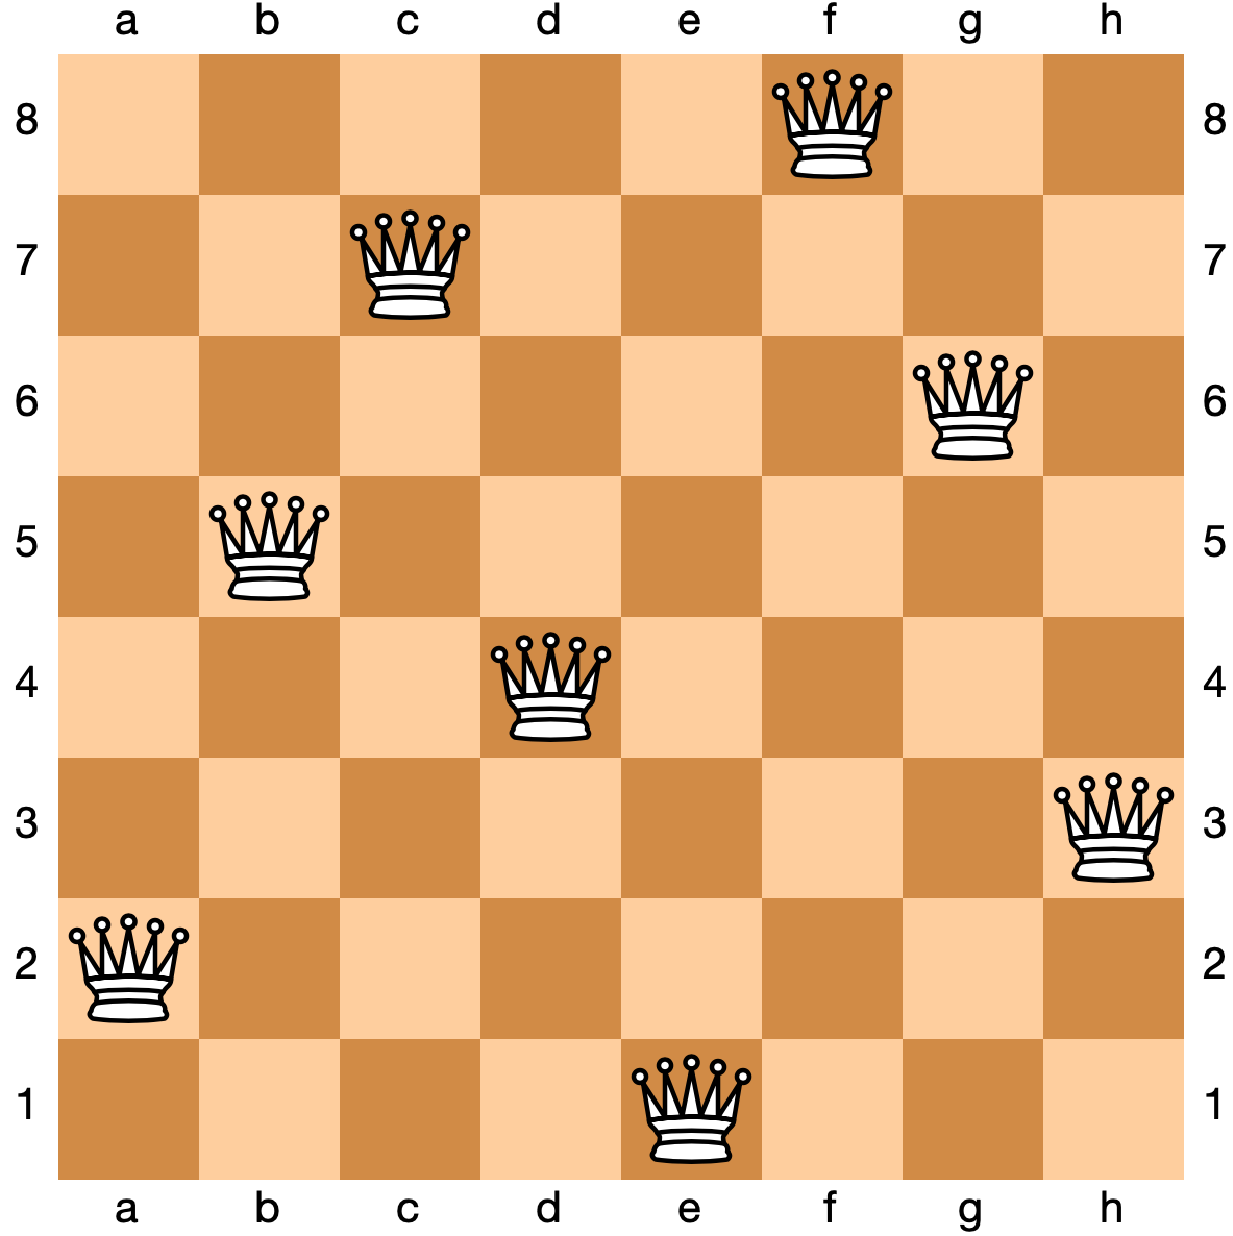
\epsfig{file=Figures/8-queens.pdf, scale=0.5}} 
  \caption{A solution of the 8-queens-problem.}
  \label{fig:8-queens.pdf}
\end{figure}
\FloatBarrier


\exerciseEng
The following exercise is taken from the book 
\href{https://www.amazon.de/Logeleien-Zweistein-ihren-Antworten-Wegner/dp/B006YF0VUE}{99 Logeleien von Zweistein}.
This book has been published 1968.  It is written by 
\href{http://de.wikipedia.org/wiki/Thomas_von_Randow}{Thomas von Randow}.

\begin{minipage}{0.95\linewidth}
  {\sl
    The gentlemen \emph{Amann}, \emph{Bemann}, \emph{Cemann} and \emph{Demann} are called --- not
    necessarily in the same order --- by their 
    first names \emph{Erich}, \emph{Fritz}, \emph{Gustav} and \emph{Heiner}. They are all married to
    exactly one woman. We also know the following about them and their wives: 
    \begin{enumerate}
    \item Either \emph{Amann's} first name is \emph{Heiner}, or \emph{Bemann's} wife is \emph{Inge}.
    \item If \emph{Cemann} is married to \emph{Josefa}, then --- \textbf{and only in this case} ---
          \emph{Klara's} husband is \textbf{not} called \emph{Fritz}.
    \item If \emph{Josefa's} husband is \textbf{not} called \emph{Erich}, then \emph{Inge} is married to
          \emph{Fritz}. 
    \item If \emph{Luise's} husband is called \emph{Fritz}, then \emph{Klara's} husband's first name is
          \textbf{not} \emph{Gustav}. 
    \item If the wife of \emph{Fritz} is called \emph{Inge}, then \emph{Erich} is \textbf{not} married to
          \emph{Josefa}. 
    \item If \emph{Fritz} is \textbf{not} married to \emph{Luise}, then \emph{Gustav's} wife's name is \emph{Klara}.
    \item Either \emph{Demann} is married to \emph{Luise}, or \emph{Cemann} is called \emph{Gustav}.
    \end{enumerate}
    What are the full names of these gentlemen, and what are their wives' first names?}
\end{minipage}
\vspace*{0.3cm}

\noindent
\textbf{Hint}: You should use the following propositional variables to solve the problem.
\begin{enumerate}
\item $\texttt{MaleName<}x\texttt{,}z\texttt{>}$ for any male first name $x$ and any surname $z$ expresses
  that the gentleman with first name $x$ has surname $z$.
\item $\texttt{Married<}x\texttt{,}y\texttt{>}$ for any male first name $x$ and any female first name $y$ expresses
  that the gentleman with first name $x$ is married to the lady with first name $y$.
\item $\texttt{FemaleName<}y\texttt{,}z\texttt{>}$ for any female first name $y$ and any last name $z$ expresses
  that the lady with first name $y$ has surname $z$. \eox
\end{enumerate}
I have provided the framework of a notebook at the following address:
\\[0.2cm]
\hspace*{1.3cm}
\href{https://github.com/karlstroetmann/Logic/blob/master/TypeScript/Chapter-4/Zweistein-Frame.ipynb}{\texttt{Chapter-4/Zweistein-Frame.ipynb}}
\\[0.2cm]
You should edit this notebook in order to solve the given problem. \eox



\subsection{The \href{https://en.wikipedia.org/wiki/Zebra_Puzzle}{Zebra Puzzle} \label{section:zebra}} 
The following logical puzzle appeared in the magazine
\href{https://en.wikipedia.org/wiki/Life_(magazine)}{Life International} 
on  December, $17^\textrm{th}$  in the year 1962:
\begin{itemize}
\item There are five houses.
\item The Englishman lives in the red house.
\item The Spaniard owns the dog.
\item Coffee is drunk in the green house.
\item The Ukrainian drinks tea.
\item The green house is immediately to the right of the ivory house.
\item The Old Gold smoker owns snails.
\item Kools are smoked in the yellow house.
\item Milk is drunk in the middle house.
\item The Norwegian lives in the first house.
\item The man who smokes Chesterfields lives in the house next to the man with the fox.
\item Kools are smoked in the house next to the house where the horse is kept.
\item The Lucky Strike smoker drinks orange juice.
\item The Japanese smokes Parliaments.
\item The Norwegian lives next to the blue house.
\end{itemize}
Furthermore, each of the five houses is painted in a different colour, their
inhabitants are of different nationalities, own different pets, drink different
beverages, and smoke different brands of cigarettes.  

Our task is to answers the following questions:
\begin{enumerate}
\item Who drinks water?
\item Who owns the zebra?
\end{enumerate}

In order to formulate this puzzle as a propositional formula we first have to
choose the appropriate propositional variables.  In order to express the fact
that the Englishman lives in the $i^\textrm{th}$ house we can use the variables
\\[0.2cm]
\hspace*{1.3cm}
$\texttt{English}\langle i \rangle$ \quad for $i=1,\cdots,5$.
\\[0.2cm]
The idea is that the variable $\texttt{English}\langle i \rangle$ is \texttt{true} iff the
Englishman lives in the  $i^\textrm{th}$ house.  In a similar way we use the
variables
\\[0.2cm]
\hspace*{1.3cm}
$\texttt{Spanish}\langle i \rangle$,\;
$\texttt{Ukrainian}\langle i \rangle$,\;
$\texttt{Norwegian}\langle i \rangle$,\; and 
$\texttt{Japanese}\langle i \rangle$
\\[0.2cm]
to encode where the people of different nationalities live.
The different drinks are encoded by the variables
\\[0.2cm]
\hspace*{1.3cm}
$\texttt{Coffee}\langle i \rangle$,\; $\texttt{Milk}\langle i \rangle$,\; $\texttt{OrangeJuice}\langle i \rangle$,\; $\texttt{Tea}\langle i \rangle$,\; and $\texttt{Water}\langle i \rangle$.
\\[0.2cm] 
The colours are encoded using the variables 
\\[0.2cm]
\hspace*{1.3cm}
$\texttt{Red}\langle i \rangle$,\;
$\texttt{Green}\langle i \rangle$,\;
$\texttt{Ivory}\langle i \rangle$,\;
$\texttt{Yellow}\langle i \rangle$,\; and $\texttt{Blue}\langle i \rangle$.
\\[0.2cm]
The pets are encoded using the variables
\\[0.2cm]
\hspace*{1.3cm}
$\texttt{Dog}\langle i \rangle$,\;
$\texttt{Snails}\langle i \rangle$,\;
$\texttt{Fox}\langle i \rangle$,\;
$\texttt{Horse}\langle i \rangle$,\;
and $\texttt{Zebra}\langle i \rangle$.
\\[0.2cm]
The cigarette brands are encoded as
\\[0.2cm]
\hspace*{1.3cm}
$\texttt{OldGold}\langle i \rangle$,\; $\texttt{Kools}\langle i \rangle$,\;
$\texttt{Chesterfields}\langle i \rangle$,\; $\texttt{Luckies}\langle i \rangle$,\; and
$\texttt{Parliaments}\langle i \rangle$.
\\[0.2cm]
We are using the angular brackets "$\langle$" and "$\rangle$" as part of the
variable names because our parser for propositional logic accepts these symbols
as part of variable names.  The parser would be confused if we would use the
normal parenthesis.  

\begin{figure}[!ht]
\centering
\begin{minted}[ frame         = lines, 
                 framesep      = 0.3cm, 
                 firstnumber   = 1,
                 bgcolor       = sepia,
                 numbers       = left,
                 numbersep     = -0.2cm,
                 xleftmargin   = 0.8cm,
                 xrightmargin  = 0.8cm,
                 ]{typescript}
    function varName(f: string, i: number): string {
        return `${f}<${i}>`;
    }
\end{minted}
\vspace*{-0.3cm}
\caption{The function $\texttt{varName}(f, i)$.}
\label{fig:var_f_i}
\end{figure}

In order to be able to write the conditions concisely, we introduce the function
$\texttt{varName}(f, i)$, which is shown in Figure \ref{fig:var_f_i}.  This function
takes a string $f$, where $f$ is a property like, e.g.~\texttt{Japanese} and an
integer $i \in \{1,\cdots,5\}$ and returns the string $f\langle i\rangle$.




\begin{figure}[!ht]
\centering
\begin{minted}[ frame         = lines, 
                 framesep      = 0.3cm, 
                 firstnumber   = 1,
                 bgcolor       = sepia,
                 numbers       = left,
                 numbersep     = -0.2cm,
                 xleftmargin   = 0.8cm,
                 xrightmargin  = 0.8cm,
               ]{typescript}
    function somewhere(x: string): Set<Literal> {
        return range(1, 5).map(i => varName(x, i))
    }
\end{minted}
\vspace*{-0.3cm}
\caption{The function \texttt{somewhere}.}
\label{fig:somewhere}
\end{figure}
The function $\texttt{somewhere}(x)$ that is shown in Figure \ref{fig:somewhere}
takes a string $x$ as its argument, where $x$ denotes a property like,
e.g.~\texttt{Japanese}.  It returns a clause that specifies that $x$ has to be
located in one of the five houses.  For example,  the call
$\texttt{somewhere('Japanese')}$ returns the clause
\\[0.2cm]
\hspace*{1.3cm}
\texttt{\{'Japanese<1>', 'Japanese<2>', 'Japanese<3>', 'Japanese<4>', 'Japanese<5>'\}}
\\[0.2cm]
as a \texttt{frozenset}.

\begin{figure}[!ht]
\centering
\begin{minted}[ frame         = lines, 
                 framesep      = 0.3cm, 
                 firstnumber   = 1,
                 bgcolor       = sepia,
                 numbers       = left,
                 numbersep     = -0.2cm,
                 xleftmargin   = 0.8cm,
                 xrightmargin  = 0.8cm,
               ]{typescript}
    function atMostOneAt(S: Set<string>, i: number): Set<Clause> {
        return atMostOne(S.map(x => varName(x, i)));
    }
\end{minted}
\vspace*{-0.3cm}
\caption{The function \texttt{atMostOneAt}(S, i)}
\label{fig:atMostOneAt}
\end{figure}

Given an set of properties $S$ and a house number $i$, the function
$\texttt{atMostOne}(S, i)$ returns a set of clauses that specifies that the
person living in house number $i$ has at most one of the properties from the set
$S$.  For example, if  
\\[0.2cm]
\hspace*{1.3cm}
$S = \{\texttt{"Japanese"}, \texttt{"Englishman"}, \texttt{"Spaniard"}, \texttt{"Norwegian"}, \texttt{"Ukranian"}\}$, 
\\[0.2cm]
then $\texttt{atMostOne}(S, 3)$ specifies that the inhabitant of house number 3
has at most one of the nationalities from the set $S$.   The implementation
makes use of the function \texttt{atMostOne} that is shown in Figure
\ref{fig:atMostOne} on page \pageref{fig:atMostOne}.

\begin{figure}[!ht]
\centering
\begin{minted}[ frame         = lines, 
                 framesep      = 0.3cm, 
                 firstnumber   = 1,
                 bgcolor       = sepia,
                 numbers       = left,
                 numbersep     = -0.2cm,
                 xleftmargin   = 0.8cm,
                 xrightmargin  = 0.8cm,
                 ]{typescript}
    function onePerHouse(S: Set<Variable>): Set<Clause> {
        const Result = S.map(x => somewhere(x));
        return Result.flatMap(range(1, 5), i => atMostOneAt(S, i));
    }
\end{minted}
\vspace*{-0.3cm}
\caption{The function \texttt{onePerHouse}.}
\label{fig:onePerHouse}
\end{figure}

The function $\texttt{onePerHouse}(S)$ takes a set $S$ of properties.  For
example, $S$ could be the set of the five nationalities.
In this case, the function would create a set of clauses that expresses that
there has to be a house where the Japanese lives, a house where the Englishman
lives, a house where the Spaniard lives, a house where the Norwegian lives, and
a house where the Ukranian lives.  Furthermore, the set of clauses would contain
clauses that express the fact that these five persons live in different houses.


\begin{figure}[!ht]
\centering
\begin{minted}[ frame         = lines, 
                 framesep      = 0.3cm, 
                 firstnumber   = 1,
                 bgcolor       = sepia,
                 numbers       = left,
                 numbersep     = -0.2cm,
                 xleftmargin   = 0.3cm,
                 xrightmargin  = 0.3cm,
               ]{typescript}
    function sameHouse(a: Variable, b: Variable): Set<Clause> {
        return flatMap(range(1, 5),
                       i => parseKNF(`${varName(a, i)} ↔ ${varName(b, i)}`));
    }
\end{minted}
\vspace*{-0.3cm}
\caption{The function $\texttt{sameHouse}(a, b)$.}
\label{fig:sameHouse}
\end{figure}

Given two properties $a$ and $b$ the function $\texttt{sameHouse}(a, b)$ that is
shown in Figure \ref{fig:sameHouse} computes
a set of clauses that specifies that if the inhabitant of house number $i$ has
the property $a$, then he also has the the property $b$ and vice versa.  For
example, $\texttt{sameHouse}(\texttt{"Japanese"}, \texttt{"Dog"})$ specifies
that the Japanese guy keeps a dog.  The function \texttt{parseKNF} that is used here takes a string, converts
it into a formula from propositional logic, and finally converts this formula into \textsc{Cnf}.

\begin{figure}[!ht]
\centering
\begin{minted}[ frame         = lines, 
                framesep      = 0.2cm, 
                firstnumber   = 1,
                bgcolor       = sepia,
                numbers       = left,
                numbersep     = 0.3cm,
                xleftmargin   = 0.0cm,
                xrightmargin  = 0.0cm,
              ]{typescript}
function nextTo(a: Variable, b: Variable): Set<Clause> {
    const Formulas = [
        `${varName(a, 1)} → ${varName(b, 2)}`, // House 1
        ...[2, 3, 4].map(
          i => `${varName(a, i)} → ${varName(b, i-1)} ∨ ${varName(b, i+1)}`), 
        `${varName(a, 5)} → ${varName(b, 4)}`  // House 5
    ];
    const Result = set<Clause>();
    return Result.flatMap(Formulas, formula => parseKNF(formula));
}
\end{minted}
\vspace*{-0.3cm}
\caption{nextTo} %$
\label{fig:nextTo}
\end{figure}
Given to properties $a$ and $b$ the function $\texttt{nextTo}(a, b)$ computes a
set of clauses that specifies that the inhabitants with properties $a$ and $b$
are direct neighbours.  For example, $\texttt{nextTo}(\texttt{'Japanese'}, \texttt{'Dog'})$
specifies that the Japanese guy lives next to the guy who keeps a dog. 
This is specified as follows:
\begin{enumerate}
\item If the person with property $a$ lives in the first house, then the person with property $b$ has to live
      in the second house.
\item If the person with property $a$ lives in one of the houses $i$ where $i \in \{ 2, 3, 4 \}$, then
      the person with property $b$ either lives to the left in house $i-1$ or to the right in house $i+1$.
\item If the person with property $a$ lives in the fifth house, then the person with property $b$ has to live
      in the fourth house.
\end{enumerate}

\begin{figure}[!ht]
\centering
\begin{minted}[ frame         = lines, 
                 framesep      = 0.3cm, 
                 firstnumber   = 1,
                 bgcolor       = sepia,
                 numbers       = left,
                 numbersep     = -0.2cm,
                 xleftmargin   = 0.0cm,
                 xrightmargin  = 0.0cm,
               ]{typescript}
    function leftTo(a: Variable, b: Variable): Set<Clause> {
        const Formulas = [
            ...[1, 2, 3, 4].map(i => `${varName(a, i)} → ${varName(b, i + 1)}`),
            `¬${varName(a, 5)}`
        ];
        const Result = set<Clause>();
        return Result.flatMap(Formulas, formula => parseKNF(formula));
    }
\end{minted}
\vspace*{-0.3cm}
\caption{The function \texttt{leftTo}.} %$
\label{fig:leftTo}
\end{figure}

Given to properties $a$ and $b$ the function $\texttt{leftTo}(a, b)$ computes a
list of clauses that specifies that the inhabitants with properties $a$ lives in
the house to the left of the inhabitant who has property $b$.  For example,
$\texttt{livesTo}(\texttt{'Japanese'}, \texttt{'Dog'})$ specifies that the
Japanese guy lives in the house to the left of the house where there is a dog.

\begin{figure}[!ht]
\centering
\begin{minted}[ frame         = lines, 
                 framesep      = 0.3cm, 
                 firstnumber   = 1,
                 bgcolor       = sepia,
                 numbers       = left,
                 numbersep     = 0.3cm,
                 xleftmargin   = -0.1cm,
                 xrightmargin  = -0.1cm,
               ]{typescript}
const Nations = set("English", "Spanish", "Ukrainian", "Norwegian", "Japanese");
const Drinks  = set("Coffee", "Tea", "Milk", "OrangeJuice", "Water");
const Pets    = set("Dog", "Snails", "Horse", "Fox", "Zebra");
const Brands  = set("Luckies", "Parliaments", "Kools", "Chesterfields", "OldGold");
const Colours = set("Red", "Green", "Ivory", "Yellow", "Blue");
\end{minted}
\vspace*{-0.3cm}
\caption{Definition of the properties.}
\label{fig:properties}
\end{figure}

In order to be able to formulate the different conditions conveniently, we define the sets
shown in Figure \ref{fig:properties}.

\begin{figure}[!ht]
\centering
\begin{minted}[ frame         = lines, 
                 framesep      = 0.3cm, 
                 firstnumber   = 1,
                 bgcolor       = sepia,
                 numbers       = left,
                 numbersep     = 0.2cm,
                 xleftmargin   = 0.0cm,
                 xrightmargin  = 0.0cm,
               ]{typescript}
function allClauses(): Set<Clause> {
    const Result = set<Clause>();
    // Every property category gets exactly one house
    Result.flatMap([Nations, Drinks, Pets, Brands, Colours], S => onePerHouse(S));
    const puzzleClues = [
        // The Englishman lives in the red house.
        sameHouse("English", "Red"),
        // The Spaniard owns the dog.
        sameHouse("Spanish", "Dog"), 
        // Coffee is drunk in the green house.
        sameHouse("Coffee", "Green"),
        // The Ukrainian drinks tea.
        sameHouse("Ukrainian", "Tea"),
        // The green house is immediately to the right of the ivory house.
        leftTo("Ivory", "Green"), 
        // The Old Gold smoker owns snails.
        sameHouse("OldGold", "Snails"), 
        // Kools are smoked in the yellow house.
        sameHouse("Kools", "Yellow"), 
        // Milk is drunk in the middle house.
        parseKNF(varName("Milk", 3)), 
        // The Norwegian lives in the first house.
        parseKNF(varName("Norwegian", 1)), 
        // Chesterfields smoker lives next to the fox owner.
        nextTo("Chesterfields", "Fox"),                                         
        // Kools are smoked next to the horse.
        nextTo("Kools", "Horse"), 
        // The Lucky Strike smoker drinks orange juice.
        sameHouse("Luckies", "OrangeJuice"),                                              
        // The Japanese smokes Parliaments.
        sameHouse("Japanese", "Parliaments"), 
        // The Norwegian lives next to the blue house.
        nextTo("Norwegian", "Blue") 
    ];
    return Result.flatMap(puzzleClues, S => S);
}
\end{minted}
\vspace*{-0.3cm}
\caption{The function \texttt{allClauses}.}
\label{fig:allClauses}
\end{figure}
The function \texttt{allClauses} in Figure \ref{fig:allClauses} computes a set of clauses that encodes the
conditions of the zebra puzzle.  If we solve these clauses with the algorithm of
Davis and Putnam, we get the solution that is shown in Figure \ref{fig:zebra}.

\begin{figure}[!ht]
  \centering
  \framebox{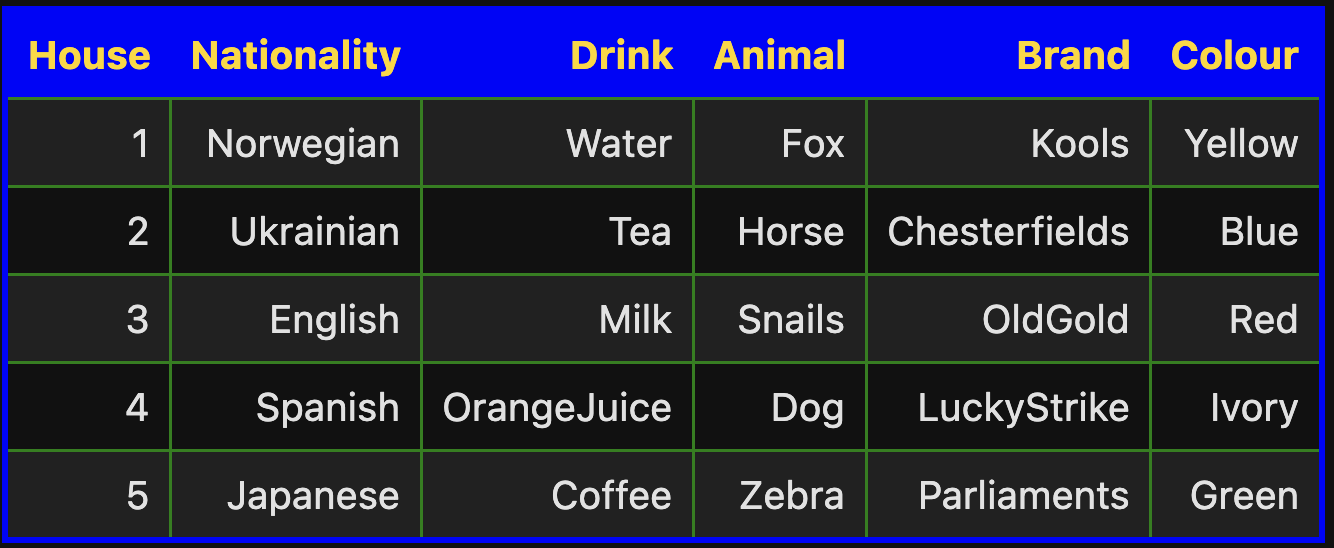
\epsfig{file=Figures/zebra.png, scale=0.7}} 
  \caption{The solution of the zebra puzzle.}
  \label{fig:zebra}
\end{figure}

\pagebreak
\vspace*{\fill}

\pagebreak

\exerciseEng
\textbf{\large The Trial of the Nine Portals} \\
In an era of high-stakes romantic gambles and questionable parenting, there reigned a King—a man whose passion
for discrete mathematics far outweighed his concern for his daughter’s emotional well-being.  

Determined that his heir-in-law be a man of cold, calculating intellect rather than mere royal vibes, the
King broadcast a decree across the realm. It was essentially a LinkedIn job posting for a Prince, but with
significantly higher mortality rates. 

Eventually, a Prince arrived. The King led him to a corridor containing \textbf{nine identical doors}, behind
which lay one of three fates: 
\begin{enumerate}
\item \textbf{The Princess}:     The ultimate prize (and a lifetime of complex family dinners).
\item \textbf{A Ravenous Tiger}: An immediate career change to \href{https://www.whiskas.de/}{cat food}.
\item \textbf{Void \& Dust}:     Empty rooms for those who enjoy the solace of disappointment.
\end{enumerate}

\noindent
\textbf{\large The Royal Logic Protocol} \\
The King, smirking with the malice of a tenured professor, pointed to the cryptic signs etched into each
door. ``To ensure you aren't a total dullard," he barked, ``you must navigate this gauntlet using the
\textbf{Infallible Laws of Logic}:'' 
\begin{enumerate}
\item \textbf{The Path of Teeth}: If a room contains a \blue{Tiger}, the inscription on that door is a
      \blue{bold-faced lie}, as blatantly false as the answer you get when you asked a tenured professor the stupid
      question ``Was kommt in der Klausur?''.
\item \textbf{The Path of Matrimony:} If the room contains the \blue{Princess}, the inscription is
      \blue{absolute truth}.
\item \textbf{The Path of the Void}: If the room is empty, we enter the realm of bureaucratic inconsistency.
      Either \textbf{all} signs on empty rooms are true, or \textbf{all} of them are false. There is no middle
      ground, only total logical uniformity or total deception. 
\end{enumerate}
``Choose \href{https://www.youtube.com/watch?v=c3RN9zz77Cs}{wisely},'' the King added, adjusting his crown.
``For in this kingdom, love isn't just a battlefield—it's a multi-choice logic exam where the penalty for a 'C'
is being digested.''  

The Prince looked at the doors. The doors looked back. Somewhere, a tiger sharpened its claws, and the Princess
wondered if she should have just joined a convent.

The prince then read the inscriptions. These were as follows:
\begin{enumerate}
\item Room: The princess is in a room with an odd number and
      there is no tiger in the rooms with an even number.
\item Room: This room is empty.
\item Room: The inscription on Room No. 5 is \texttt{true}, the inscription on Room No. 7 is \texttt{false},
      and there is a tiger in Room No. 3.
\item Room: The inscription on Room No. 1 is \texttt{false}, there is no tiger in Room No. 8,
      and the inscription on Room No. 9 is \texttt{true}.
\item Room: If the inscription on Room No. 2 or on Room No. 4 is \texttt{true},
      then there is no tiger in Room No. 1.
\item Room: The inscription on Room No. 3 is \texttt{false}, the princess is in Room No. 2,
      and there is no tiger in Room No. 2.
\item Room: The princess is in Room No. 1 and the inscription on Room No. 5 is \texttt{true}.
\item Room: There is no tiger in this room and Room No. 9 is empty.
\item Room: Neither in this room nor in Room No. 1 is there a tiger, and moreover, the
      inscription on Room No. 6 is \texttt{true}.
\end{enumerate} 
I have provided the framework of a notebook at the following address:
\\[0.2cm]
\hspace*{1.3cm}
\href{https://github.com/karlstroetmann/Logic/blob/master/TypeScript/Chapter-4/Prince-Tiger-Frame.ipynb}{\texttt{Chapter-4/Prince-Tiger-Frame.ipynb}}
\\[0.2cm]
You should edit this notebook in order to solve the given problem. \eox
\vspace*{1cm}


\section{Sudoku and PicoSat}
As a final example we will solve a \href{https://en.wikipedia.org/wiki/Sudoku}{Sudoku} puzzle.  In particular,
we will solve an instance of a Sudoku puzzle that was created by Arto Inkala.  He claims that this is the
\href{https://abcnews.go.com/blogs/headlines/2012/06/can-you-solve-the-hardest-ever-sudoku}{hardest solvable instance}
of a Sudoku puzzle.  Figure \ref{fig:sudoku.png} shows the Sudoku created by Arto Inkala.

\begin{figure}[!ht]
  \centering
  \framebox{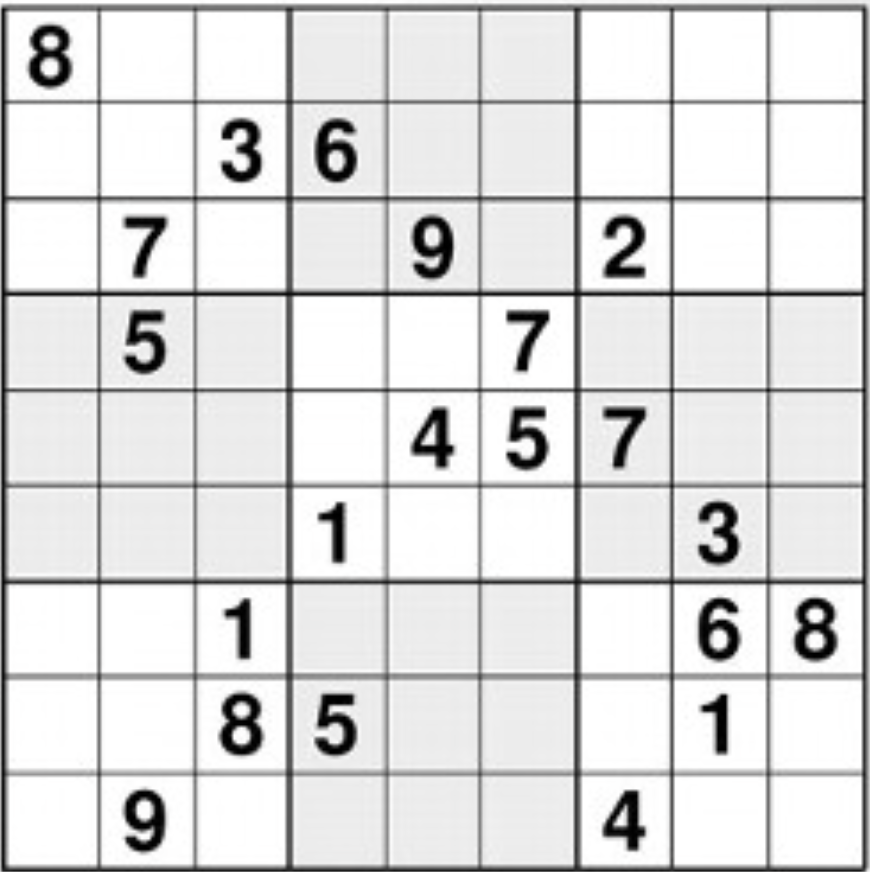
\epsfig{file=Figures/sudoku.png, scale=0.5}} 
  \caption{The Sudoku puzzle created by Arto Inkala.}
  \label{fig:sudoku.png}
\end{figure}

A Sudoku puzzle is a logic-based, combinatorial number-placement puzzle. The objective is to fill a
$9 \times 9$ grid with digits from the set $\{1, \cdots, 9\}$ so that each column, each row, and each of the
nine $3 \times 3$ subgrids that compose the grid (also called "boxes") contain all of these digits exactly
once.  The puzzle is given as a partially completed grid.  A well-posed puzzle must have a single unique
solution.

In order to formulate a Sudoku as a satisfiablity problem from propositional logic, we will use the following
set of propositional variables:
\\[0.2cm]
\hspace*{1.3cm}
$\mathcal{P} = \bigl\{ Q_{r,c,d} \mid r \in \{1,\cdots, 9\} \wedge c \in \{1,\cdots, 9\} \wedge r \in \{1,\cdots, 9\} \bigl\}$
\\[0.2cm]
For a given digit $d \in \{1, \cdots, 9\}$, a given row $r \in \{1, \cdots, 9\}$, and a given column
$c \in \in \{1, \cdots, 9\}$, the variable $Q_{r,c,d}$ is supposed to be \texttt{true} if $d$ is the digit in
row $r$ and column $c$ of the Sudoku.  Note that this means that we have $9^3 = 729$ different propositional
variables.  In our implementation we will use the function \texttt{varName} shown in
Figure \ref{fig:sudoku-var} to create these variables.

\begin{figure}[!ht]
\centering
\begin{minted}[ frame         = lines, 
                 framesep      = 0.3cm, 
                 firstnumber   = 1,
                 bgcolor       = sepia,
                 numbers       = left,
                 numbersep     = -0.2cm,
                 xleftmargin   = 0.8cm,
                 xrightmargin  = 0.8cm,
               ]{typescript}
    function varName(row: number, col: number, digit: number): string {
        return `Q<${row},${col},${digit}>`;
    }
\end{minted}
\vspace*{-0.3cm}
\caption{The function \texttt{varName}.}
\label{fig:sudoku-var}
\end{figure} %$

The Sudoku itself is created by the function \texttt{create\_puzzle} shown in Figure
\ref{fig:sudoku-create-puzzle} on page \pageref{fig:sudoku-create-puzzle}.  In this function, the puzzle is
represented as a list of lists.  Each of these lists represents a row.  The inner lists contain digits and the
character \texttt{"*"}.  This character represent those digits that are initially unknown and whose value have
to be computed.

\begin{figure}[!ht]
\centering
\begin{minted}[ frame         = lines, 
                 framesep      = 0.3cm, 
                 firstnumber   = 1,
                 bgcolor       = sepia,
                 numbers       = left,
                 numbersep     = -0.2cm,
                 xleftmargin   = 0.8cm,
                 xrightmargin  = 0.8cm,
               ]{typescript}
function createPuzzle(): (number | '*')[][] {
    return [[ 8 , '*', '*', '*', '*', '*', '*', '*', '*'],
            ['*', '*',  3,   6 , '*', '*', '*', '*', '*'],
            ['*',  7 , '*', '*',  9 , '*',  2 , '*', '*'],
            ['*',  5 , '*', '*', '*',  7 , '*', '*', '*'],
            ['*', '*', '*', '*',  4 ,  5 ,  7 , '*', '*'],
            ['*', '*', '*',  1 , '*', '*', '*',  3 , '*'],
            ['*', '*',  1 , '*', '*', '*', '*',  6 ,  8 ],
            ['*', '*',  8 ,  5 , '*', '*', '*',  1 , '*'],
            ['*',  9 , '*', '*', '*', '*',  4 , '*', '*']
    ];
}
\end{minted}
\vspace*{-0.3cm}
\caption{The function \texttt{create\_puzzle}.}
\label{fig:sudoku-create-puzzle}
\end{figure}

In our implementation we will use functions \texttt{atMostOne} that we have already seen in Figure
\ref{fig:atMostOne} on page \pageref{fig:atMostOne} that expresses that at most one of a given set of
propositional variables is \texttt{true}.  Furthermore, we will use the auxiliary function
$\texttt{atLeastOne}(V)$ which takes a set of propositional variables $V$ and which returns a formula in
conjunctive normal form in set notation that is \texttt{true} if and only if at least one of the variables in
$V$ is \texttt{true}.  Note that in set notation we have
\\[0.2cm]
\hspace*{1.3cm}
$\texttt{atLeastOne}(V) = \bigl\{ V \bigr\}$.
\\[0.2cm]
The reason is that in set notation  $V$ is interpreted as a clause, i.e.~as a disjunction of its variables.
Using these two functions we can then define a function $\texttt{exactlyOne}(V)$ that
takes a set of variables and returns \texttt{true} iff exactly one of the variables in $V$ is \texttt{true}.
The implementation is shown in Figure \ref{fig:sudoku-exactly}.

\begin{figure}[!ht]
\centering
\begin{minted}[ frame         = lines, 
                 framesep      = 0.3cm, 
                 firstnumber   = 1,
                 bgcolor       = sepia,
                 numbers       = left,
                 numbersep     = -0.2cm,
                 xleftmargin   = 0.8cm,
                 xrightmargin  = 0.8cm,
                 ]{typescript}
    function atLeastOne(S: Set<Variable>): Set<Clause> {
        return set(S);
    }
    function exactlyOne(S: Set<Variable>): Set<Clause> {
        return atMostOne(S).union(atLeastOne(S));
    }
\end{minted}
\vspace*{-0.3cm}
\caption{The functions \texttt{atLeastOne} and \texttt{exactlyOne}.}
\label{fig:sudoku-exactly}
\end{figure}



\begin{figure}[!ht]
\centering
\begin{minted}[ frame         = lines, 
                 framesep      = 0.3cm, 
                 firstnumber   = 1,
                 bgcolor       = sepia,
                 numbers       = left,
                 numbersep     = -0.2cm,
                 xleftmargin   = 0.3cm,
                 xrightmargin  = 0.3cm,
               ]{typescript}
    type Position = Tuple<[number, number]>;
               
    function exactlyOneForDigit(L: Set<Position>, digit: number): Set<Clause> {
        return exactlyOne(L.map(([row, col]) => varName(row, col, digit)));
    }
\end{minted}
\vspace*{-0.3cm}
\caption{The function \texttt{exactlyOneForDigit}.}
\label{fig:sudoku-exactlyOneForDigit}
\end{figure}

Figure \ref{fig:sudoku-exactlyOneForDigit} show the implementation of the function
$\texttt{exactlyOneForDigit}(L, d)$.

First, we define the type \texttt{Position}, which is a pair of the form $(r, c)$, where $r \in \{1,\cdots,9\}$
specifies the row, while $c \in \{1,\cdots,9\}$ specifies the column of the position.

The function $\texttt{exactlyOneForDigit}(L, d)$ takes a set $L$ of Positions and a digit $d$ as its arguments.
The function $\texttt{exactlyOnce}$ computes a set of formulas $L$ that express that the digit $d$ 
occurs in exactly one of the positions in $L$.



\begin{figure}[!ht]
\centering
\begin{minted}[ frame         = lines, 
                 framesep      = 0.3cm, 
                 firstnumber   = 1,
                 bgcolor       = sepia,
                 numbers       = left,
                 numbersep     = -0.2cm,
                 xleftmargin   = 0.8cm,
                 xrightmargin  = 0.8cm,
                 ]{typescript}
    function exactlyOneForEveryDigit(L: Set<Position>): Set<Clause> {
        return flatMap(range(1, 9), d => exactlyOneForDigit(L, d));
    }
\end{minted}
\vspace*{-0.3cm}
\caption{The function \texttt{exactlyOneForEveryDigit}.}
\label{fig:sudoku-exactlyOneDigit}
\end{figure}

The function $\texttt{exactlyOneForEveryDigit}(L)$ takes a set $L$ cell positions as its argument.  
It returns a set of formulas expressing that all of the nine digits occurs at exactly one position in the list `L`.

\begin{figure}[!ht]
\centering
\begin{minted}[ frame         = lines, 
                 framesep      = 0.3cm, 
                 firstnumber   = 1,
                 bgcolor       = sepia,
                 numbers       = left,
                 numbersep     = -0.2cm,
                 xleftmargin   = 0.8cm,
                 xrightmargin  = 0.8cm,
                 ]{typescript}
    function exactlyOneDigit(row: number, col: number): Set<Clause> {
        return exactlyOne(range(1, 9).map(d => varName(row, col, d)));
    }
\end{minted}
\vspace*{-0.3cm}
\caption{The function \texttt{exactlyOneDigit}.}
\label{fig:sudoku-exactlyOneDigit}
\end{figure}

The function $\mathtt{exactlyOneDigit}(r, c)$ takes a row $r$ and a column $c$ as its arguments.
It returns a set of clauses expressing that there is exactly one digit in the given cell.

Furthermore, we need a function encoding the constraints form the puzzle itself.
This function is called \texttt{constraintsFromPuzzle} and its implementation is shown in Figure
\ref{fig:sudoku-constraintsFromPuzzle} on page \pageref{fig:sudoku-constraintsFromPuzzle}.
For example, the given puzzle demands that the digit in row 2 and column 4 is the digit $6$.
This can be expressed as the formula $Q_{2,3,6}$.  In set notation this formula takes the form
\\[0.2cm]
\hspace*{1.3cm}
$\bigl\{ \{Q_{2,3,6}\} \bigr\}$.
\\[0.2cm]
Of course, we have to take the union of all these formula.  This leads to the code shown in Figure
\ref{fig:sudoku-constraintsFromPuzzle} on page \pageref{fig:sudoku-constraintsFromPuzzle}.
Note that we have to provide \texttt{row+1} and \texttt{col+1} as arguments to the function \texttt{varName} since
in TypeScript list indices start with $0$.

\begin{figure}[!ht]
\centering
\begin{minted}[ frame         = lines, 
                 framesep      = 0.3cm, 
                 firstnumber   = 1,
                 bgcolor       = sepia,
                 numbers       = left,
                 numbersep     = -0.2cm,
                 xleftmargin   = 0.0cm,
                 xrightmargin  = 0.0cm,
                 ]{typescript}
    function constraintsFromPuzzle(): Set<Clause> {
        const Puzzle  = createPuzzle();
        const Indices = range(1, 9);    
        return Indices.cartesianProduct(Indices).filterMap(
            ([r, c]) => Puzzle[r-1][c-1] != '*',
            ([r, c]) => set(varName(r, c, Puzzle[r-1][c-1] as number)));
    }
\end{minted}
\vspace*{-0.3cm}
\caption{The function \texttt{constraintsFromPuzzle}}
\label{fig:sudoku-constraintsFromPuzzle}
\end{figure}

Finally, we have to combine all constraints of the puzzle.  This is done with the function \\
\texttt{allConstraints} shown in Figure \ref{fig:sudoku-allConstraints} shown on page \pageref{fig:sudoku-allConstraints}.

\begin{figure}[!ht]
\centering
\begin{minted}[ frame         = lines, 
                 framesep      = 0.3cm, 
                 firstnumber   = 1,
                 bgcolor       = sepia,
                 numbers       = left,
                 numbersep     = -0.2cm,
                 xleftmargin   = 0.0cm,
                 xrightmargin  = 0.0cm,
               ]{typescript}
    function getBlockCells(r: number, c: number): Set<Tuple<[number, number]>> {
        return range(1, 3).cartesianProduct(range(1, 3)).map(
            ([row, col]) => tpl(r * 3 + row, c * 3 + col)
        );
    }
    function allConstraints(): Set<Clause> {
        // 1. Start with constraints from the puzzle
        const Clauses = constraintsFromPuzzle();
        // 2. There is exactly one digit in every field
        Clauses.flatMap(
            range(1, 9).cartesianProduct(range(1, 9)), 
            ([row, col]) => exactlyOneDigit(row, col)
        );
        // 3. All entries in a row are unique
        Clauses.flatMap(
            range(1, 9), 
            row => exactlyOneForEveryDigit(range(1, 9).map(col => tpl(row, col)))
        );
        // 4. All entries in a column are unique
        Clauses.flatMap(
            range(1, 9), 
            col => exactlyOneForEveryDigit(range(1, 9).map(row => tpl(row, col)))
        );
        // 5. All entries in a 3 times 3 square are unique
        const block = range(0, 2).cartesianProduct(range(0, 2));
        Clauses.flatMap(block,
                        ([r, c]) => exactlyOneForEveryDigit(getBlockCells(r, c)));
        return Clauses;
    }  
\end{minted}
\vspace*{-0.3cm}
\caption{The function \texttt{allConstraints}.}
\label{fig:sudoku-allConstraints}
\end{figure}
The Jupyter notebook showing the resulting program is available at:
\\[0.2cm]
\hspace*{1.3cm}
\href{https://github.com/karlstroetmann/Logic/blob/master/TypeScript/Chapter-4/10-Sudoku.ipynb}{\texttt{Chapter-4/10-Sudoku.ipynb}}

\FloatBarrier

\subsection{Logic Solver}
Unfortunately, solving the resulting set of clauses takes about 21 minutes.  Fortunately, there is a version
of the Davis-Putnam algorithm that is implemented in \texttt{JavaScript}.  This solver is called
\href{https://github.com/meteor/logic-solver}{Logic Solver} and is based on \href{http://minisat.se/}{MiniSat}.

In \textsl{MiniSat} formulas are represented as follows:
\begin{itemize}
    \item \textbf{Boolean variables} are implicitly declared by using strings (e.g., \texttt{"p"}, \texttt{"q"}, \texttt{"r"}).
    \item \textbf{Negations} are represented by a preceding minus sign in the string (e.g., \texttt{"-q"} for $\neg q$). Alternatively, \texttt{Logic.not(...)} could be used.
    \item \textbf{Clauses} are constructed using \texttt{Logic.or(...)}, with strings serving as literals.
    \item The problem is built as a set of clauses (Conjunctive Normal Form, CNF) by adding each clause
      individually using \texttt{solver.require(...)}. This corresponds to a large conjunction of all clauses.
    \item The solver is initialized with \texttt{new Logic.Solver()}.
    \item The satisfiability check is performed using \texttt{solver.solve()}.
    \item If the formula is satisfiable, \texttt{solve()} returns a solution object, from which the array of
          true variables can be retrieved using \texttt{getTrueVars()}. Otherwise, \texttt{null} is returned. 
\end{itemize}
As an example, the formula 
$$ (\neg p \vee  q \vee \neg r) \wedge (p \vee \neg q \vee r) \wedge (p \vee q \vee \neg r) \wedge (p \vee q \vee r), $$
which is in conjunctive normal form, is represented by the following code:
\begin{verbatim}
    const solver = new Logic.Solver();
    solver.require(Logic.or("-p", "q", "-r"));
    solver.require(Logic.or("p", "-q", "r"));
    solver.require(Logic.or("p", "q", "-r"));
    solver.require(Logic.or("p", "q", "r"));
\end{verbatim}

\subsubsection{Transforming Clauses into PyCoSat Format}
In order to use \textsl{PicoSat} to solve the Sudoku discussed earlier, we need a function that transforms a
formula that is in conjunctive normal form into the format of \textsl{PicoSat}.  Furthermore, we need  a function that can translate a solution found by \textsl{PicoSat} back into our format.

The function \texttt{findVariables(Clauses)} in Figure \ref{fig:sudoku-findVariables} on page
\pageref{fig:sudoku-findVariables} takes a set of clauses and returns the set of all propositional variables
occurring in this set.


\begin{figure}[!ht]
\centering
\begin{minted}[ frame         = lines, 
                 framesep      = 0.3cm, 
                 firstnumber   = 1,
                 bgcolor       = sepia,
                 numbers       = left,
                 numbersep     = -0.2cm,
                 xleftmargin   = 0.8cm,
                 xrightmargin  = 0.8cm,
               ]{typescript}
    def findVariables(Clauses):
        Variables = set()
        for Clause in Clauses:
            for literal in Clause:
                match literal:
                    case ('¬', var): Variables |= { var }
                    case var       : Variables |= { var }
        return Variables
\end{minted}
\vspace*{-0.3cm}
\caption{The function \texttt{findVariables}.}
\label{fig:sudoku-findVariables}
\end{figure}

The function \texttt{numberVariables(Clauses)} takes a set of clauses as input.  It returns two dictionaries:
\begin{enumerate}
\item The dictionary \texttt{Var2Int} maps every propositional variable occurring in \texttt{Clauses} to a
      unique natural number. 
\item The dictionary \texttt{Int2Var} is the mapping that is inverse to the dictionary \texttt{Var2Int}.
      Hence it maps the natural numbers back to propositional variables.
\end{enumerate}

\begin{figure}[!ht]
\centering
\begin{minted}[ frame         = lines, 
                 framesep      = 0.3cm, 
                 firstnumber   = 1,
                 bgcolor       = sepia,
                 numbers       = left,
                 numbersep     = -0.2cm,
                 xleftmargin   = 0.8cm,
                 xrightmargin  = 0.8cm,
               ]{typescript}
    def numberVariables(Clauses):
        Variables = findVariables(Clauses)
        count     = 1
        Var2Int   = {}
        Int2Var   = {}
        for variable in Variables:
            Var2Int[variable] = count
            Int2Var[count   ] = variable
            count += 1
        return Var2Int, Int2Var             
\end{minted}
\vspace*{-0.3cm}
\caption{The function \texttt{numberVariables}}
\label{fig:sudoku-numberVariables}
\end{figure}

\pagebreak
Figure \ref{fig:sudoku-format} shows the remaining auxiliary functions that are necessary to transform a
formula represented as a set of clauses into the format of PicoSat.
\begin{enumerate}
\item The function \texttt{literal2int} takes a literal and transforms this literal into an integer
      representing the literal. If the literal is a negated variable, the integer is negative, else it is
      positive. \texttt{Var2Int} is a dictionary mapping propositional variables to natural numbers.
\item The function \texttt{clause2pyco(Clause, Var2Int)} transforms a set of literals into a list of integers.
      \texttt{Var2Int} is a dictionary mapping the propositional variables to natural numbers. 
\item The function \texttt{clauses2pyco(Clauses, Var2Int)} transforms a set of clauses into a list of lists of
      integers. \texttt{Var2Int} is a dictionary mapping the propositional variables to natural numbers.  
\item The function \texttt{int2var(Numbers, Int2Var)} takes a list of numbers representing a set of literals and returns
      the associated list of literals.  \texttt{Int2Var} is a dictionary mapping natural numbers to
      propositional variables.     
\end{enumerate}

\begin{figure}[!ht]
\centering
\begin{minted}[ frame         = lines, 
                 framesep      = 0.3cm, 
                 firstnumber   = 1,
                 bgcolor       = sepia,
                 numbers       = left,
                 numbersep     = -0.2cm,
                 xleftmargin   = 0.8cm,
                 xrightmargin  = 0.8cm,
               ]{typescript}
    def literal2int(literal, Var2Int):
        match literal:
            case ('¬', var): return -Var2Int[var]
            case var       : return  Var2Int[var]
    
    def clause2pyco(Clause, Var2Int):
        return [literal2int(literal, Var2Int) for literal in Clause]
    
    def clauses2pyco(Clauses, Var2Int):
        return [clause2pyco(clause, Var2Int) for clause in Clauses ]
    
    def int2var(Numbers, Int2Var):
        Result = set()
        for n in Numbers:
            if n > 0:
                Result |= {frozenset({Int2Var[n]})}
            else: 
                Result |= {frozenset({ ('¬', Int2Var[-n]) })}
        return Result
\end{minted}
\vspace*{-0.3cm}
\caption{Some axilliary functions to transform clauses into the format of PicoSat.}
\label{fig:sudoku-format}
\end{figure}

The Jupyter notebook showing the resulting program is available at:
\\[0.2cm]
\hspace*{0.3cm}
\href{https://github.com/karlstroetmann/Logic/blob/master/TypeScript/Chapter-4/11-PicoSat-Sudoku.ipynb}{\texttt{github.com/karlstroetmann/Logic/blob/master/TypeScript/Chapter-4/11-PicoSat-Sudoku.ipynb}}

\pagebreak


\section{Check Your Comprehension}
\begin{enumerate}[(a)]
\item How have we defined the set of propositional logic formulas?
\item How have we defined the semantics of propositional logic formulas?
\item How do we represent propositional logic formulas in \textsl{TypeScript}?
\item What is a tautology?
\item How can we transform propositional logic formula into conjunctive normal
      form?
\item Define the notion of an inference rule.
\item when is  an inference rule correct?
\item Define the cut rule.
\item How did we define the proof concept $M \vdash C$?
\item What is a saturated set of clauses?
\item What are the two most important properties of the proof concept $\vdash$?
\item Assume that $M$ is a saturated set of clauses. How can we define a propositional interpretation
      $\mathcal{I}$ such that $\mathcal{I}(C) = \mathtt{true}$ for all $C \in M$?
\item How did we define the notion of a set of clauses being solvable?
\item Do you know how the algorithm of Davis and Putnam works?
\item Can you code a logical puzzle as a propositional formula?
\end{enumerate}


%\input{compact-barwise}

%%% Local Variables: 
%%% mode: latex
%%% TeX-master: "logic"
%%% End: 
